\documentclass[journal]{IEEEtran}
\usepackage{cite}
\usepackage[pdftex]{graphicx}
\graphicspath{{./images/}}

% *** MATH PACKAGES ***
\usepackage[cmex10]{amsmath}
% *** SPECIALIZED LIST PACKAGES ***
\usepackage{algorithmic}
\usepackage{bookmark}
\usepackage{multirow}
% *** ALIGNMENT PACKAGES ***
\usepackage{array}
\usepackage{mdwmath}
\usepackage{mdwtab}
\usepackage{eqparbox}
% *** TIKZ ***
% Required packages and libraries
\usepackage {tikz}
\usetikzlibrary {patterns}
\usepackage{tkz-euclide}
% \usetkzobj{all}


% \usepackage{tikzpicture} %preamble

% *** SUBFIGURE PACKAGES ***
\usepackage[tight,footnotesize]{subfigure}
% subfigure.sty was written by Steven Douglas Cochran. This package makes it
% easy to put subfigures in your figures. e.g., "Figure 1a and 1b". For IEEE
% work, it is a good idea to load it with the tight package option to reduce
% the amount of white space around the subfigures. subfigure.sty is already
% installed on most LaTeX systems. The latest version and documentation can
% be obtained at:
% http://www.ctan.org/tex-archive/obsolete/macros/latex/contrib/subfigure/
% subfigure.sty has been superceeded by subfig.sty.



%\usepackage[caption=false]{caption}
%\usepackage[font=footnotesize]{subfig}
% subfig.sty, also written by Steven Douglas Cochran, is the modern
% replacement for subfigure.sty. However, subfig.sty requires and
% automatically loads Axel Sommerfeldt's caption.sty which will override
% IEEEtran.cls handling of captions and this will result in nonIEEE style
% figure/table captions. To prevent this problem, be sure and preload
% caption.sty with its "caption=false" package option. This is will preserve
% IEEEtran.cls handing of captions. Version 1.3 (2005/06/28) and later
% (recommended due to many improvements over 1.2) of subfig.sty supports
% the caption=false option directly:
%\usepackage[caption=false,font=footnotesize]{subfig}
%
% The latest version and documentation can be obtained at:
% http://www.ctan.org/tex-archive/macros/latex/contrib/subfig/
% The latest version and documentation of caption.sty can be obtained at:
% http://www.ctan.org/tex-archive/macros/latex/contrib/caption/


% *** FLOAT PACKAGES ***
\usepackage{fixltx2e}
\usepackage{stfloats}
% *** PDF, URL AND HYPERLINK PACKAGES ***
%\usepackage{url}
\usepackage{hyperref}
% \url{my_url_here}.
% *** Do not adjust lengths that control margins, column widths, etc. ***
% *** Do not use packages that alter fonts (such as pslatex).         ***

% correct bad hyphenation here
\hyphenation{op-tical net-works semi-conduc-tor}

\begin{document}
\title{Double Inverted Pendulum: \\
Stable Control via Feedback Linearization with
Python Simulation and Analysis}
\author{Bardia~Mojra}
% make the title area
\maketitle

\begin{abstract}
Stable control of \emph{double inverted pendulum} (DIP) is a classic problem in
control systems and is considered to be a good case for studying and control
nonlinear systems.
DIP is highly nonlinear and sensitive to
the initial conditions which makes it particularly difficult to control.
This article focuses on the derivation of
\emph{equations of motion} and \emph{feedback linearization} method which,
were used to develop a symbolic representation of the system. We show that the
system characteristic matrix is positive definite and is invertible as required
by \emph{Lyapunov's direct method}. Using MATLAB
Control Toolbox, we solve the continuous \emph{Lyapunov control function} to
obtain the \emph{linear quadratic regulator} (LQR) solution which is considered
to be unique, stable, and optimal. To enhance this case study,
an end-to-end software suite is developed in Python to simulate, animate, and
analyze the system.
Moreover, a series of experiments are designed and performed to 1) study the
effects of variations in model
parameters (i.e. masses, pendulum lengths, and friction) on system stability,
% 2) investigate system dynamics and stability at different initial conditions,
% given tuned and
% untuned control parameters.
2) and to investigate and present some evidence
to confirm chaotic nature of the system.
The source code developed for this project will be available at \href{https://github.com/BardiaMojra/dip}{https://github.com/BardiaMojra/dip}.
\end{abstract}

% \IEEEpeerreviewmaketitle


\section{Introduction}


\subsection{Related Work}
The DIP on a cart problem has long been interesting for researchers and many
stable and robust solutions have been introduced \cite{ibanez2005lyapunov},
\cite{optimalLQR}, \cite{dabretau2015control}, \cite{crowe2018control},
and \cite{mehedi2020three}.
There are nonlinear and adaptive solutions that perform better but are not
the subject of this work. Among linear solutions which, require complete knowledge
of the systm, LQR is proven to be an optimal solution.
\cite{optimalLQR} and \cite{mehedi2020three} derive the LQR solution for a
known model and proves its optimality with analytic derivation.
\cite{crowe2018control} compare LQR solutionwith a PD controller.


% \section{Estimation Formulation}
% There are many benefits to using the \emph{state space} framework, notably that
% is well generalized and conveniently implemented on modern computers.

\subsection{System Setup}
Consider a cart resting motionless on a flat surface along x-axis, on top of
which are stacked two inverted pendulums, figure \ref{fig:cart}.
The pendulums resemble a
robotic arm but rather without motors or external torque input. At the end of
each pendulum is a point-mass, \(m_1\), \(m_2\). Each pendulum
moves freely and independently and is connected by lengths \(l_1\) and \(l_2\)
at, \(q_1\) and \(q_2\) to their point-masses, \(m_1\),
\(m_2\). The mass of the cart is denoted
by \(m_c\) with its position \(x\) along the x-axis. \(\theta_1\) and
\(\theta_2\) denote angular deviations from upright position for \(q_1\) and
\(q_2\), respectively.

% add figure here -- system setup DIP

\begin{figure}[!t]
    \centering
    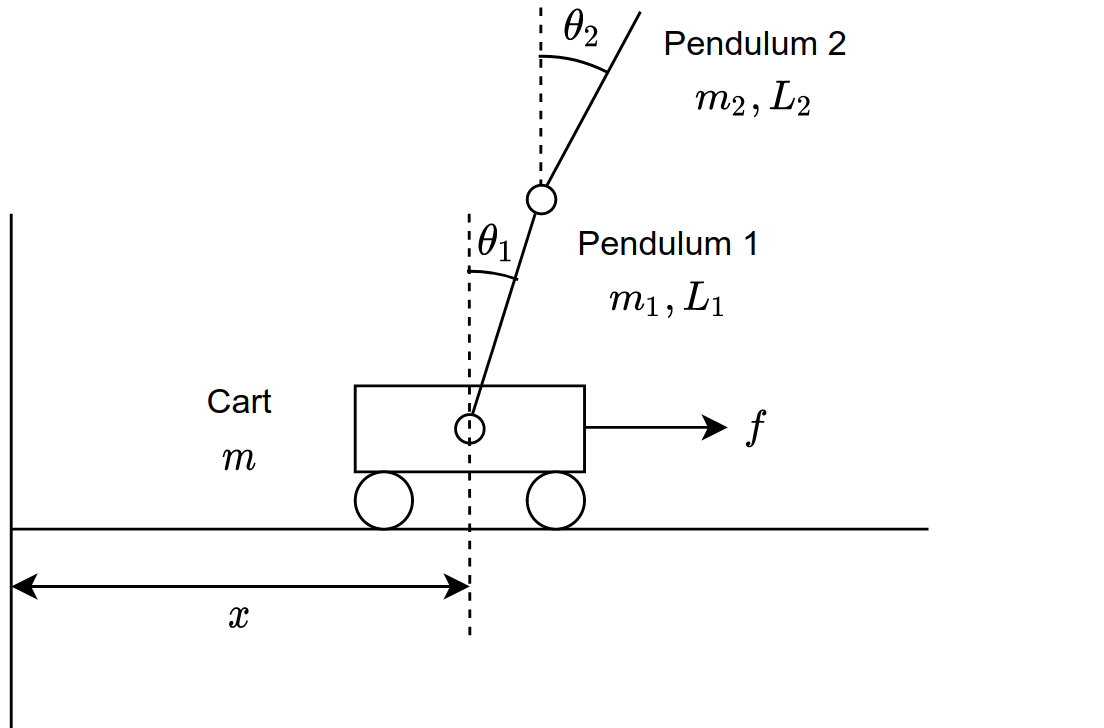
\includegraphics[width=2.5in]{fig01_cart001.png}
    \caption{Physical System}
    \label{fig:cart}
\end{figure}


\subsection{State Definition}
Suppose we have a continuous-time, nonlinear system presented in state space
form.  q is the state vector and has 3x1 dimensions. Function f is the
state transition function and u is the input to the system. Function h is the
state observation function.

\begin{equation}
    % \label{eq:6}
    \dot{q} = f(q,u),
\end{equation}
\begin{equation}
% \label{eq:7}
    y = h(q).
\end{equation}


Our goal is to stabilize the pendulums in the upright position and with the
pendulum angles close to zero.

\subsection{Noise and Friction}
To keep the project simple, noise is neglected but in reality there are always
multiple types of noise observed in measurement. Since we are using a simulation
environment there is no noise but the system still behaves chaotically. Friction
and damping terms are represented in the dynamic model with linear ansatz.

\subsection{Global Coordinate Frame}
We need to form a homogenous configuration space to present state variables
\(x, \theta_1, \theta_2\). We this global coordinate frame by defining the
following relative transforms. We assume \(q(t=0)\) is at the origin at the start
of the simulation.
\begin{equation}
    \begin{split}
    % \label{eq:6}
    x = \begin{bmatrix}
    x \\
    0 \\
    \end{bmatrix}, ~~
    q_1 = \begin{bmatrix}
    x + l_1 \sin \theta_1 \\
    l_1 \cos \theta_1 \\
    \end{bmatrix}, \\
    % \label{eq:6}
    q_2 = \begin{bmatrix}
    x + l_1 \sin \theta_1 + l_2 \sin \theta_2 \\
    l_1 \cos \theta_1 + l_2 \cos \theta_2 \\
\end{bmatrix},
\end{split}
\end{equation}
\noindent
We denote position of point-masses for \(m_c\), \(m_1\), and
\(m_2\) by \(x, q_1, q_2 \in R^2\) on the x-y plane.
We seek to define our system in terms of these state variables. Thus, we define
state variable vector \(q(t)\) as
\begin{equation}
q = [x, q_1, q_2]^{T}
\end{equation}

For simpler representation, we denote time-dependant state variable vector
as \(q:=q(t)\).


\section{Euler-Lagrangian Model}


\subsection{Equations of Motion}
Per \emph{Lagrangian mechanics}; first we derive the \emph{equations of motion}
by modeling of the physical system and find the \emph{Lagrangian}, \(\mathcal{L}= K -P\). \(K\) and \(P\) represent
\emph{kinetic} and \emph{potential} energies of the system. \(K\) is the total
kinetic energy from all three masses. Here, we define K as
\begin{equation}
    K = \frac{1}{2} m v^2 =~ \frac{1}{2} {m_c\|\dot{x}\|^2 + m_1\|\dot{q_1}\|^2 + m_2\|\dot{q_2}\|^2}.
\end{equation}

P denotes the overall potential energy of the system; but since the cart rolls
flat along the x-axis, it is inherently incapable of storing energy so we discard
it. P is obtained by
\begin{equation}
    P = g \left[ m_1 l_1 \cos \theta_1 + m_2 (l_1 \cos \theta_1 + l_2 cos \theta_2) \right]
\end{equation}
Where \(g \in R\) denotes gravitational acceleration.
Next, we use the \emph{Euler-Lagrange} equation to write the following ODE system.

\emph{The Lagrange Equations of Motions} are defined as
\begin{equation}
    Q = \frac{\partial\mathcal{L}}{\partial f_{i}} - \frac{d}{dt} \left( \frac{\partial \mathcal{L}}{\partial f_{i}}\right).
\end{equation}
Where \(Q\) represents the vector of sum of external forces acting on the plan.
We solve for an \emph{linearized} solution by setting Q to zero. This is also
called the \emph{zero dynamics} of the system.

\begin{equation}
    \mathcal{L} = \mathcal{L}(t, q, \dot{q})
\end{equation}
\begin{equation}
\begin{cases}
\begin{array}{rcl}
    u -d_1 \dot{q} &=& \frac{d}{dt} \{\frac{\partial\mathcal{L}}{\partial\dot{q}}\}-\{\frac{\partial\mathcal{L}}{\partial q}\}\\
    -d_2 \dot{\theta_1} &=& \frac{d}{dt} \{\frac{\partial\mathcal{L}}{\partial\dot{\theta_1}}\}-\{\frac{\partial\mathcal{L}}{\partial \theta_1}\}\\
    -d_3 \dot{\theta_2} &=& \frac{d}{dt} \{\frac{\partial\mathcal{L}}{\partial\dot{\theta_2}}\}-\{\frac{\partial\mathcal{L}}{\partial \theta_2}\}\\
    \end{array}
\end{cases}
\end{equation}

So far our derivation has made our expressions more complicated but these steps are
necessary for capturing the full dynamic characteristics of the system. In the
following section, we linearize the continuous-time nonlinear model about the
upright position.

\subsection{Continues-Time, Nonlinear Model}
We used MATLAB Symbolic Math Toolbox to derive the resultant ODE. Obtaining
symbolic or implicit expressions of our ODE will allow us to model a general
DIP system.

\begin{equation}
\text{\scriptsize $
% \begin{cases}
\begin{array}{rcl}
    u -d_1 \dot{q} &=& (m_c+m_1+m_2)\ddot{q}+l_1(m_1+m_2)\ddot{\theta_1} \cos \theta_1\\
    & & + m_2 l_2 \ddot{\theta_2} \cos \theta_2 - l_1 (m_1+m_2) \dot{\theta_1}^2 \sin \theta_1 \\
    & & - m_2 l_2 \dot{\theta_2}^2 \sin \theta_2\\
    -d_2 \dot{\theta_1} &=& l_1 (m_1+m_2) \ddot(q) \cos \theta_1
    +l_1^2 (m_1+m_2) \ddot{\theta_1}\\
    & & +l_1 l_2 m_2 \ddot{\theta_2} \cos (\theta_1 - \theta_2)+ l_1 l_2 m_2 \dot{\theta_2}^2 \sin(\theta_1 - \theta_2) \\
    & & - g(m_1+m_2) l_1 \sin \theta_1 \\
    -d_3 \dot{\theta_2} &=& l_2 m_2 \ddot{q} \cos \theta_2
    + l_1 l_2 m_2 \ddot{\theta_1} \cos (\theta_1 -\theta_2)
    + l_2^2 m_2 \ddot{\theta_2}\\
    & & -l_1 l_2 m_2 \dot{\theta_1}^2 \sin (\theta_1 - \theta_2)
    - l_2 m_2 g \sin \theta_2\\
    \end{array}
% \end{cases}
$}
\end{equation}

% \subsection{Optimal Control}
% define
% in other words
% so we do this

\subsection{Linearization}
First, we rewrite the equations of motion into matrix form to batch acceleration,
velocity, and position terms into separate matrices. A second order representation
of the physical system is sufficient to provide an accurate enough estimate,
per \emph{Taylor Series Linearization} method. This is an important step as
identifying system dynamics lies at the heart of \emph{Optimal Control}.
\begin{equation}
D(q) \ddot{q} + C(q, \dot{q}) \dot{q} + G(q) = Hu
\end{equation}
where matrix functions \(D(q) \ddot{q} + C(q, \dot{q}) \dot{q} + G(q)\)
represent systems dynamics with respect to time,
current state and previous state. Time variable \(t\) is omitted to simplify
notation. The system energy state (left hand side of
above EOM) is presented in relation to external forces \(Hu\) acting on the
system. Vector \(u \in R^1\) represents external input forces vector and matrix
\(H\) represents its relationship with state variable functions. Matrix
functions \(D(q),~C(q, \dot{q}),~G(q)\) and vector H are define as presented in
\cite{optimalLQR}.

We need to rewrite the EOM in the following
matrix form to obtain the final ODE. Per \emph{Lyapunov
Control Function theory} (LCF) for autonomous dynamical systems and
\emph{LaSalle's}, we can assume there exists a
\emph{Optimal Control Trajectory} or \emph{Hamiltonian Flow} for a valid
initial condition if the LCF is a \emph{positive definite} and \emph{positive
semi-definite} energy function.
Moreover, the energy function describing the system must be \emph{symmetric} and \emph{positive definite} in order to form \emph{stable} control trajectory.

\begin{equation}
M(q)\dot{q} = A(q)q + Bu
\end{equation}

Where \emph{positive definite} or \emph{positive semi-definite} constraints are
evaluated by computing the determinant of \(M\).
\begin{equation}
det(M) > 0;~ \forall q
\end{equation}
Such that, the final ODE can be written as
\begin{equation}
    \dot{q} = M(q)^{-1}(A(q)q + Bu)
\end{equation}

where A and B are defined as
\begin{equation}
    A =
\begin{bmatrix}
        0 & I \\
        D(^{-1} \frac{\partial G}{\partial q} & 0 \\
\end{bmatrix}
\end{equation}

\begin{equation}
    B =
\begin{bmatrix}
    0 \\
    D^{-1} H\\
    \end{bmatrix}
    \end{equation}


\subsection{Linear Quadratic Regulator Solution}
So far, we have modeled, linearized, and discretized our system using state
space general form. In the process, we systematically reduced the solution space
complexity by replacing time \(t\) and velocity dimension as linear products of
current and previous states. This allows us to analytically derive a general
form optimal solution. But before we reach that step, we need to define a
general \emph{Cost Function} \(J\) that only depends on absolute minimal parameters,
which we will later optimize to arrive to a \emph{minimal surface}. Quadratic
performance index \(J \) is
defined as
\begin{equation}
J(x,u) = \frac{1}{2}x^{T}Q x + \frac{1}{2}u^{T}Ru
\end{equation}
whose solution is the minimal cost or minimum-energy input required for the
system to reach local minima, for any given initial state. Next, we minimize \(J\)
which will yield the state feedback weight vector \(K\) and is obtained by
recursively solving the dynamic \emph{Riccati} equation.
It is important to note that calculation of Quadratic losses are carried out by
performing dot product of state vector with its transpose and energy magnitude.



\section{Experiments}
A series of 18 tests are performed to investigate nonlinearities and stability
of the mentioned DIP system with a linear closed-loop feedback controller. The
tests are divided to two experiments; \emph{experiment I} investigates system
dynamics and LQR stability, given tuned and untuned control vector (eigenvalues),
\emph{experiment II} investigates the chaotic nature of the system. Moreover, a
brief description of the simulation and animation implementation is provided.


\begin{figure}
\centering
\subfigure[\(q(t)\)]{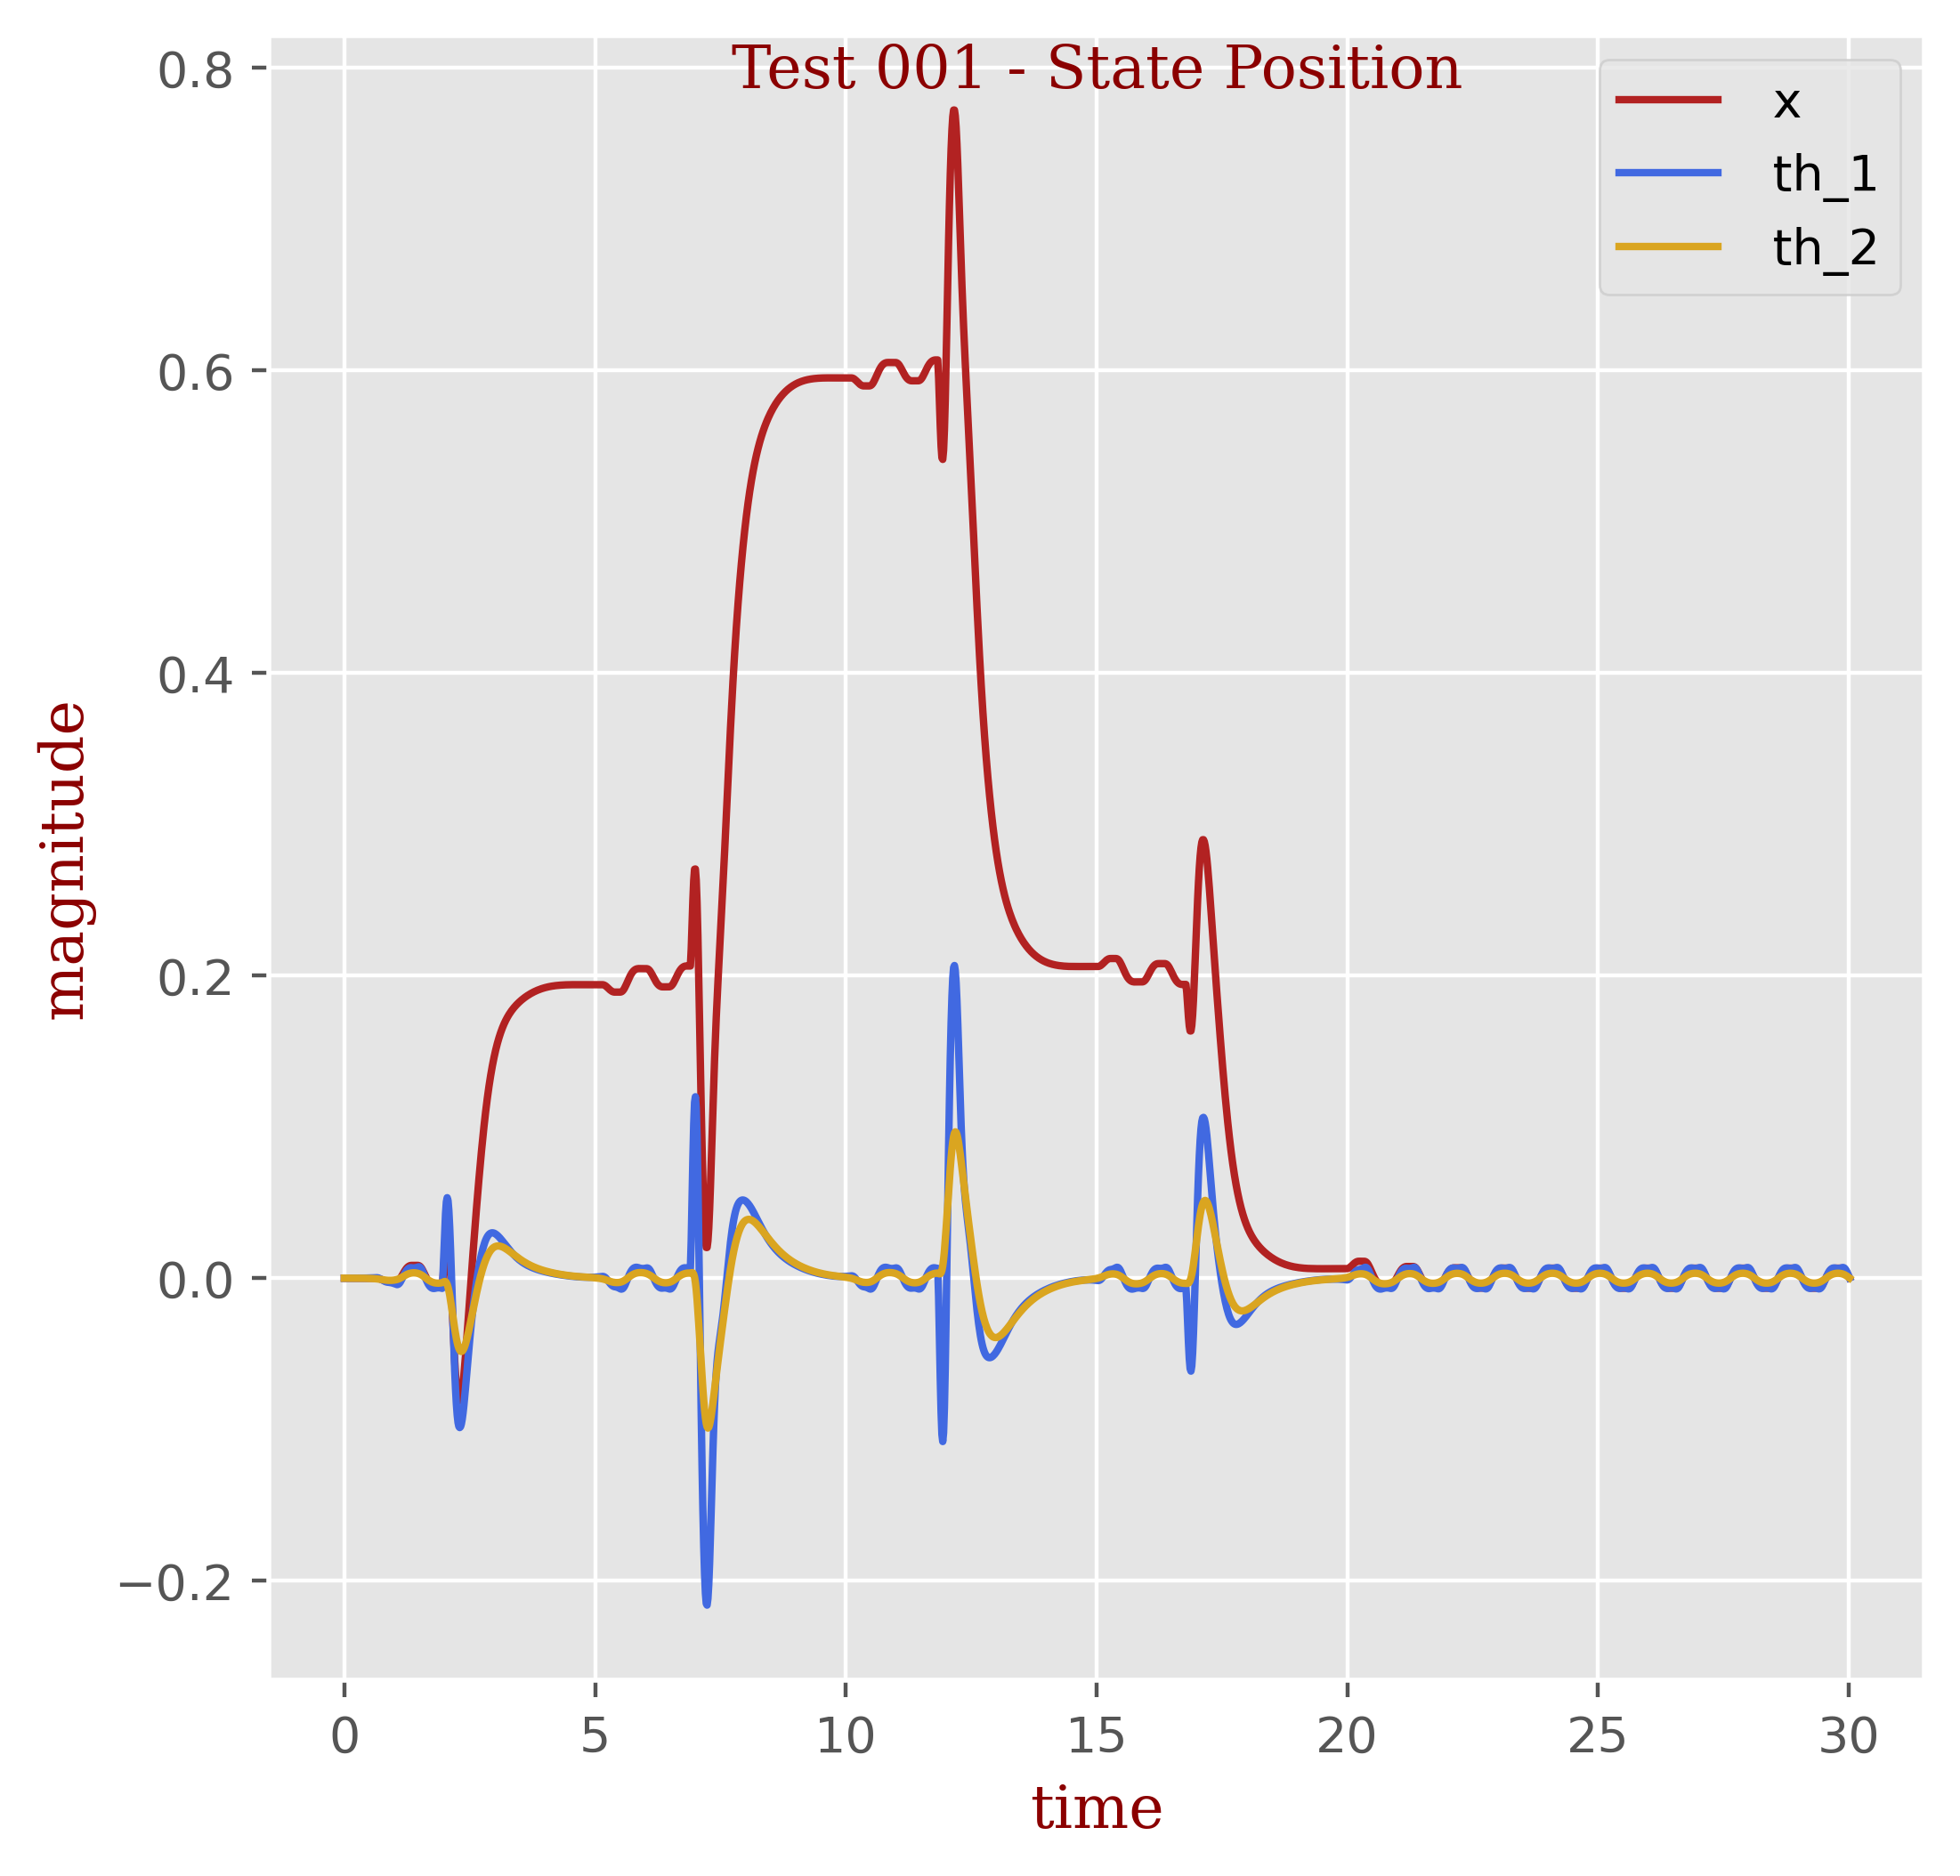
\includegraphics[width=27mm]{Test 001_State_Position.png}}
\subfigure[\(\dot{q}(t)\)]{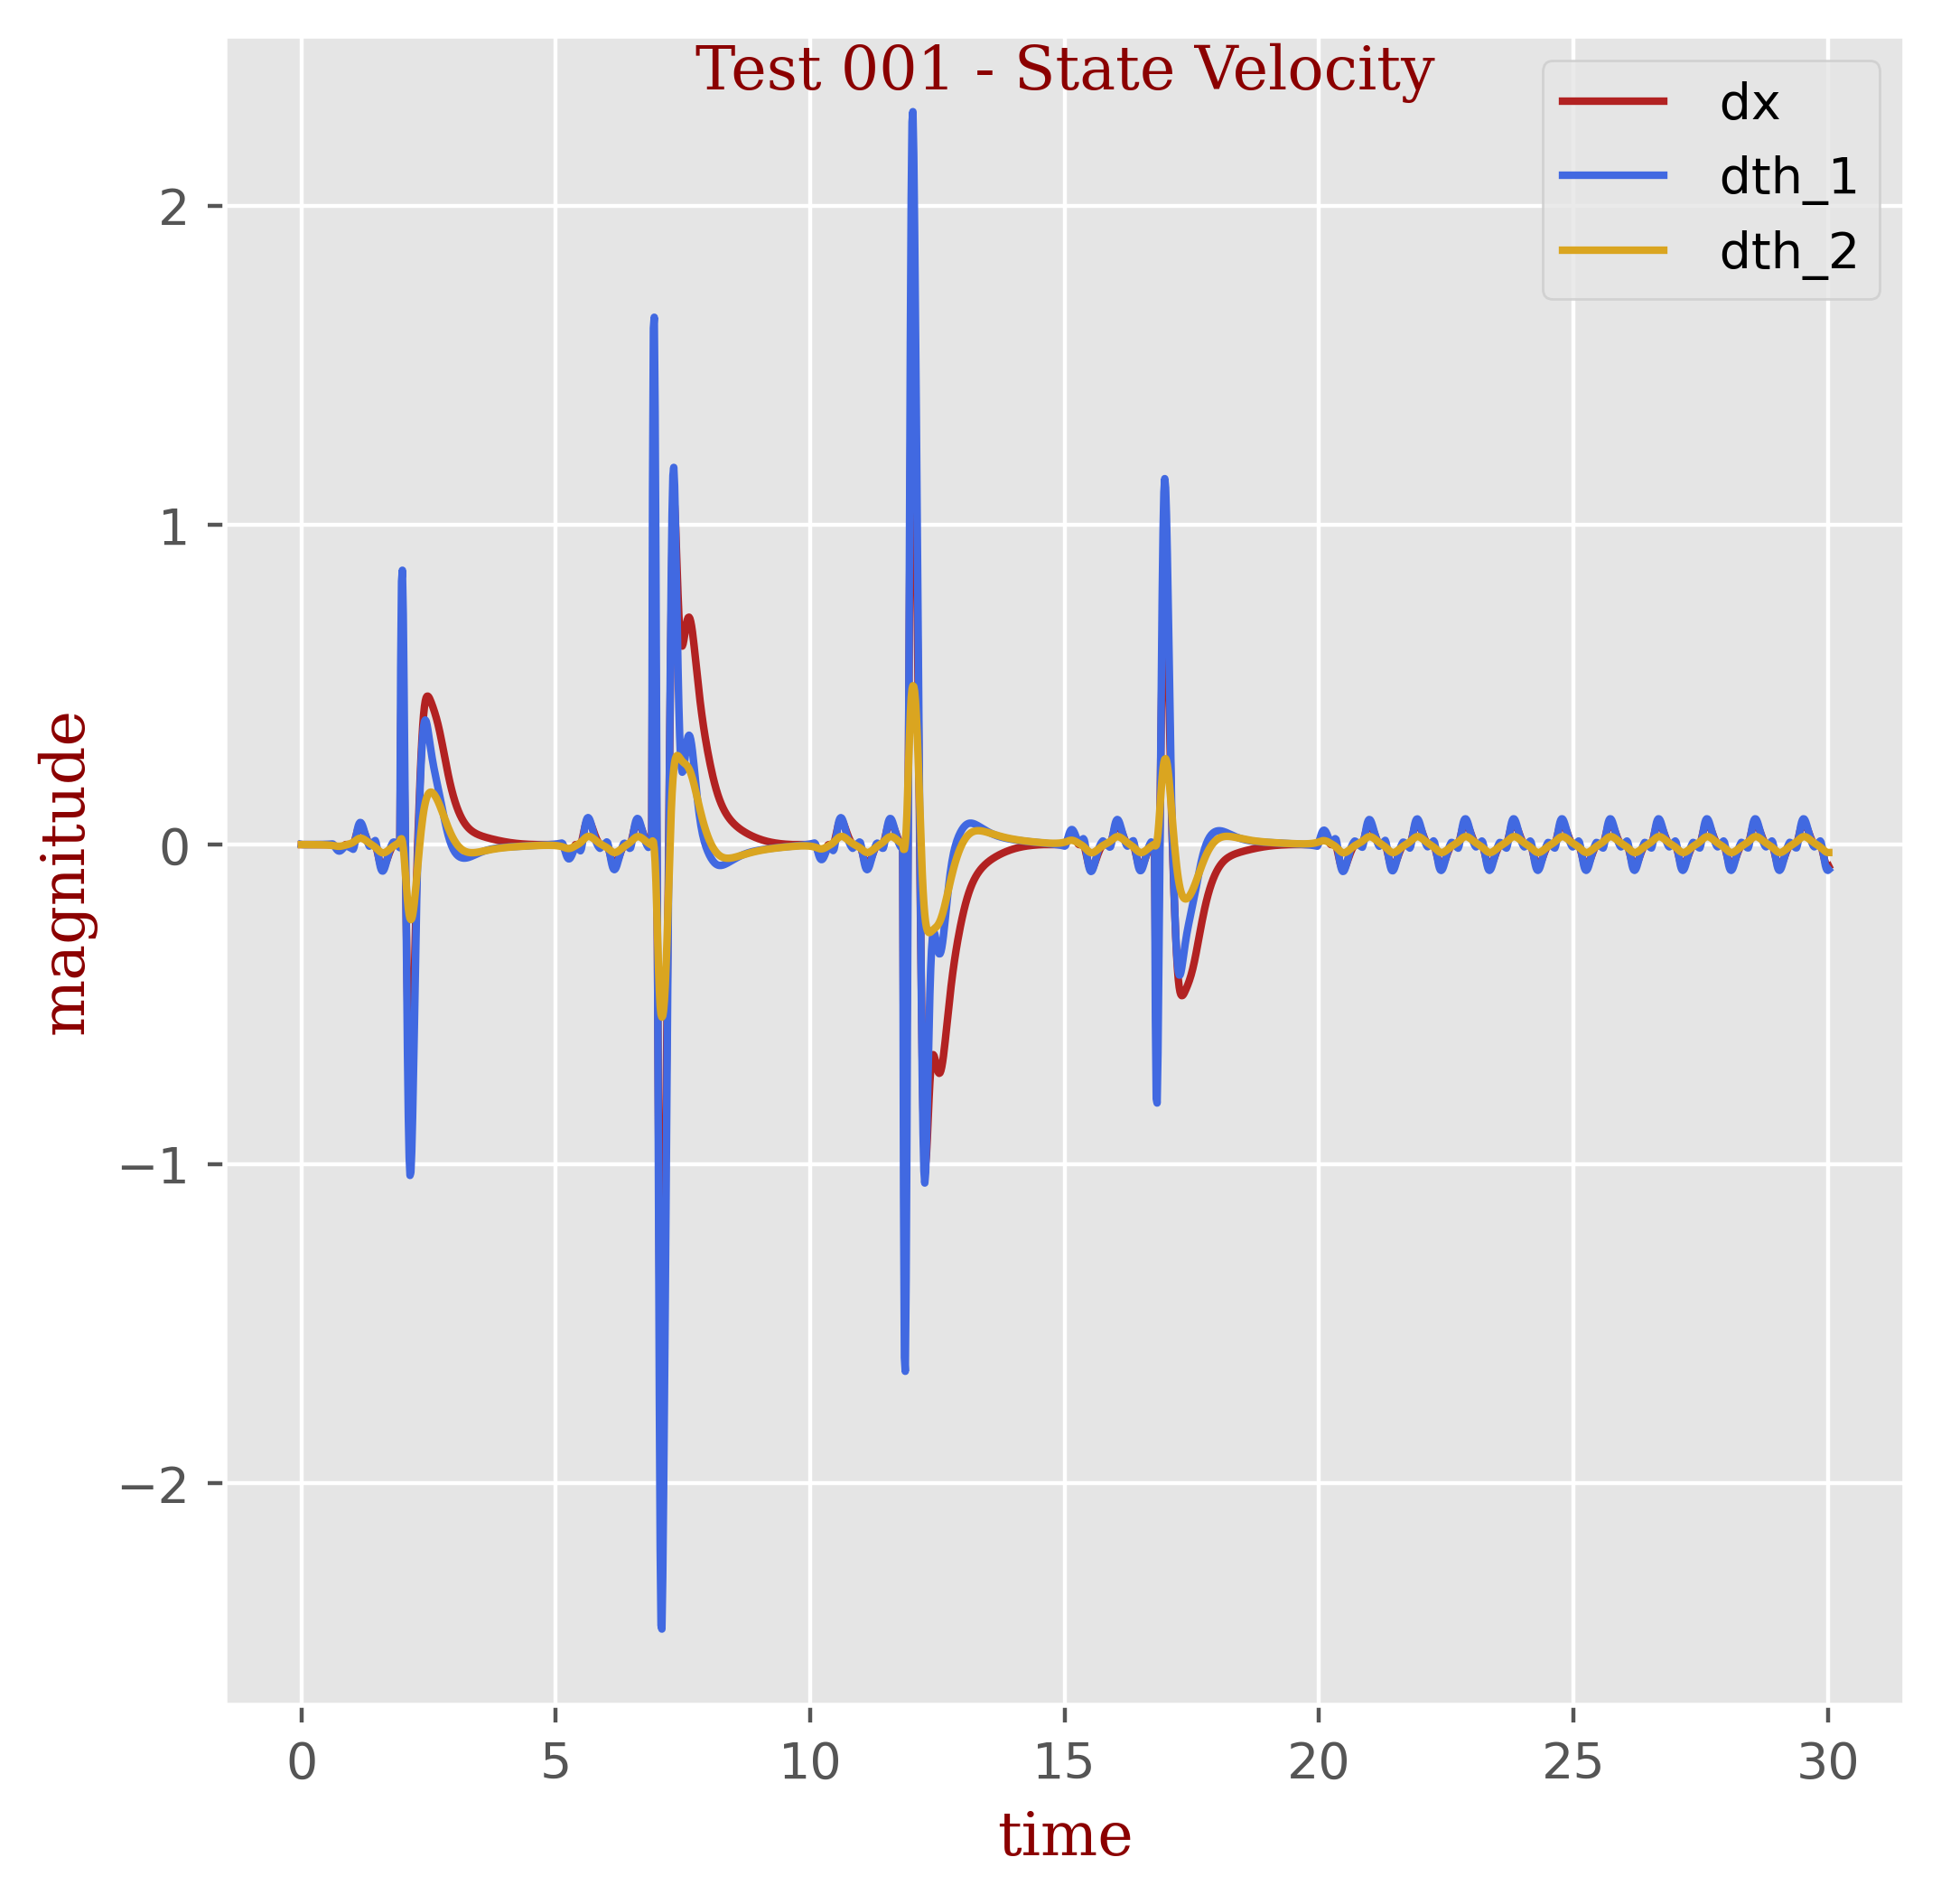
\includegraphics[width=27mm]{Test 001_State_Velocity.png}}
\subfigure[\(J(t)\)]{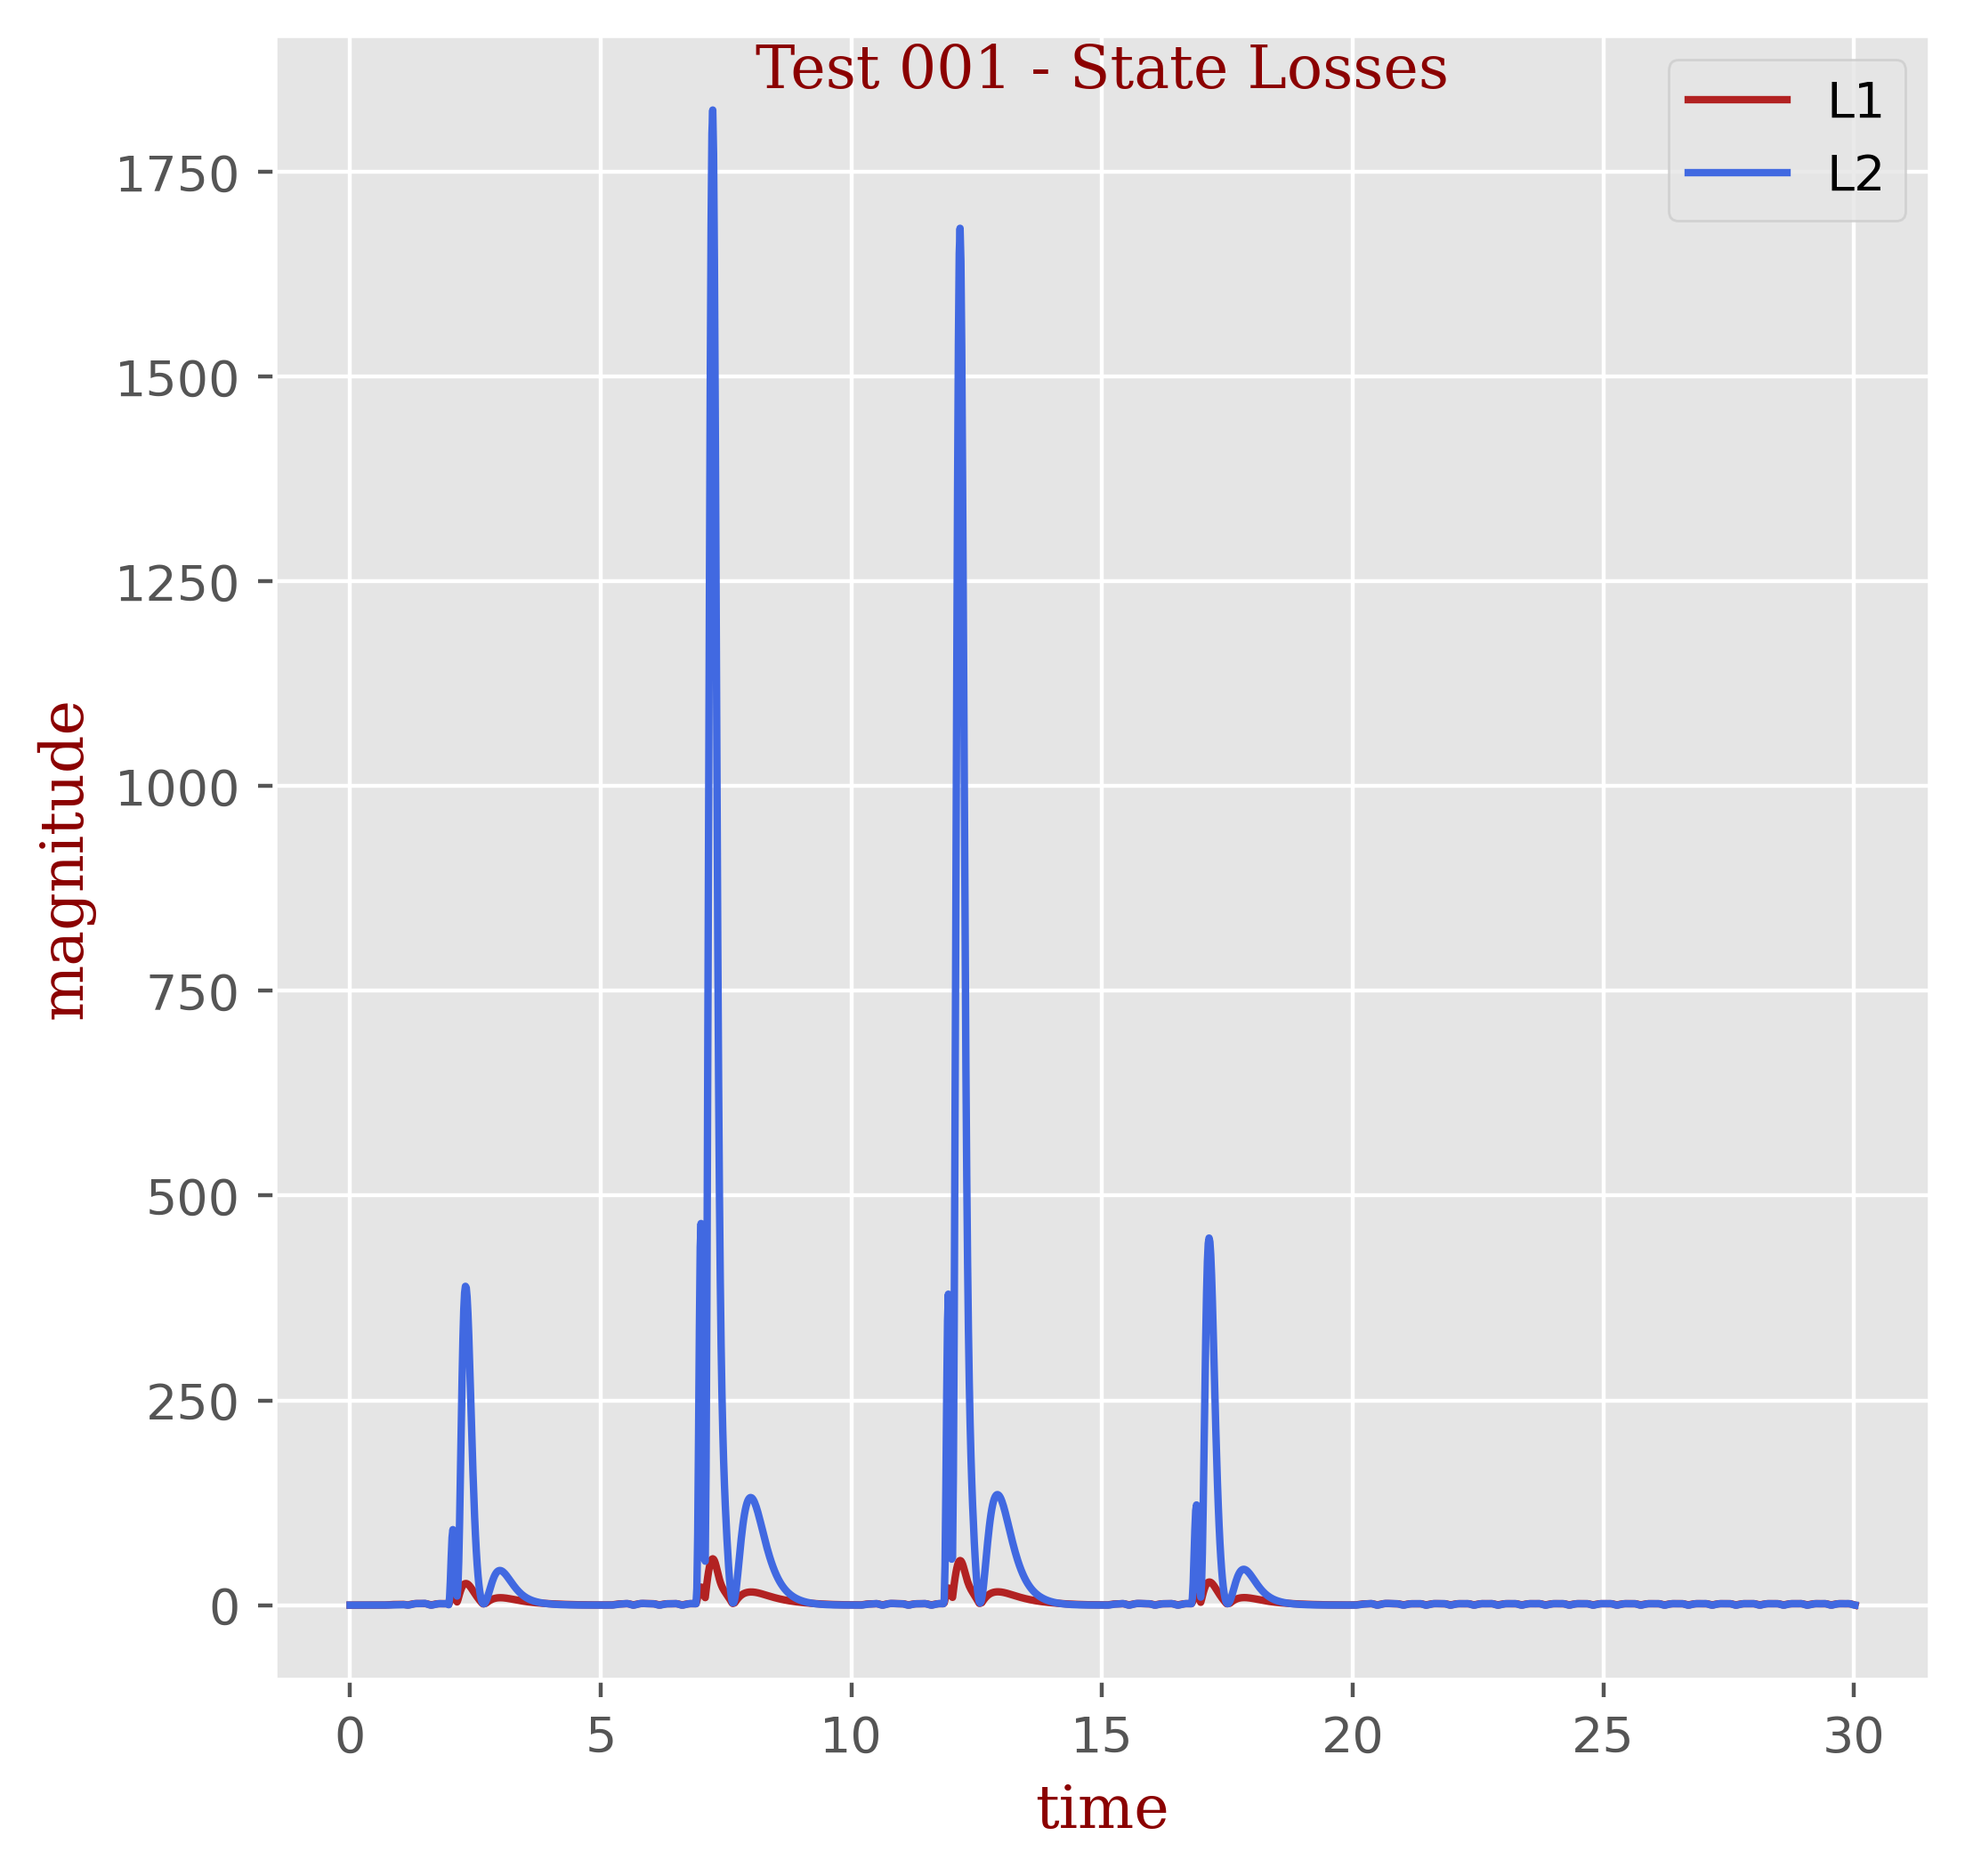
\includegraphics[width=27mm]{Test 001_State_Losses.png}}
\caption{Test 001}
\label{fig:t001}
\end{figure}


Each test was simulated and animated in real-time to ensure both validity and
diversity of tests for both experiments. Moreover, for each test the simulation
and controller data, L1 and L2 losses, and all relevant test configurations
are systematically captured and stored under \texttt{out} and \texttt{config}
directories on the provided repository. The data for each test is analyzed and
presented by 3 plots, \emph{state position}, \emph{state velocity}, and
\emph{state losses}. Test 001, figure \ref{fig:t001}, is the control for all tests
performed in both experiments. Control vector K used in all experiments are
tuned using \texttt{lyap()} function from MATLAB and parameters from Test 001
configuration were used.

It is important to note that, in order to construct a more appropriate analytic tools,
we decided to convert radians to degrees and omit cart position values when computing
post-precessing loss functions. This is not to be confused with the LQR solution
which uses quadratic errors (similar to L2). The reason for changing from radians
to degrees is that, for small changes (less than 1) a quadratic loss function
quadratically decreases the magnitude instead of increasing it.



\begin{figure}[!t]
    \centering
    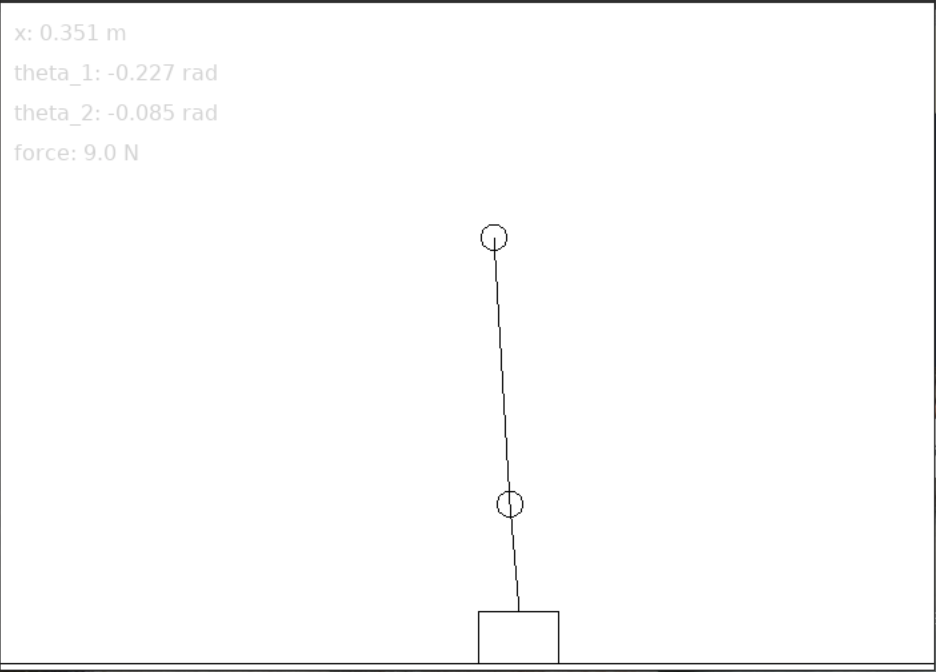
\includegraphics[width=2.5in]{fig_000_anim.png}
    \caption{Animation of Double Inverted Pendulum}
    \label{fig_000_anim}
\end{figure}


\subsection{Simulation and Animation}
For this project, both MATLAB and Python were used at different stages of the
development. Besides symbolic math derivation, MATLAB Control Toolbox was used
to check Python ODE simulation output and to obtain the LQR solution. MATLAB is
the gold-standard of scientific numerical analysis and Python is versaltile and
rich with high level feature. Various Python-based control system libraries were
explored and considered but were abandoned after observing variations in the
\emph{control vector} parameters. The LQR solution is expected to be optimal for
\emph{Lyapunov energy systems} and variations in the solution raises doubts
about numerical integrity of the computation process. For that reason, derivations
and control solutions used in this work are consistent with MATLAB.\\
Various Python libraries are used to simulate, animate and analyze model dynamics.
Pymunk and Pygame libraries are used create a 2D physics-based simulation
environment. Pyglet library (based on OpenGL) is used to create the animation,
figure \ref{fig_000_anim}. Source code for the animation and graphics are base
on examples and documentation provided by the authors \cite{pymunk} \cite{pygame}.



\subsection{Experiment I}
In the first experiment, we perform a set of 14 tests with the goal of studying
system stability with respect to changes in model parameters.
The control vector,
K, obtained from MATLAB is tuned for model parameters used in Test 001 (figure
\ref{fig:t001}). This control vector is
used without retuning for all 14 tests in this experiment. Moreover, the duration of the test,
friction and initial momentums are 30s, 0.2, and 0.001\(N/m\), respectively. These
values remained the same for all 14 tests. We changed model parameters whose
dynamics play a dominant role in the overall system dynamics. Thus, model
parameters \(l_1\), \(m_1\), \(l_2\), and \(m_2\) were changed one at the time
to see how each affects system dynamics and controller stability.
Table 1 \ref{tab:001} presents model parameters used for each test and changes
from each test to the following is highlighted in \textbf{bold}.

\begin{table}[!t]
\renewcommand{\arraystretch}{1.3}
\caption{Experiment I}
\label{tab:001}
\centering
\begin{tabular}{|c||c|c|c|c|c|}
\hline
Test ID & \(l_1\) & \(m_1\) & \(l_2\) & \(m_2\) & stability \\
\hline\hline
001 & \textbf{0.6} & \textbf{0.2} & \textbf{0.6} & \textbf{0.2} & UUB\\
002 & 0.6 & \textbf{0.3} & 0.6 & 0.2 & UUB\\
003 & 0.6 & \textbf{0.4} & 0.6 & 0.2 & UUB\\
004 & 0.6 & 0.4 & 0.6 & \textbf{0.3} & UUB\\
005 & 0.6 & 0.4 & 0.6 & \textbf{0.4} & UUB\\
006 & 0.6 & \textbf{0.3} & 0.6 & 0.4 & UUB\\
007 & 0.6 & \textbf{0.2} & 0.6 & 0.4 & marginal-UUB\\
008 & 0.6 & 0.2 & \textbf{0.5} & 0.2 & unstable\\
009 & 0.6 & 0.2 & \textbf{0.7} & 0.2 & unstable\\
010 & 0.6 & 0.2 & \textbf{0.8} & 0.2 & unstable\\
011 & \textbf{0.5} & 0.2 & \textbf{0.6} & 0.2 & UUB\\
012 & \textbf{0.4} & 0.2 & 0.6 & 0.2 & UUB \\
013 & \textbf{0.3} & 0.2 & 0.6 & 0.2 & marginal-UUB\\
014 & \textbf{0.7} & 0.2 & 0.6 & 0.2 & unstable\\
\hline
\end{tabular}
\end{table}

Test 001 proves \emph{practical stability} of LQR solution obtained from MATLAB
by bounding \(\theta_1\) and \(\theta_2\) to small positive magnitude angle
close to zero degrees. There is no noise added to the simulation but quantization
error itself acts as process noise. This noise is significant enough to make the
simulated system behave chaotically similar to a physical system. We can only
achieve \emph{Uniformly Ultimately Bounded} (UUB) with a linear controller,
figure \ref{fig:t001}.



\begin{figure}
\centering
\subfigure[\(q(t)\)]{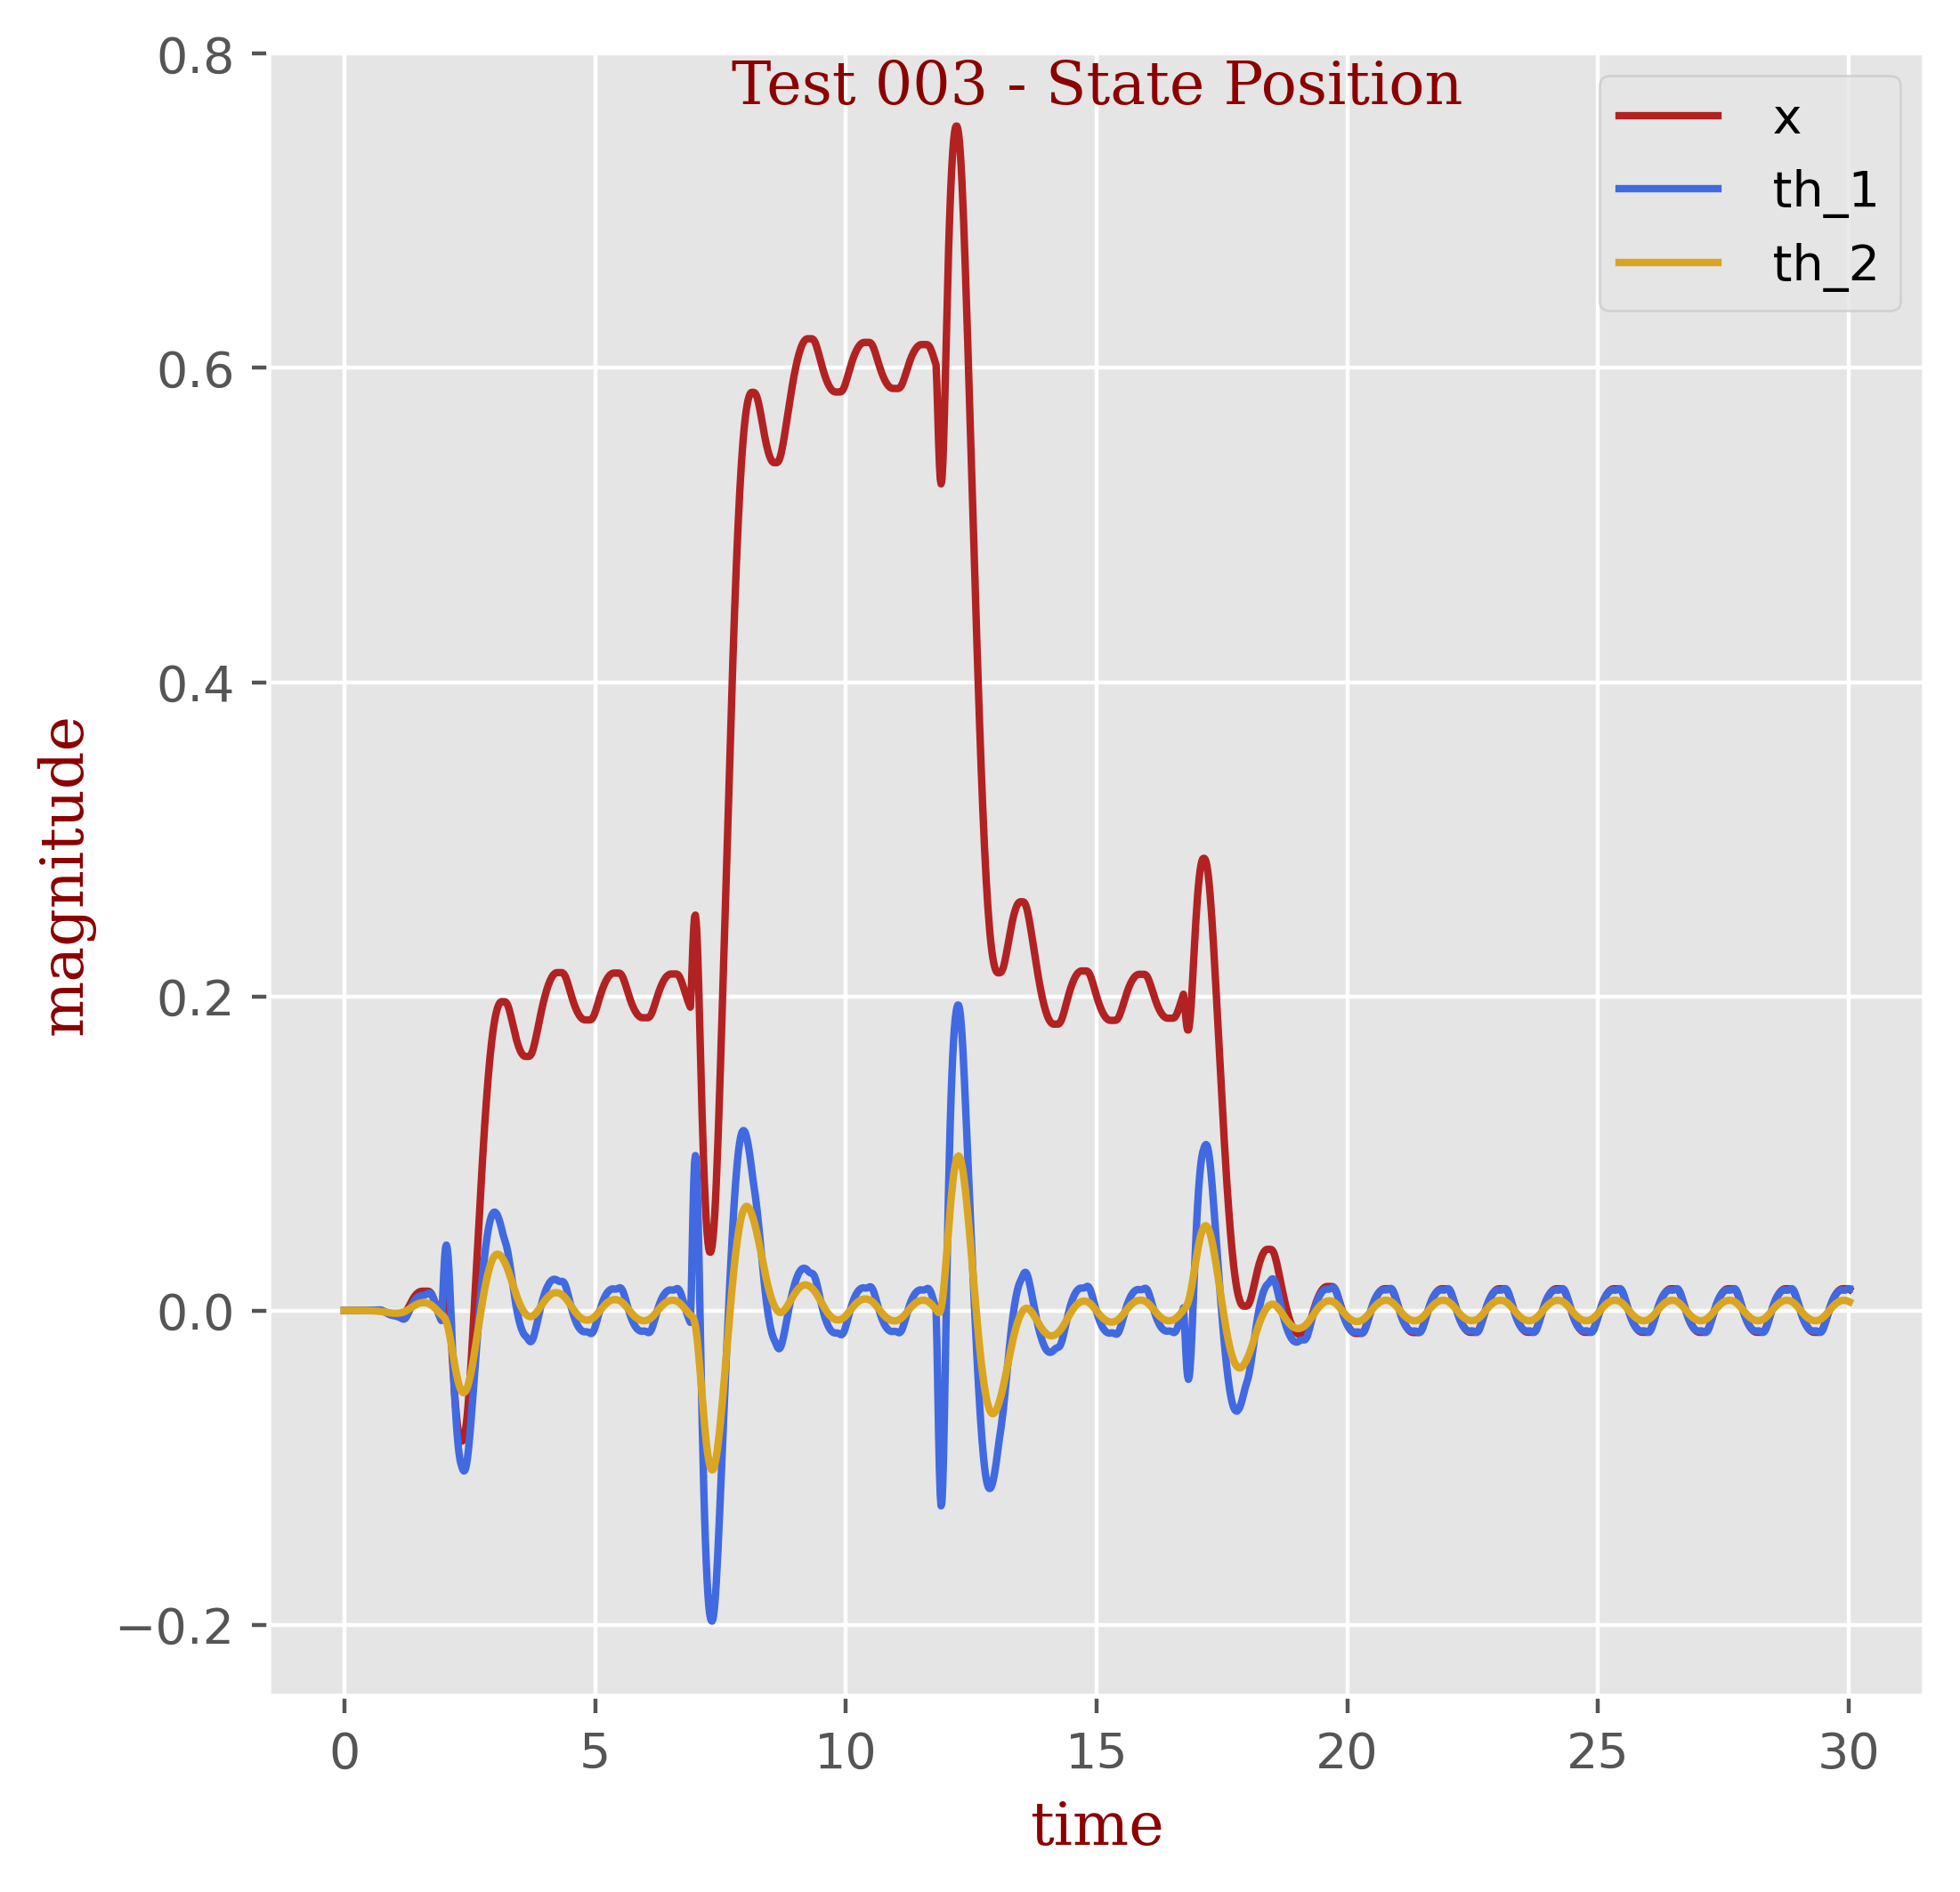
\includegraphics[width=27mm]{Test 003_State_Position.png}}
\subfigure[\(\dot{q}(t)\)]{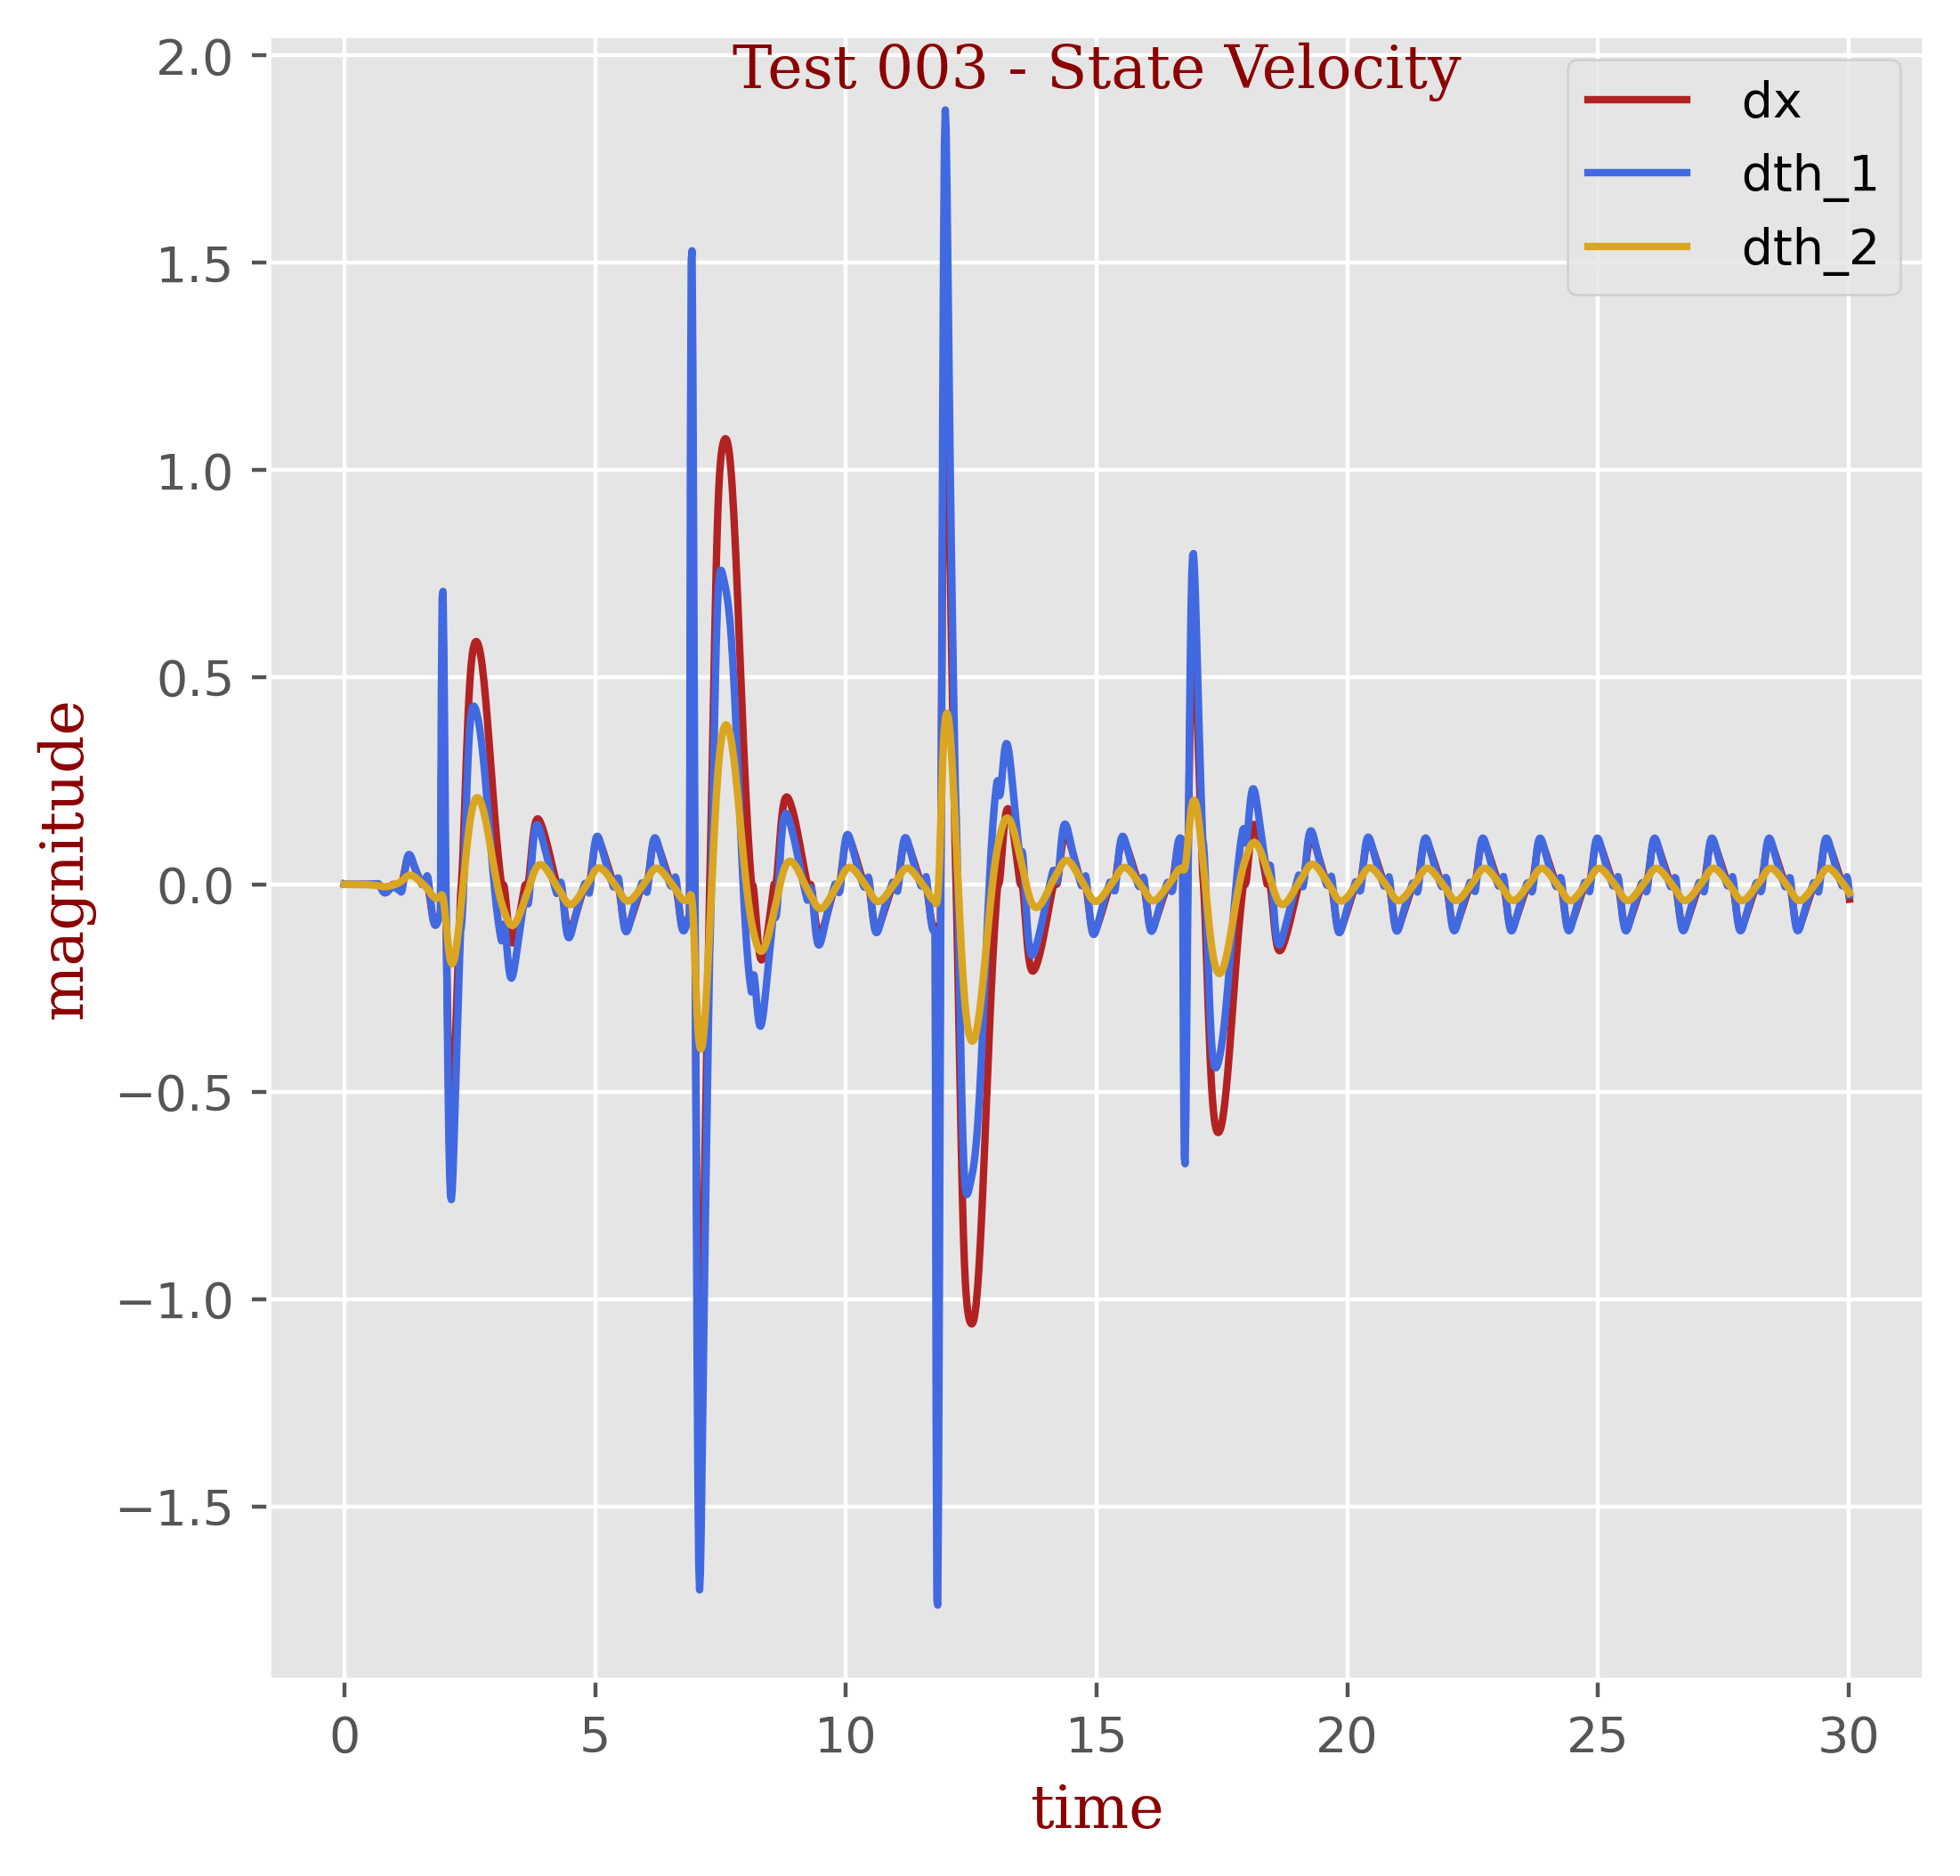
\includegraphics[width=27mm]{Test 003_State_Velocity.png}}
\subfigure[\(J(t)\)]{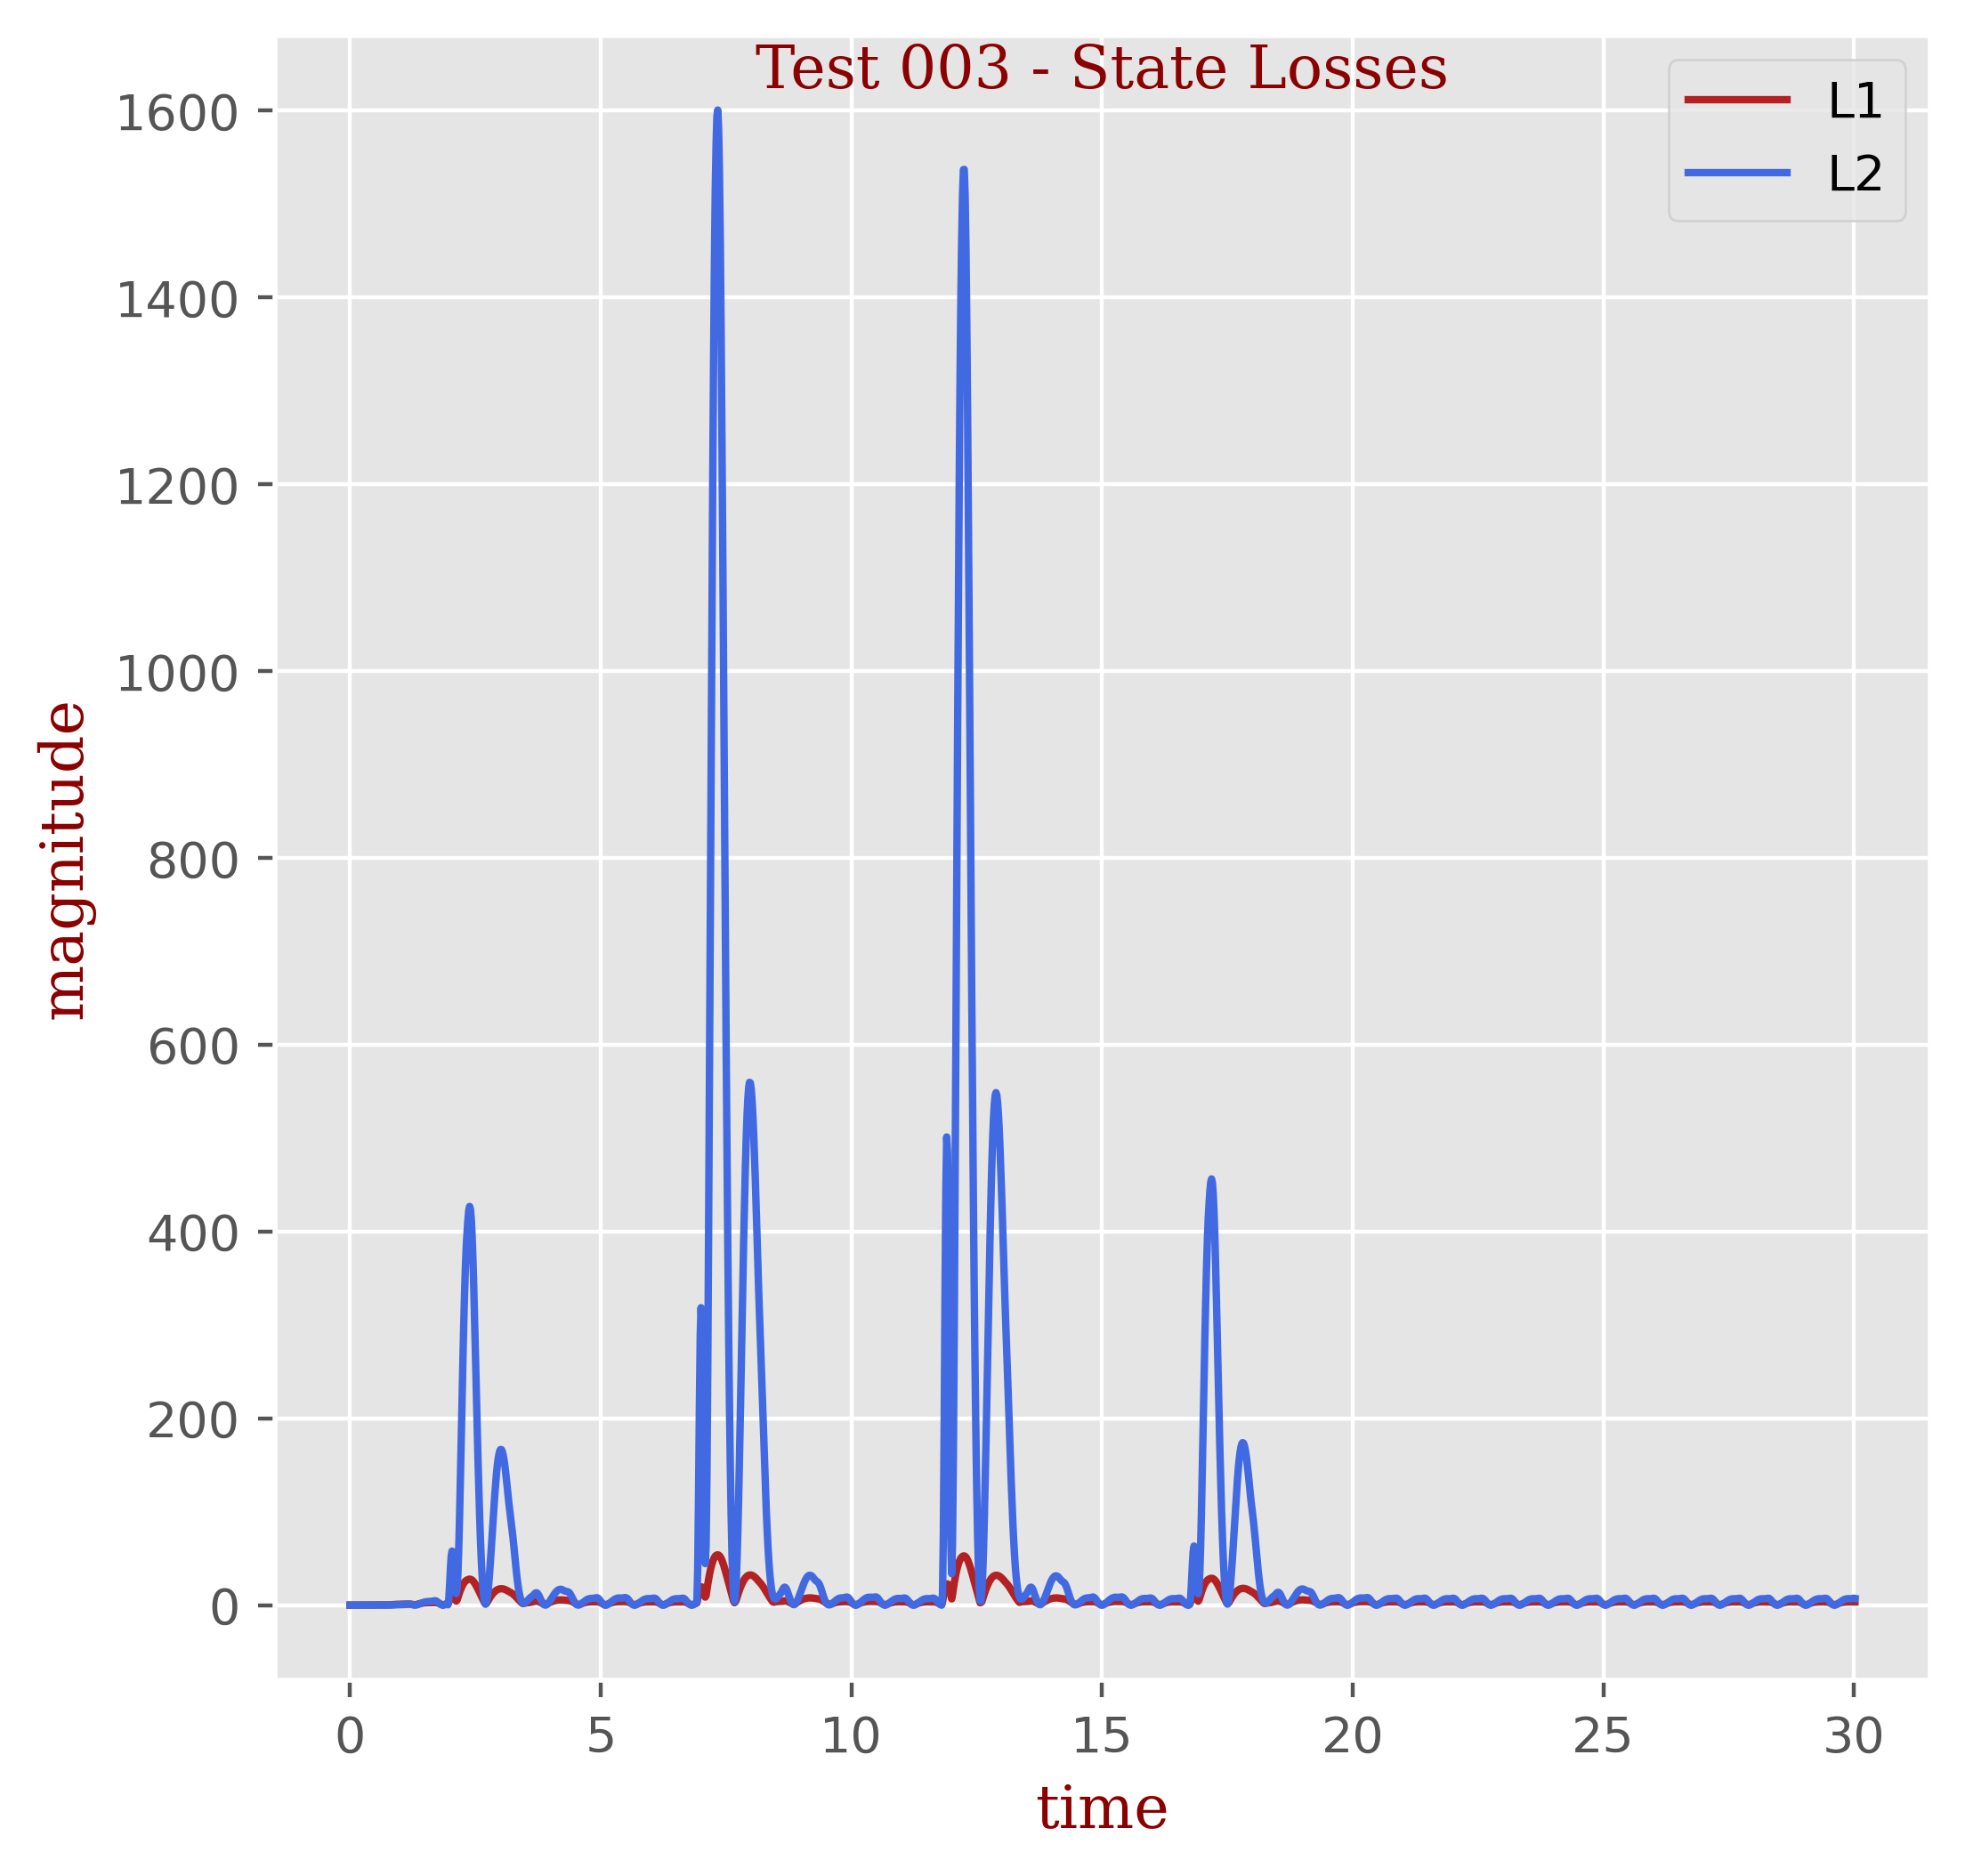
\includegraphics[width=27mm]{Test 003_State_Losses.png}}
\caption{Test 003}
\label{fig:t003}
\end{figure}

\begin{figure}
\centering
\subfigure[\(q(t)\)]{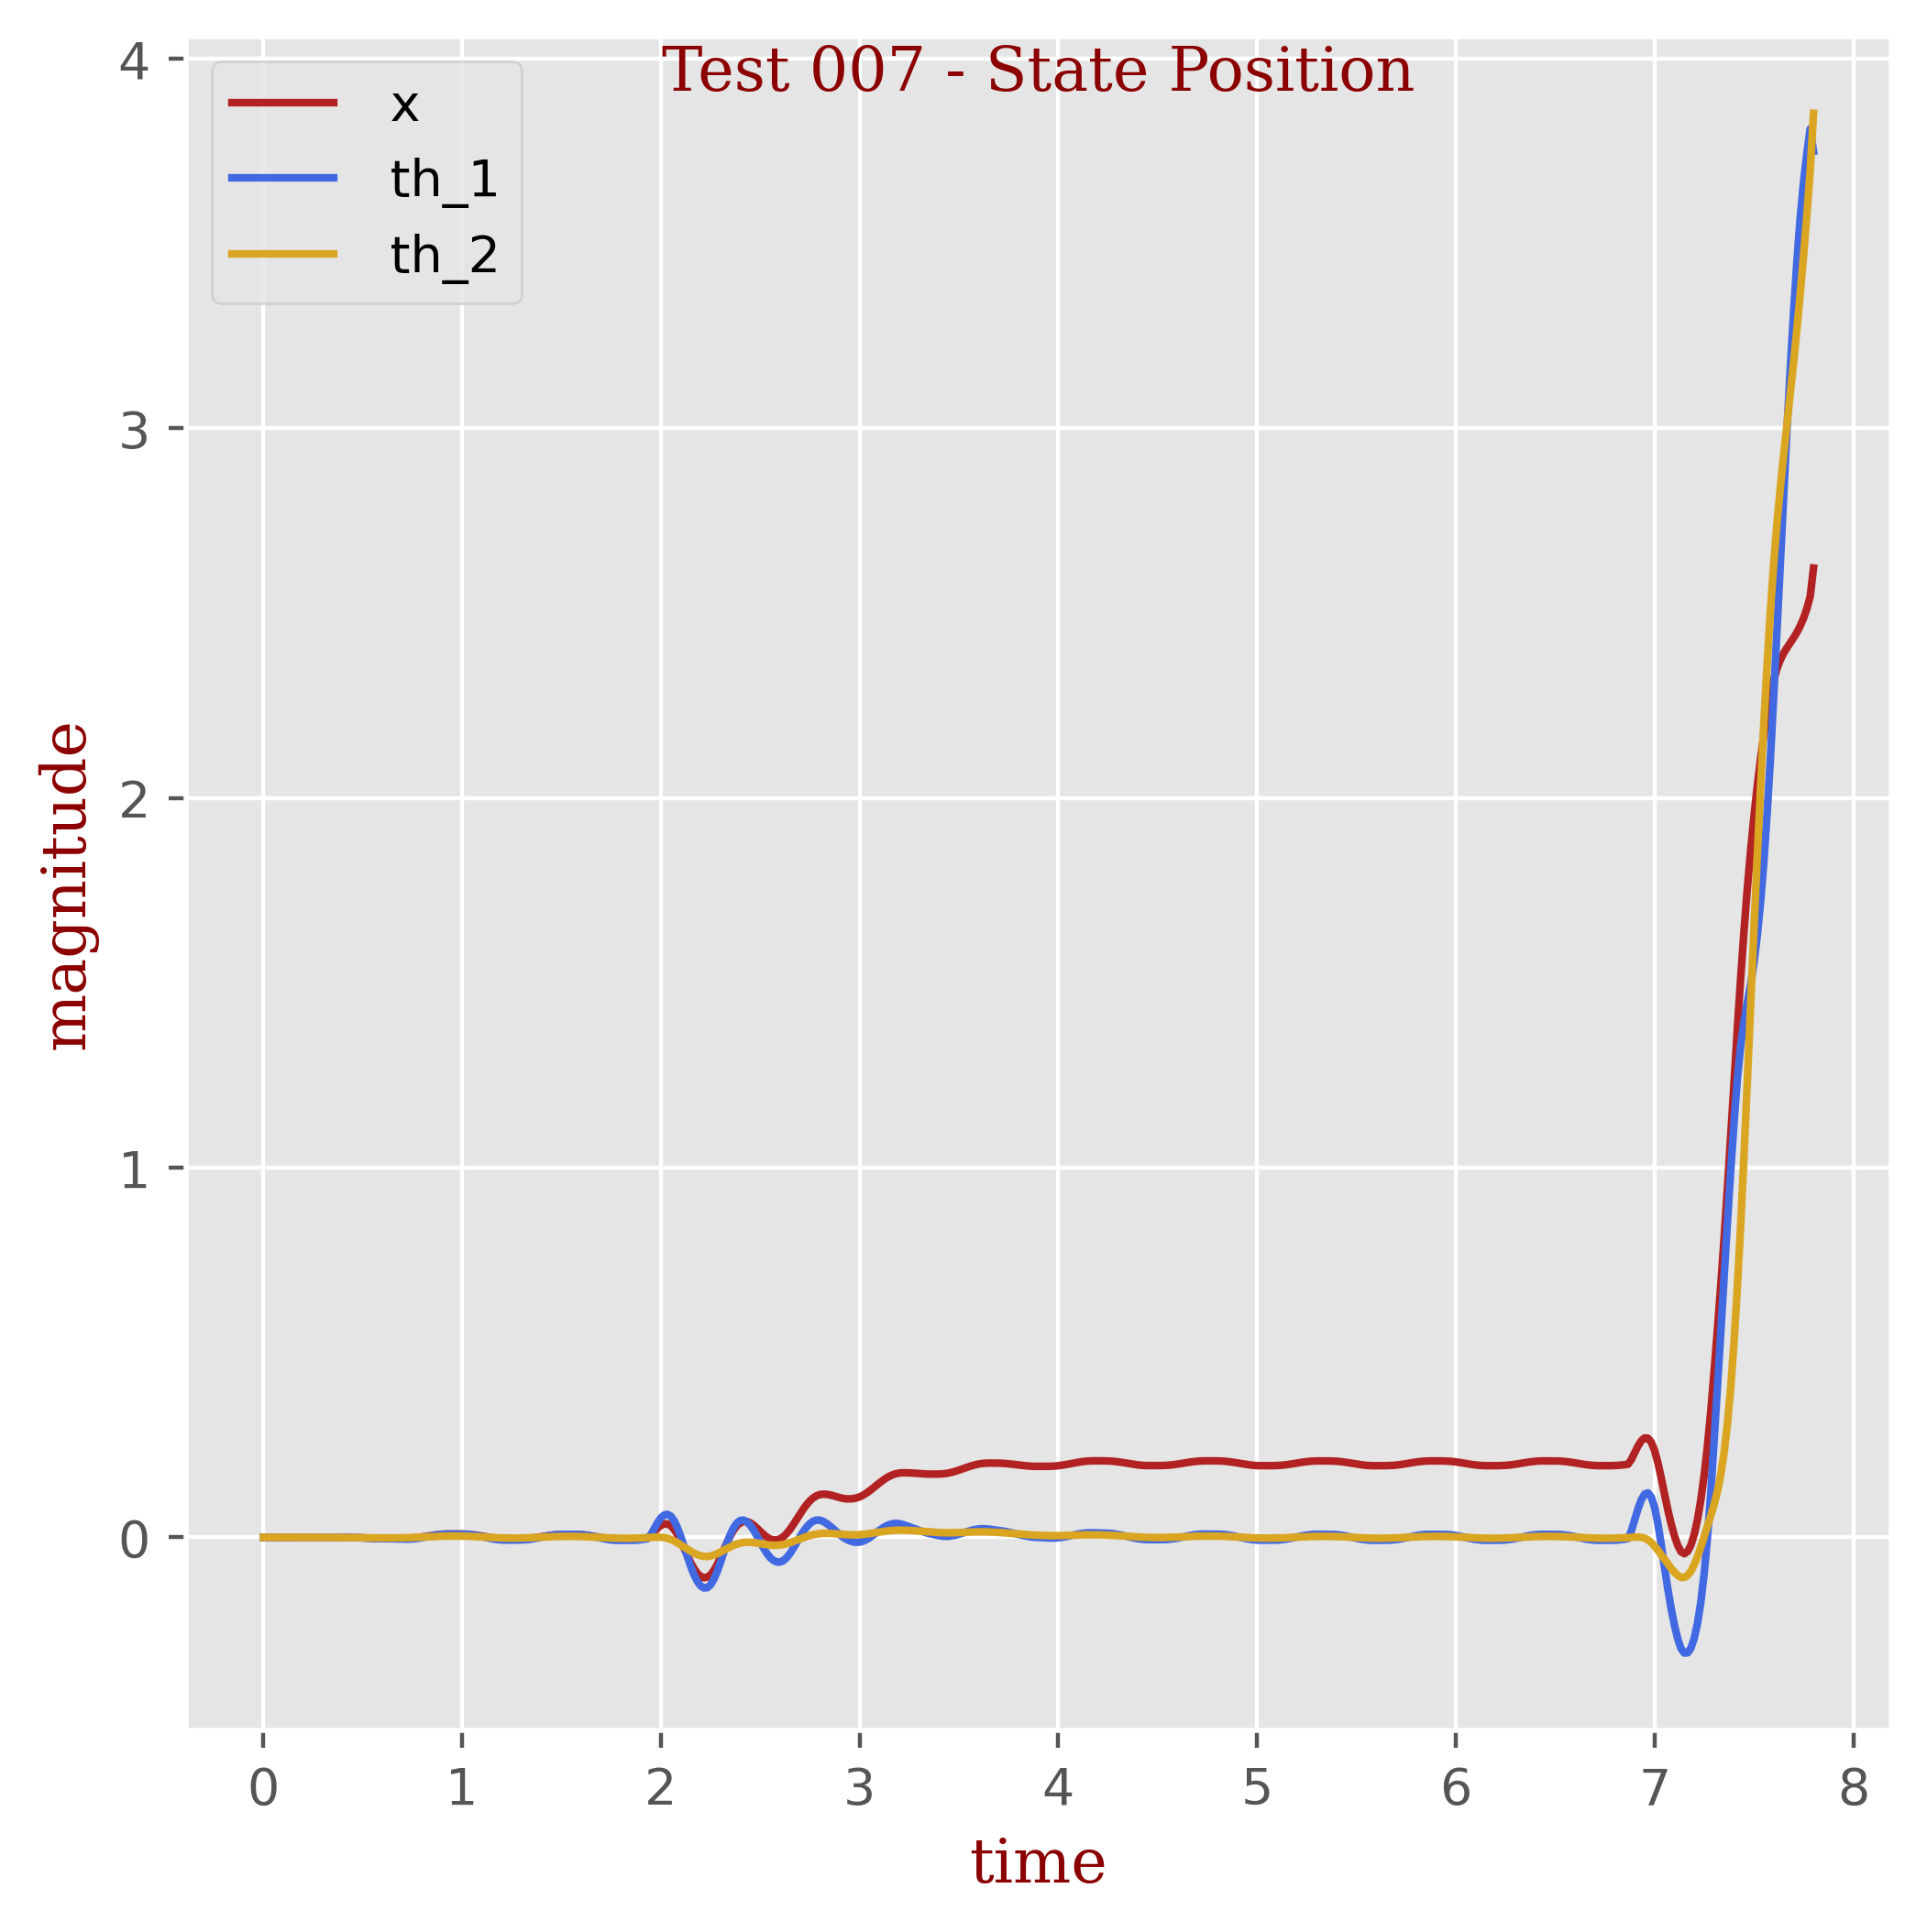
\includegraphics[width=27mm]{Test 007_State_Position.png}}
\subfigure[\(\dot{q}(t)\)]{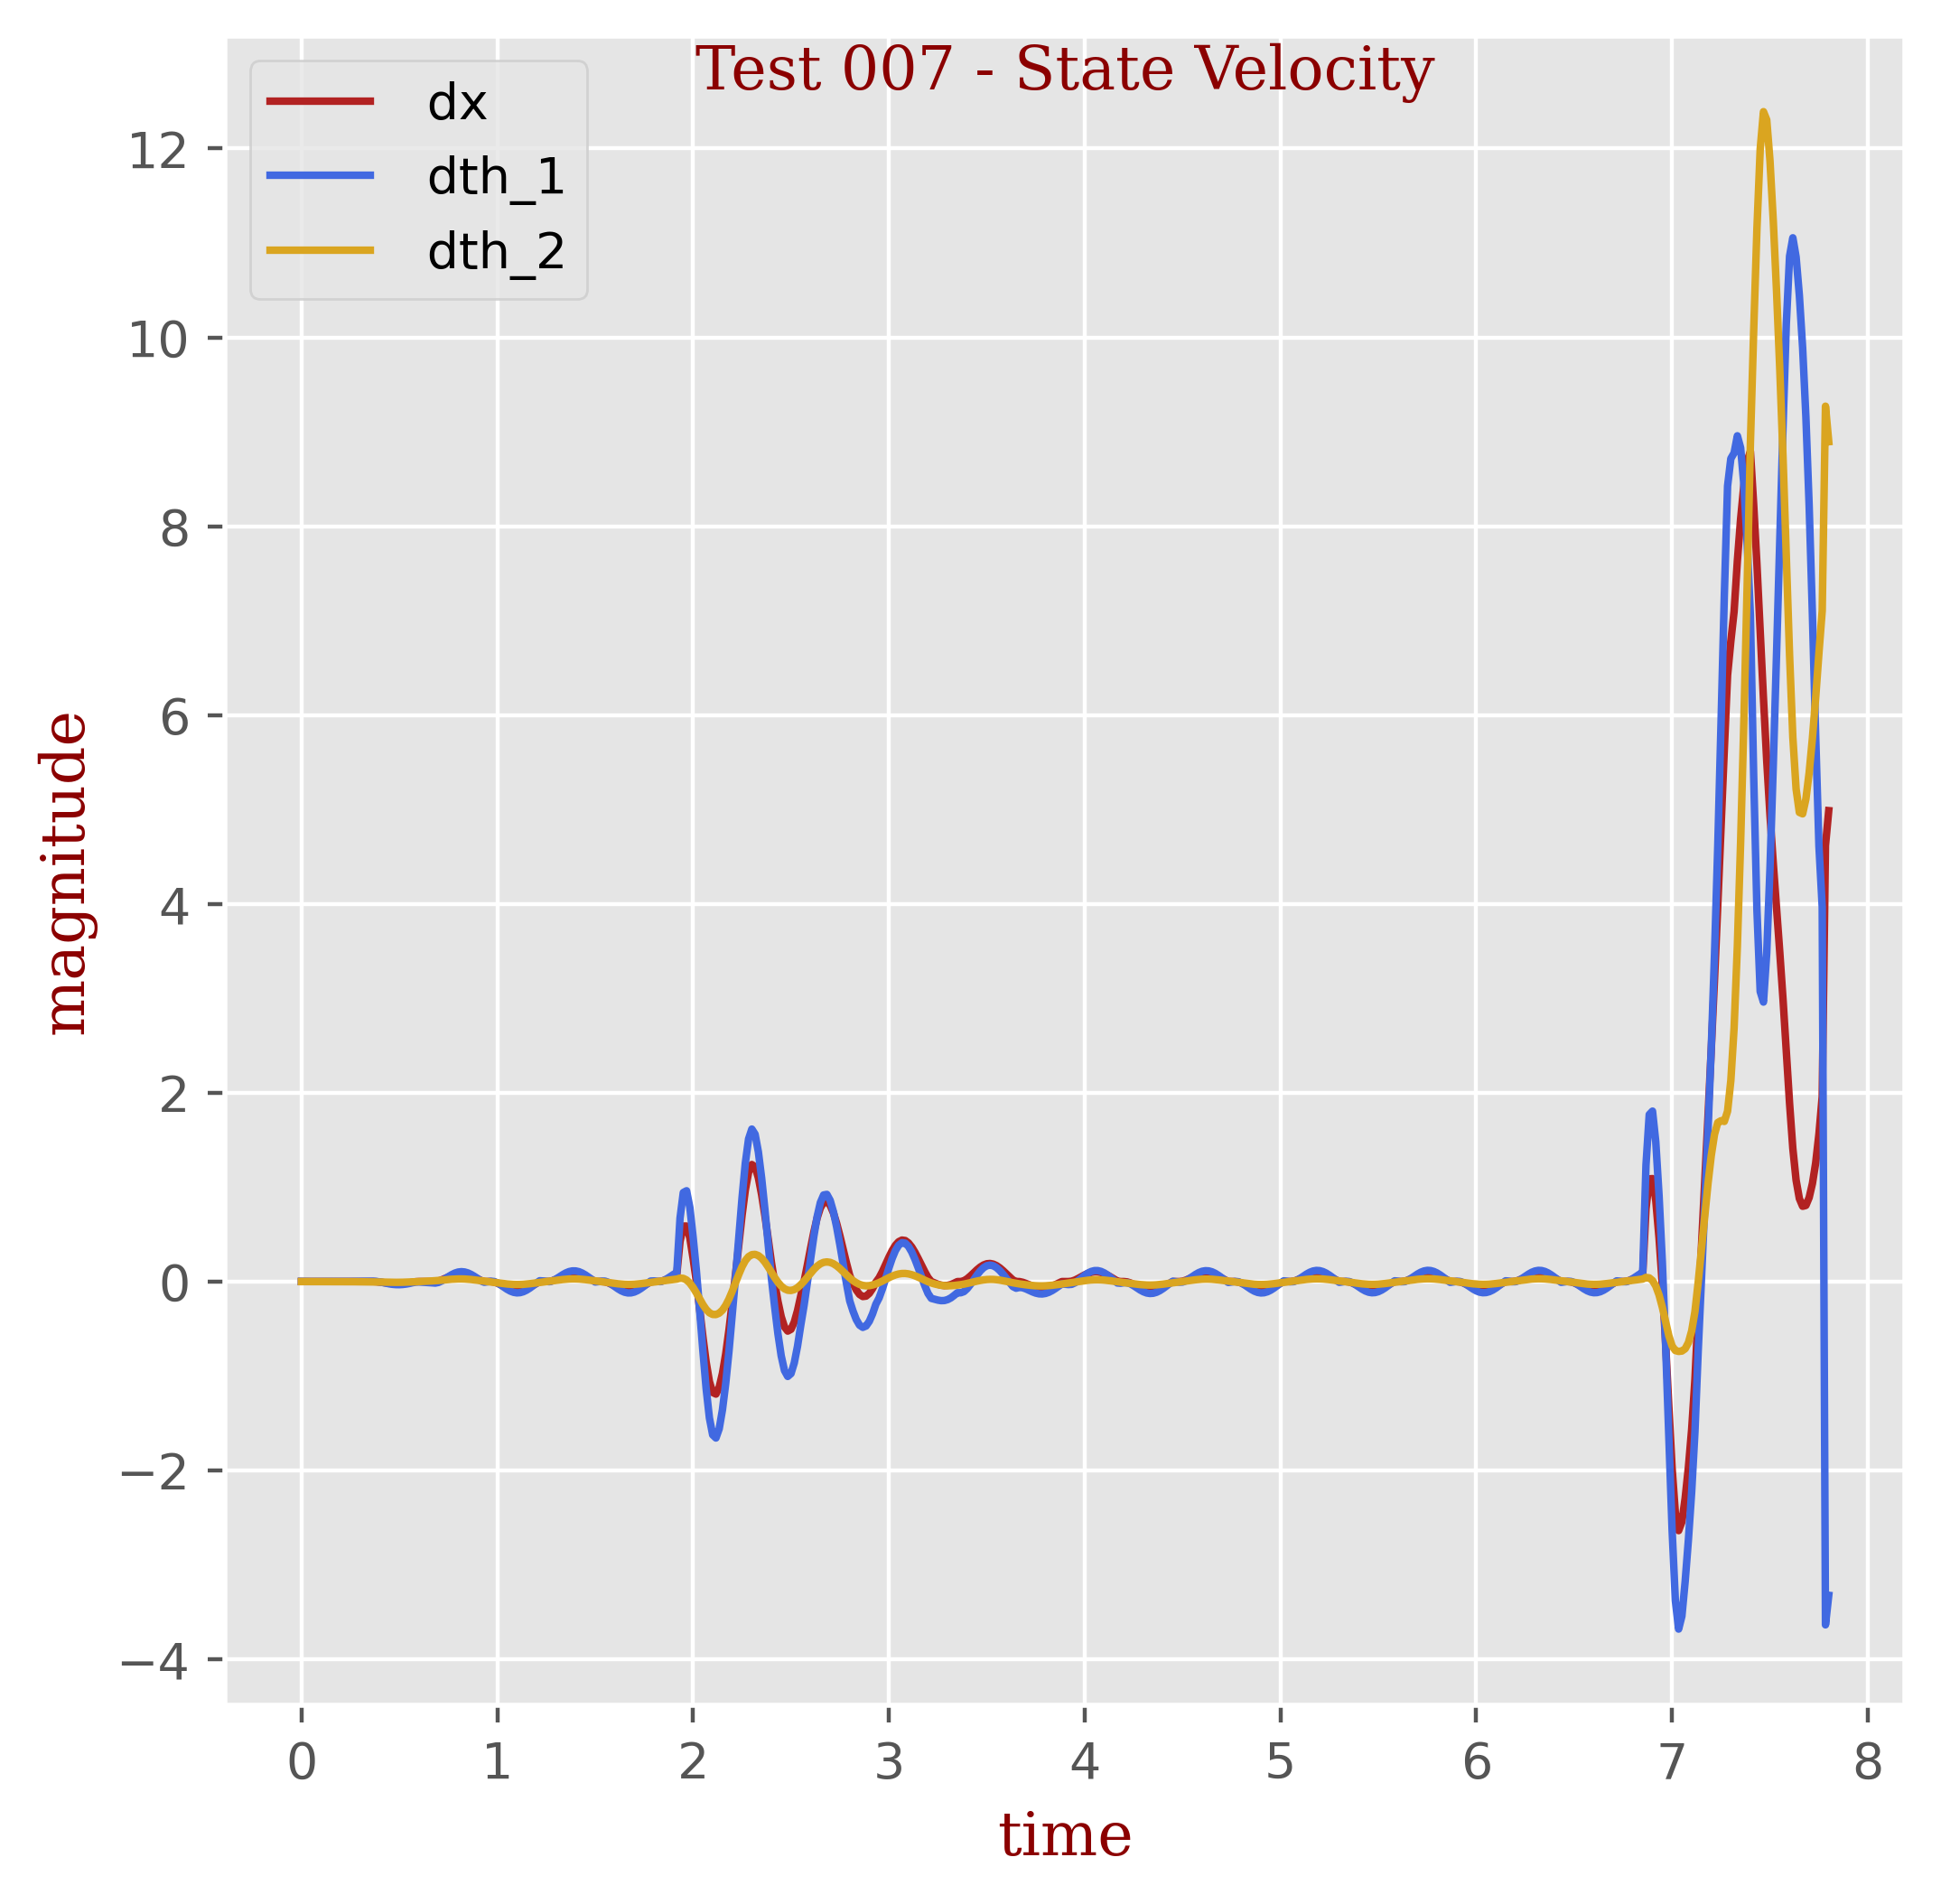
\includegraphics[width=27mm]{Test 007_State_Velocity.png}}
\subfigure[\(J(t)\)]{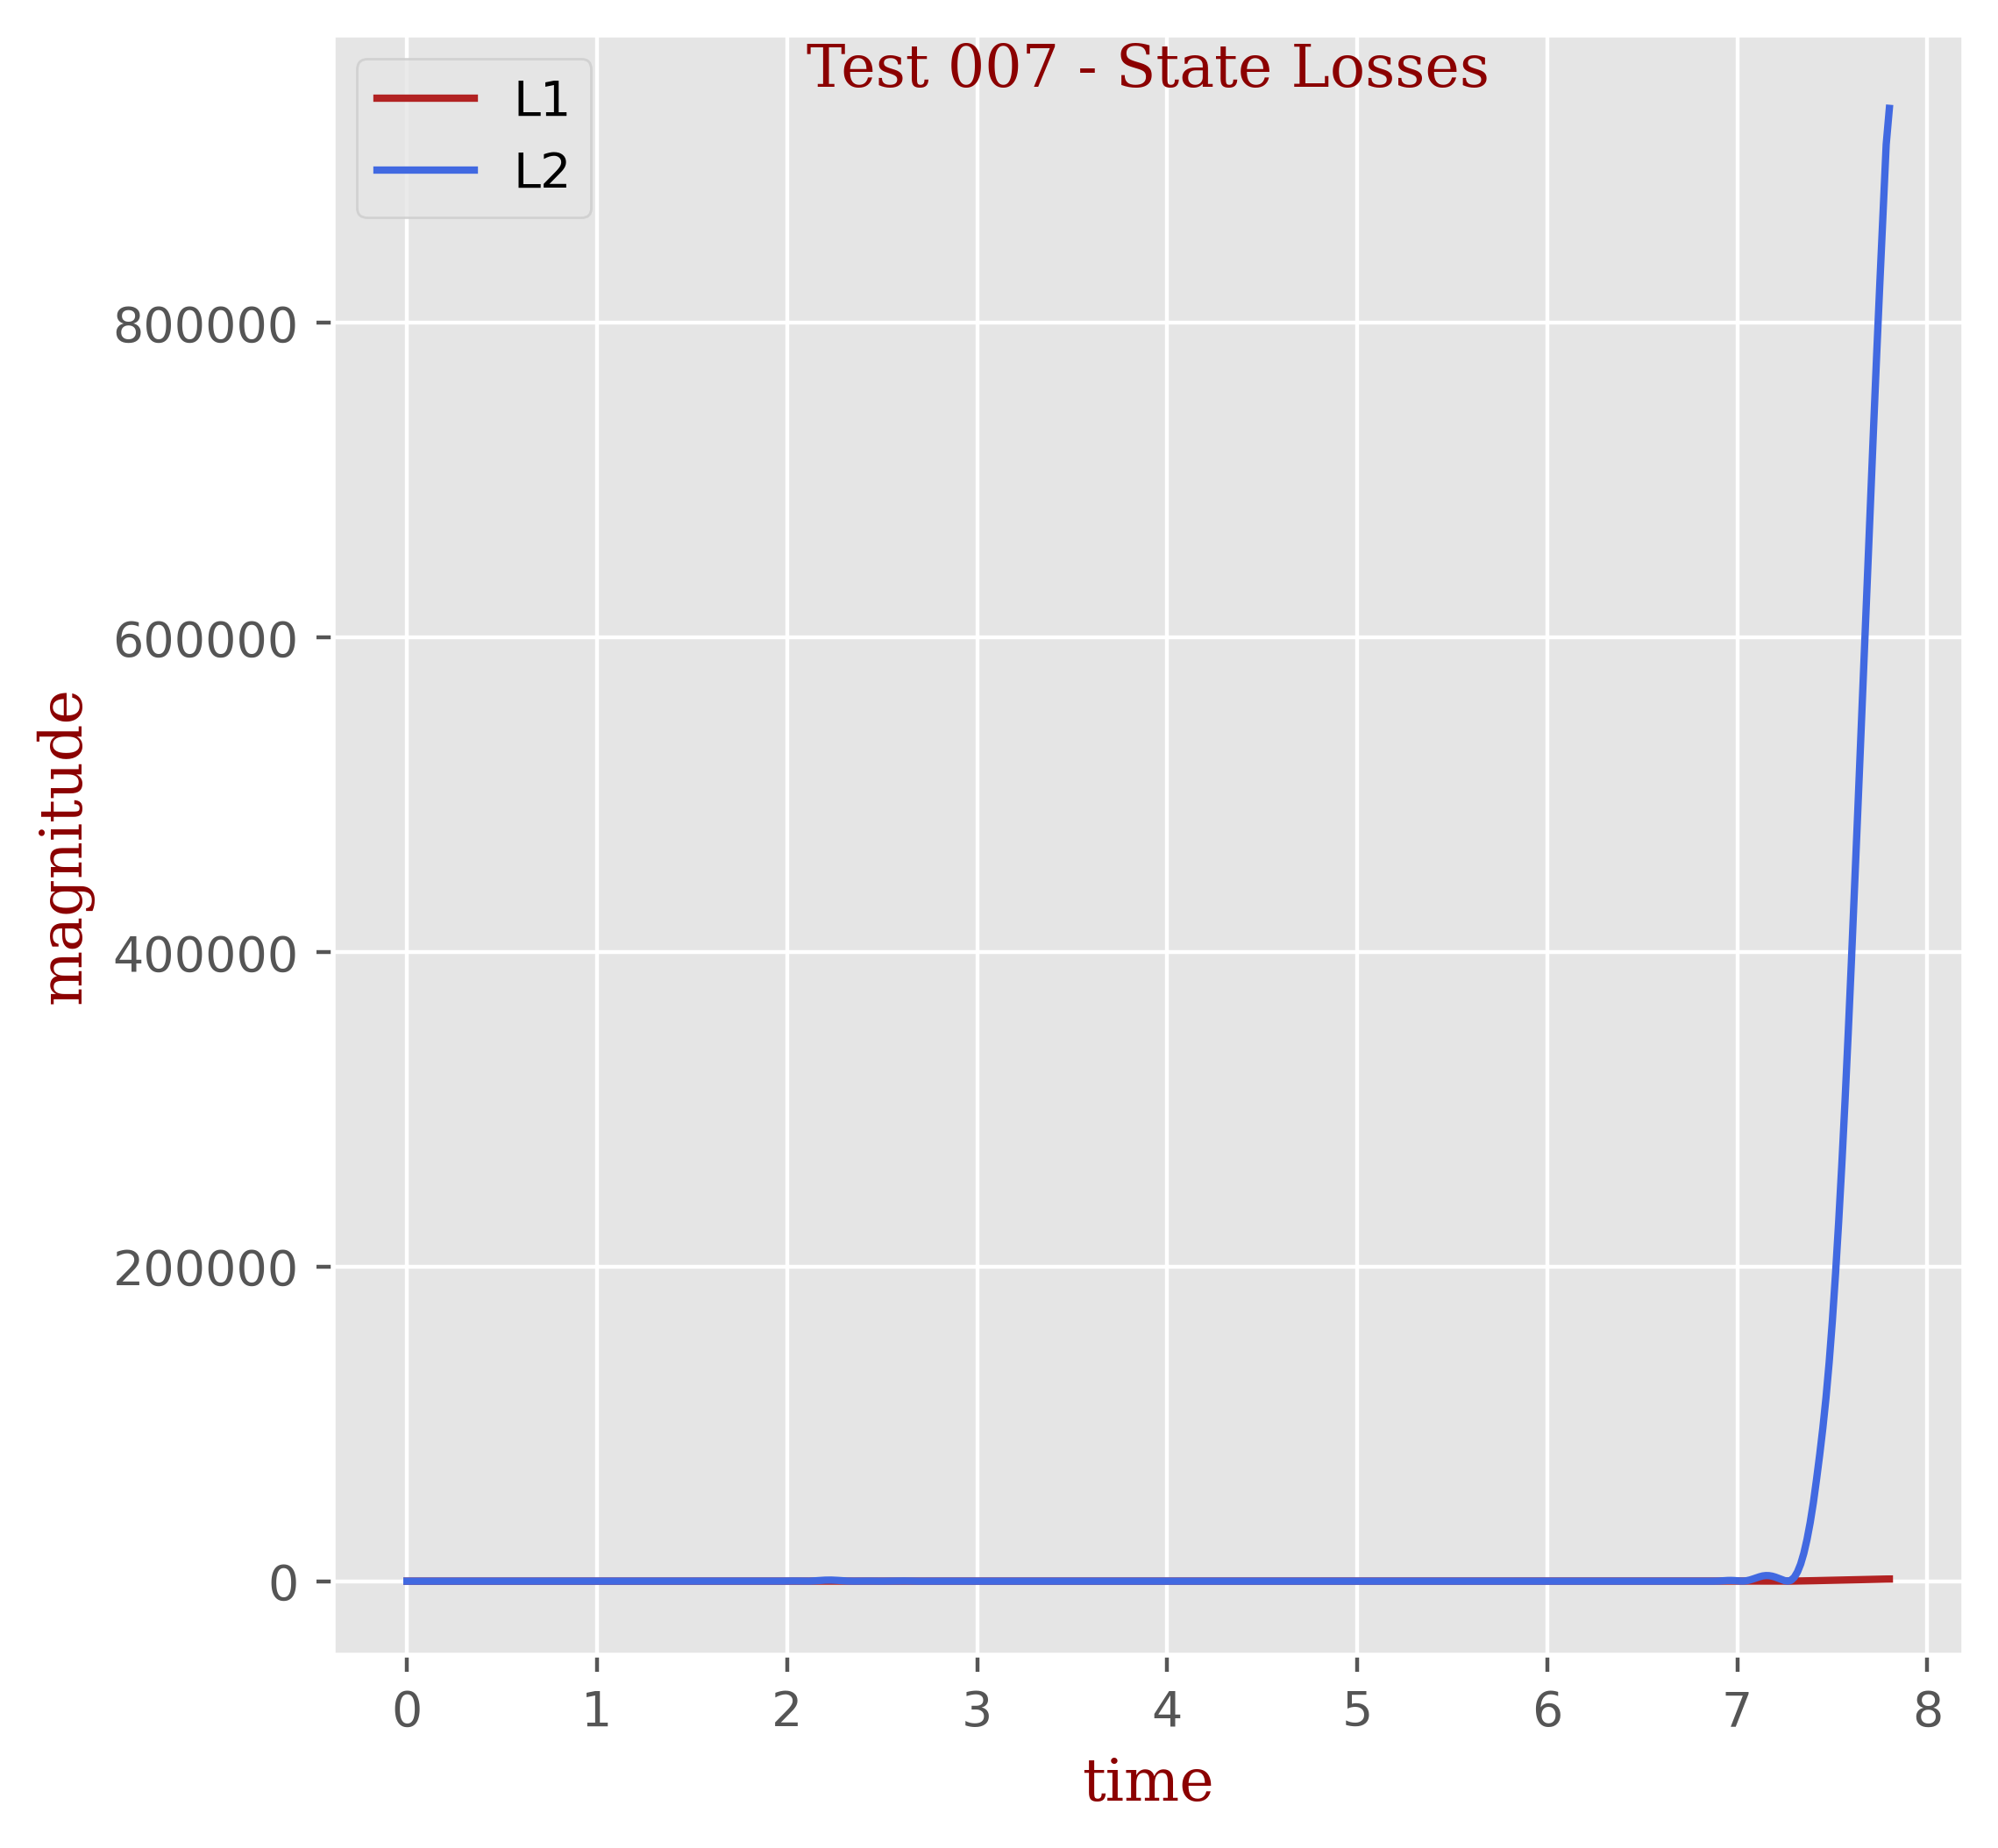
\includegraphics[width=27mm]{Test 007_State_Losses.png}}
\caption{Test 007}
\label{fig:t007}
\end{figure}


\begin{figure}
\centering
\subfigure[\(q(t)\)]{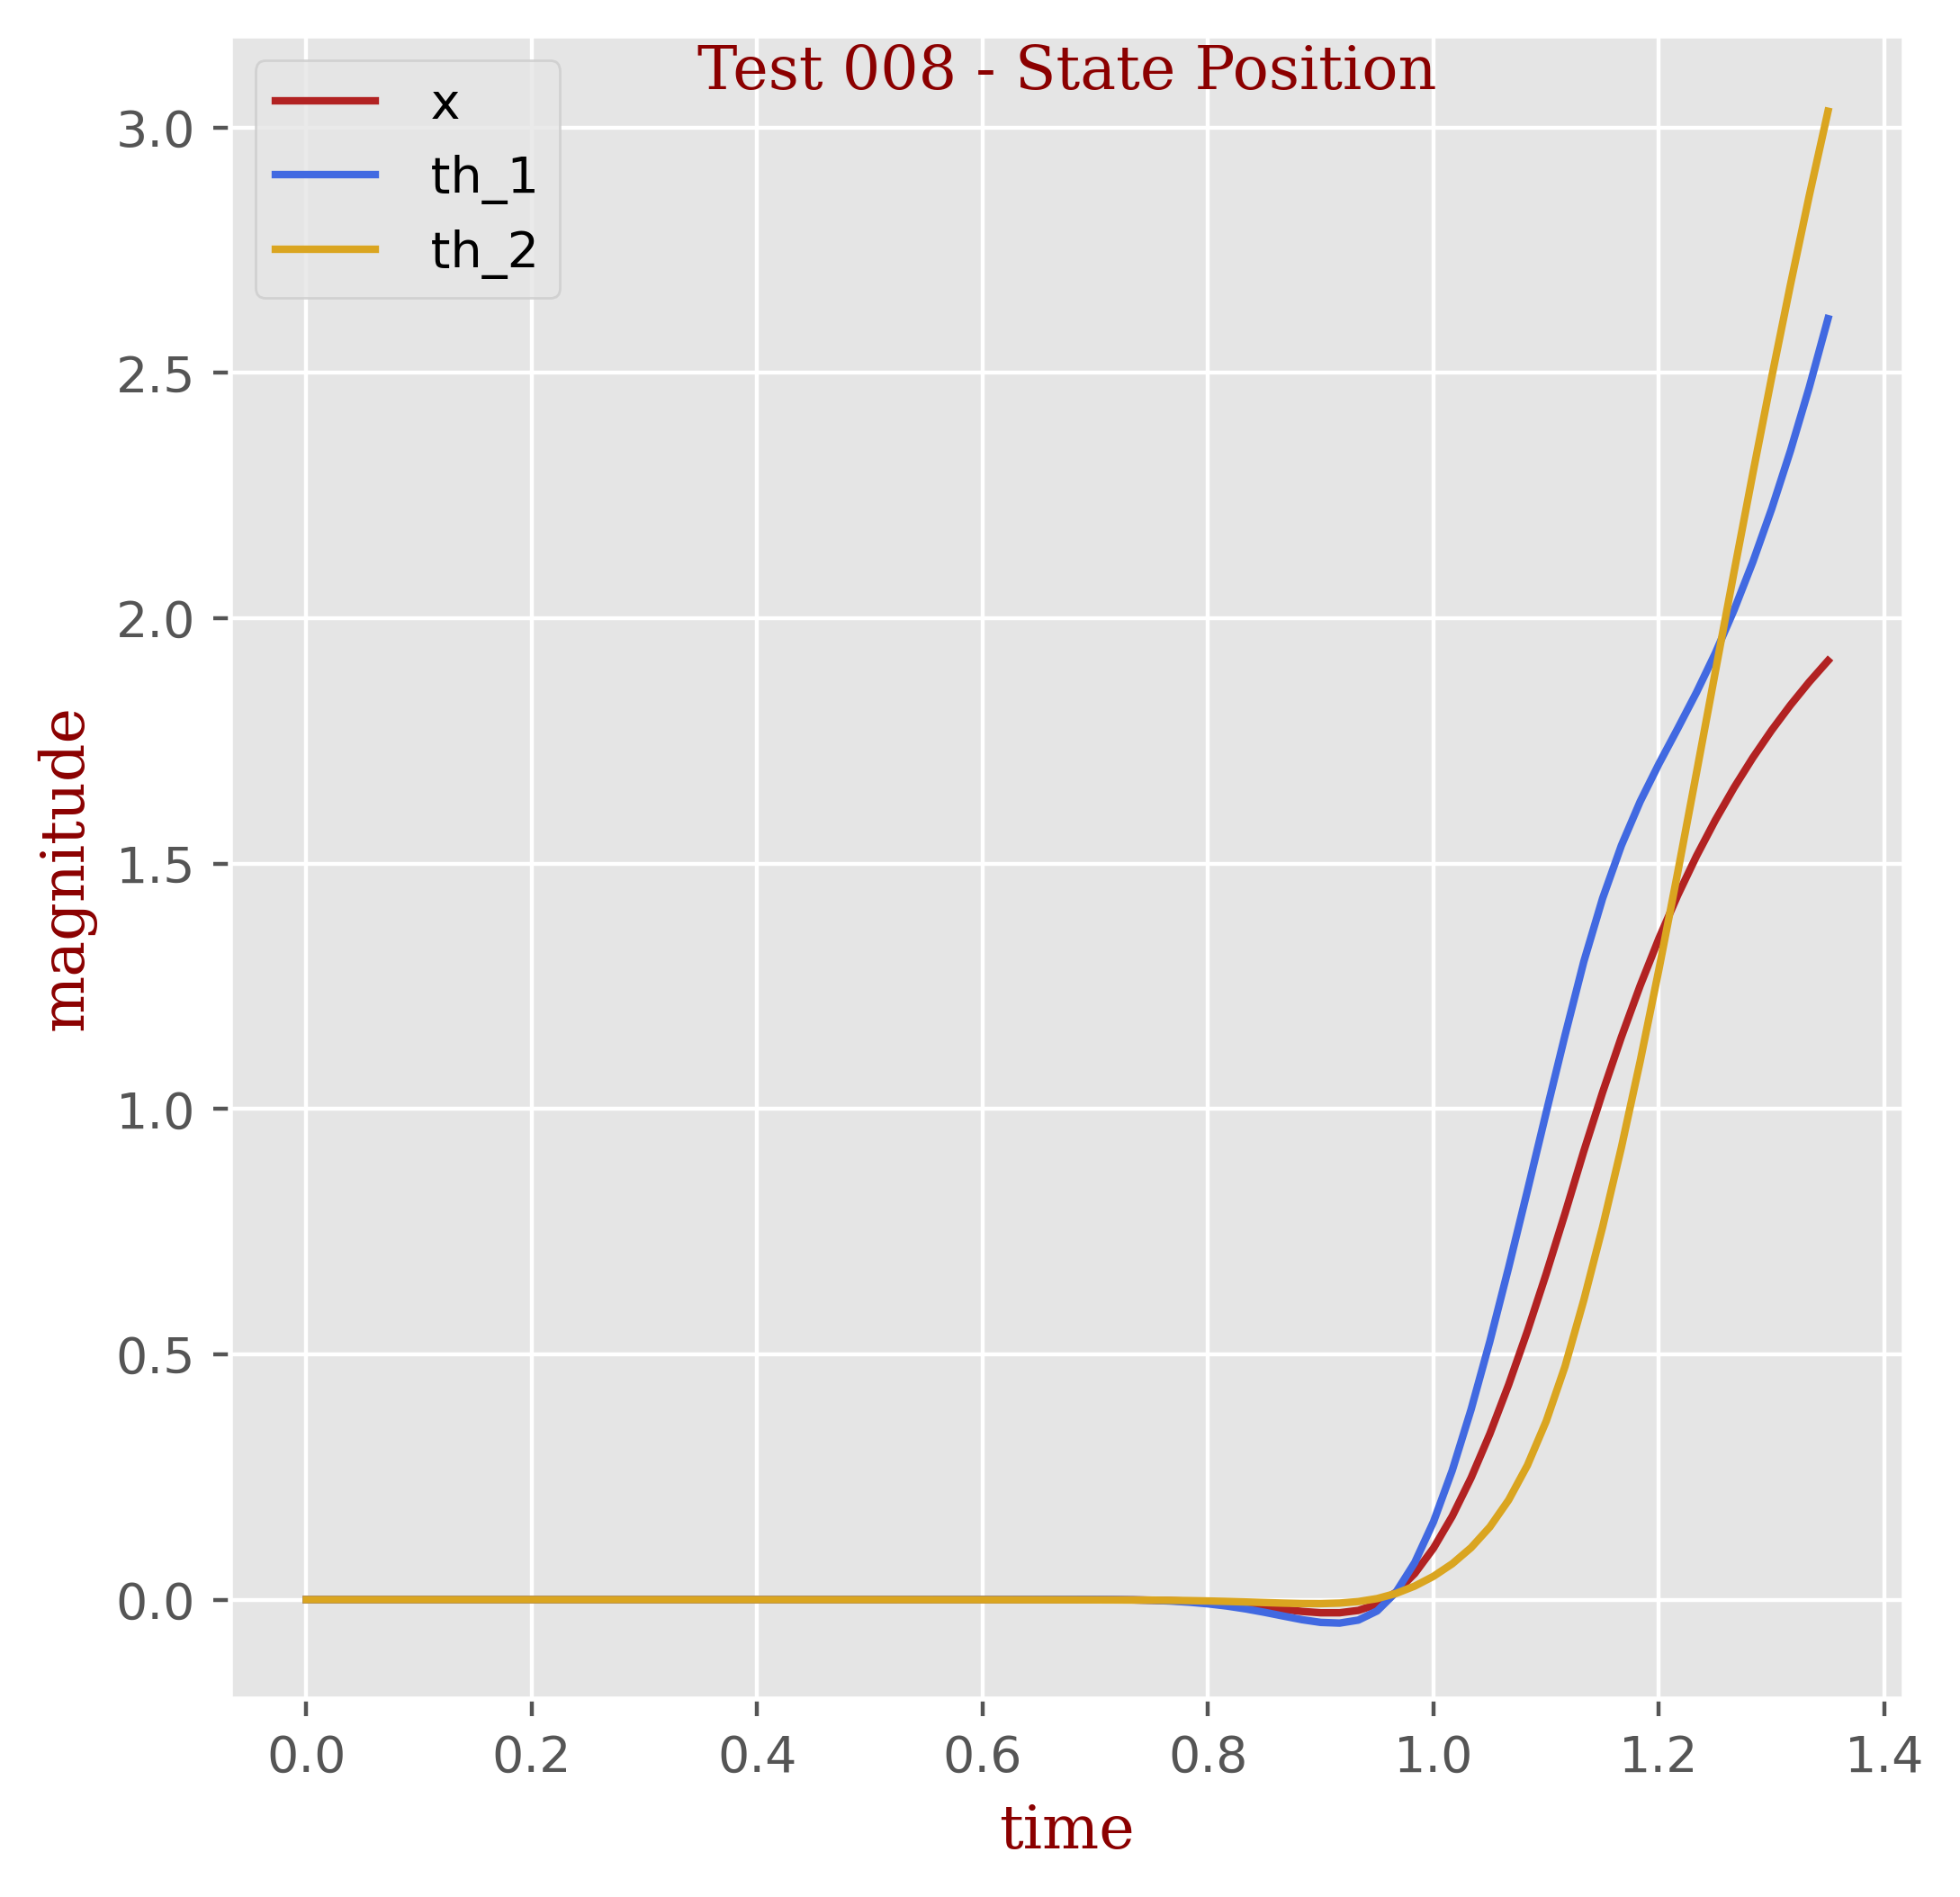
\includegraphics[width=27mm]{Test 008_State_Position.png}}
\subfigure[\(\dot{q}(t)\)]{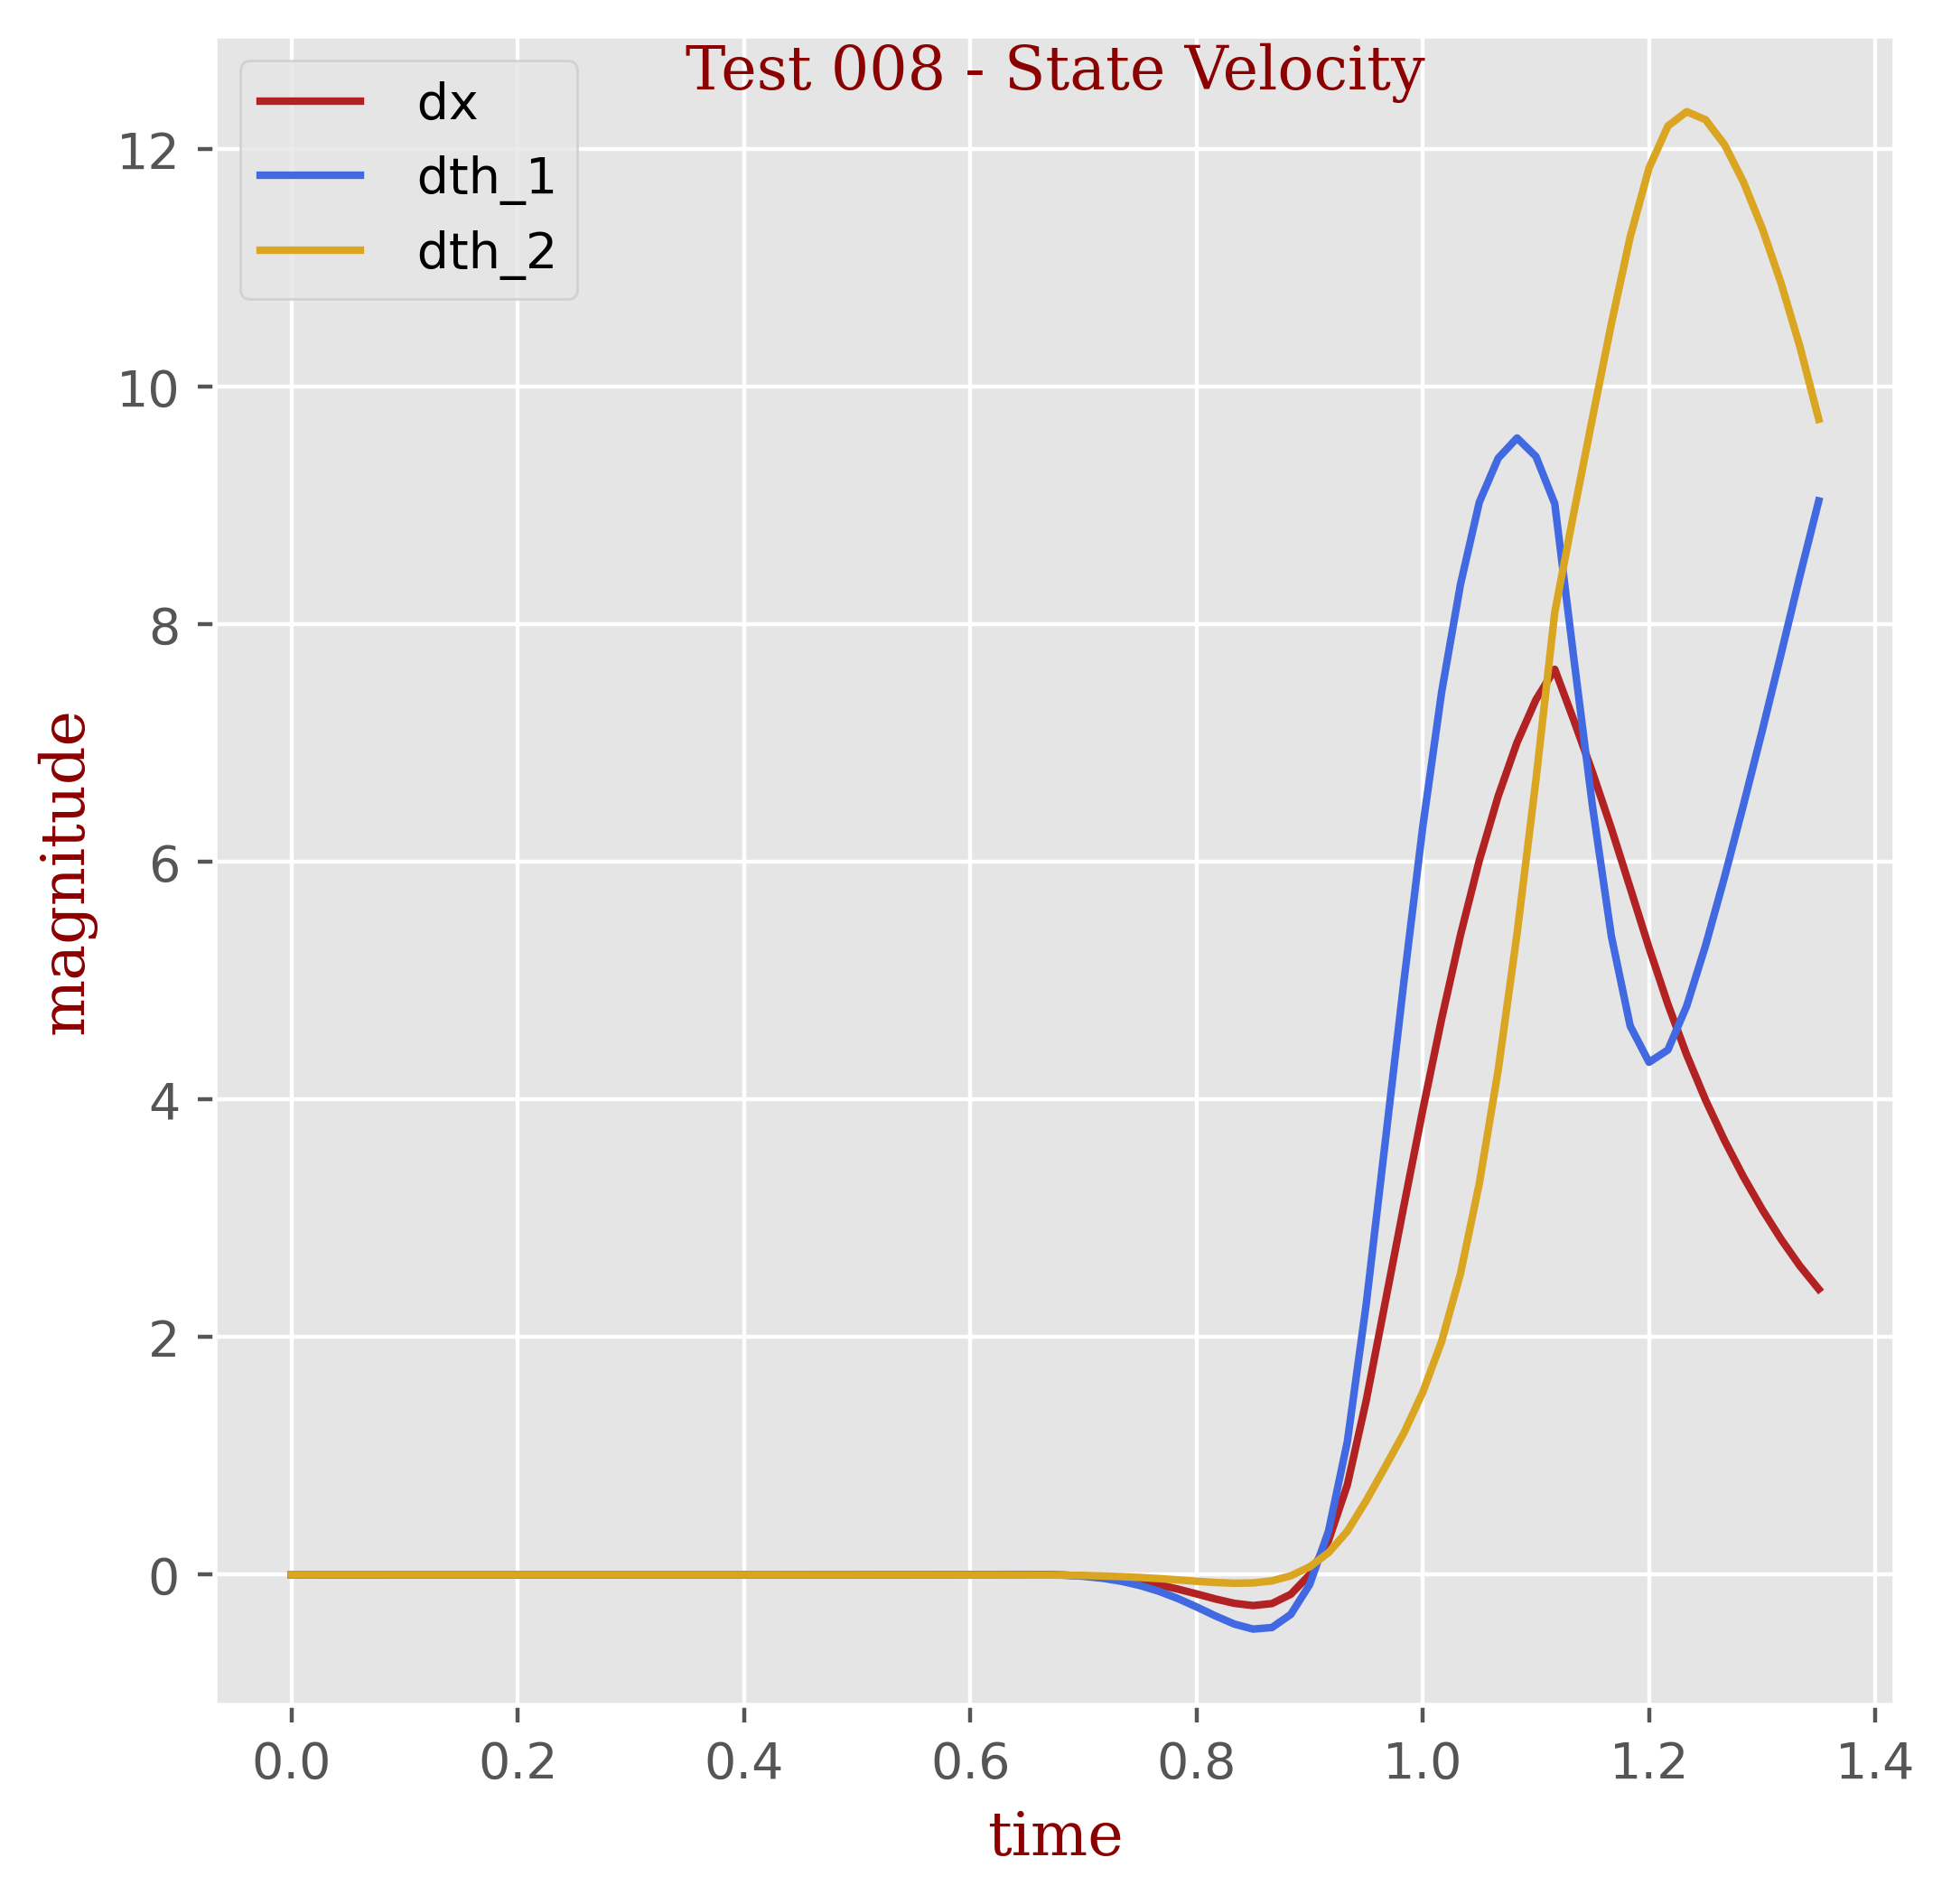
\includegraphics[width=27mm]{Test 008_State_Velocity.png}}
\subfigure[\(J(t)\)]{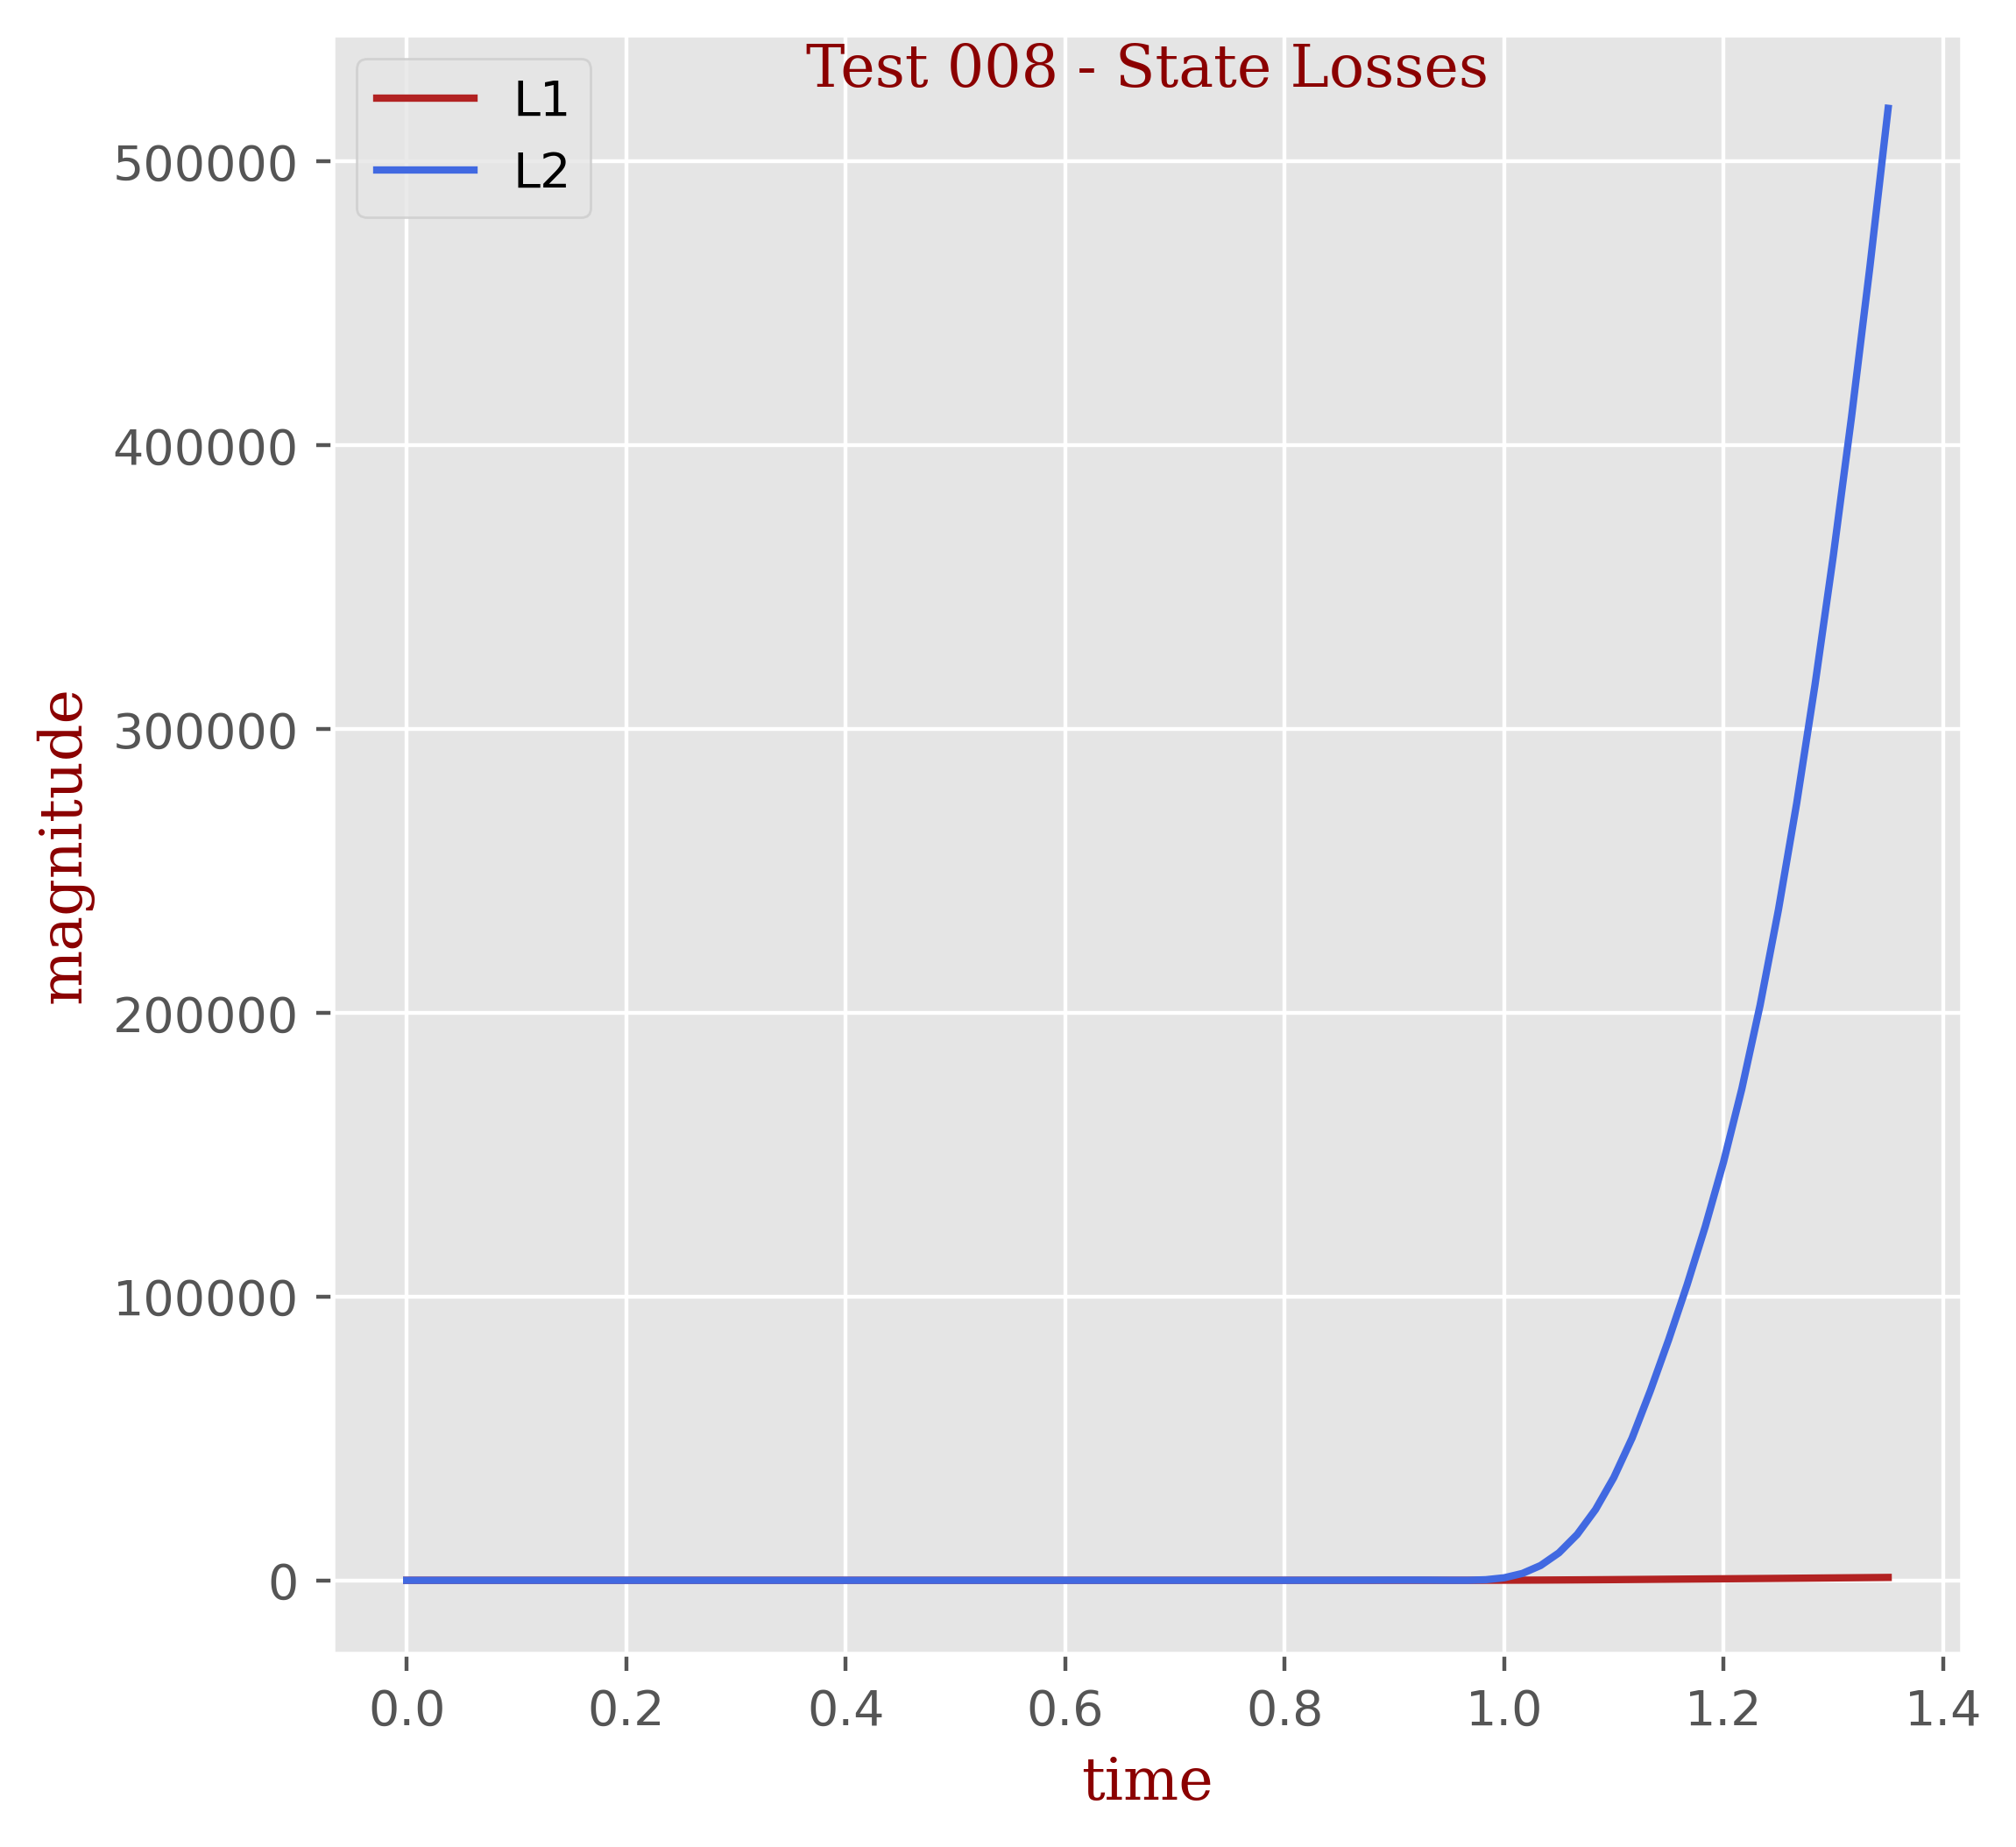
\includegraphics[width=27mm]{Test 008_State_Losses.png}}
\caption{Test 008}
\label{fig:t008}
\end{figure}

\begin{figure}
\centering
\subfigure[\(q(t)\)]{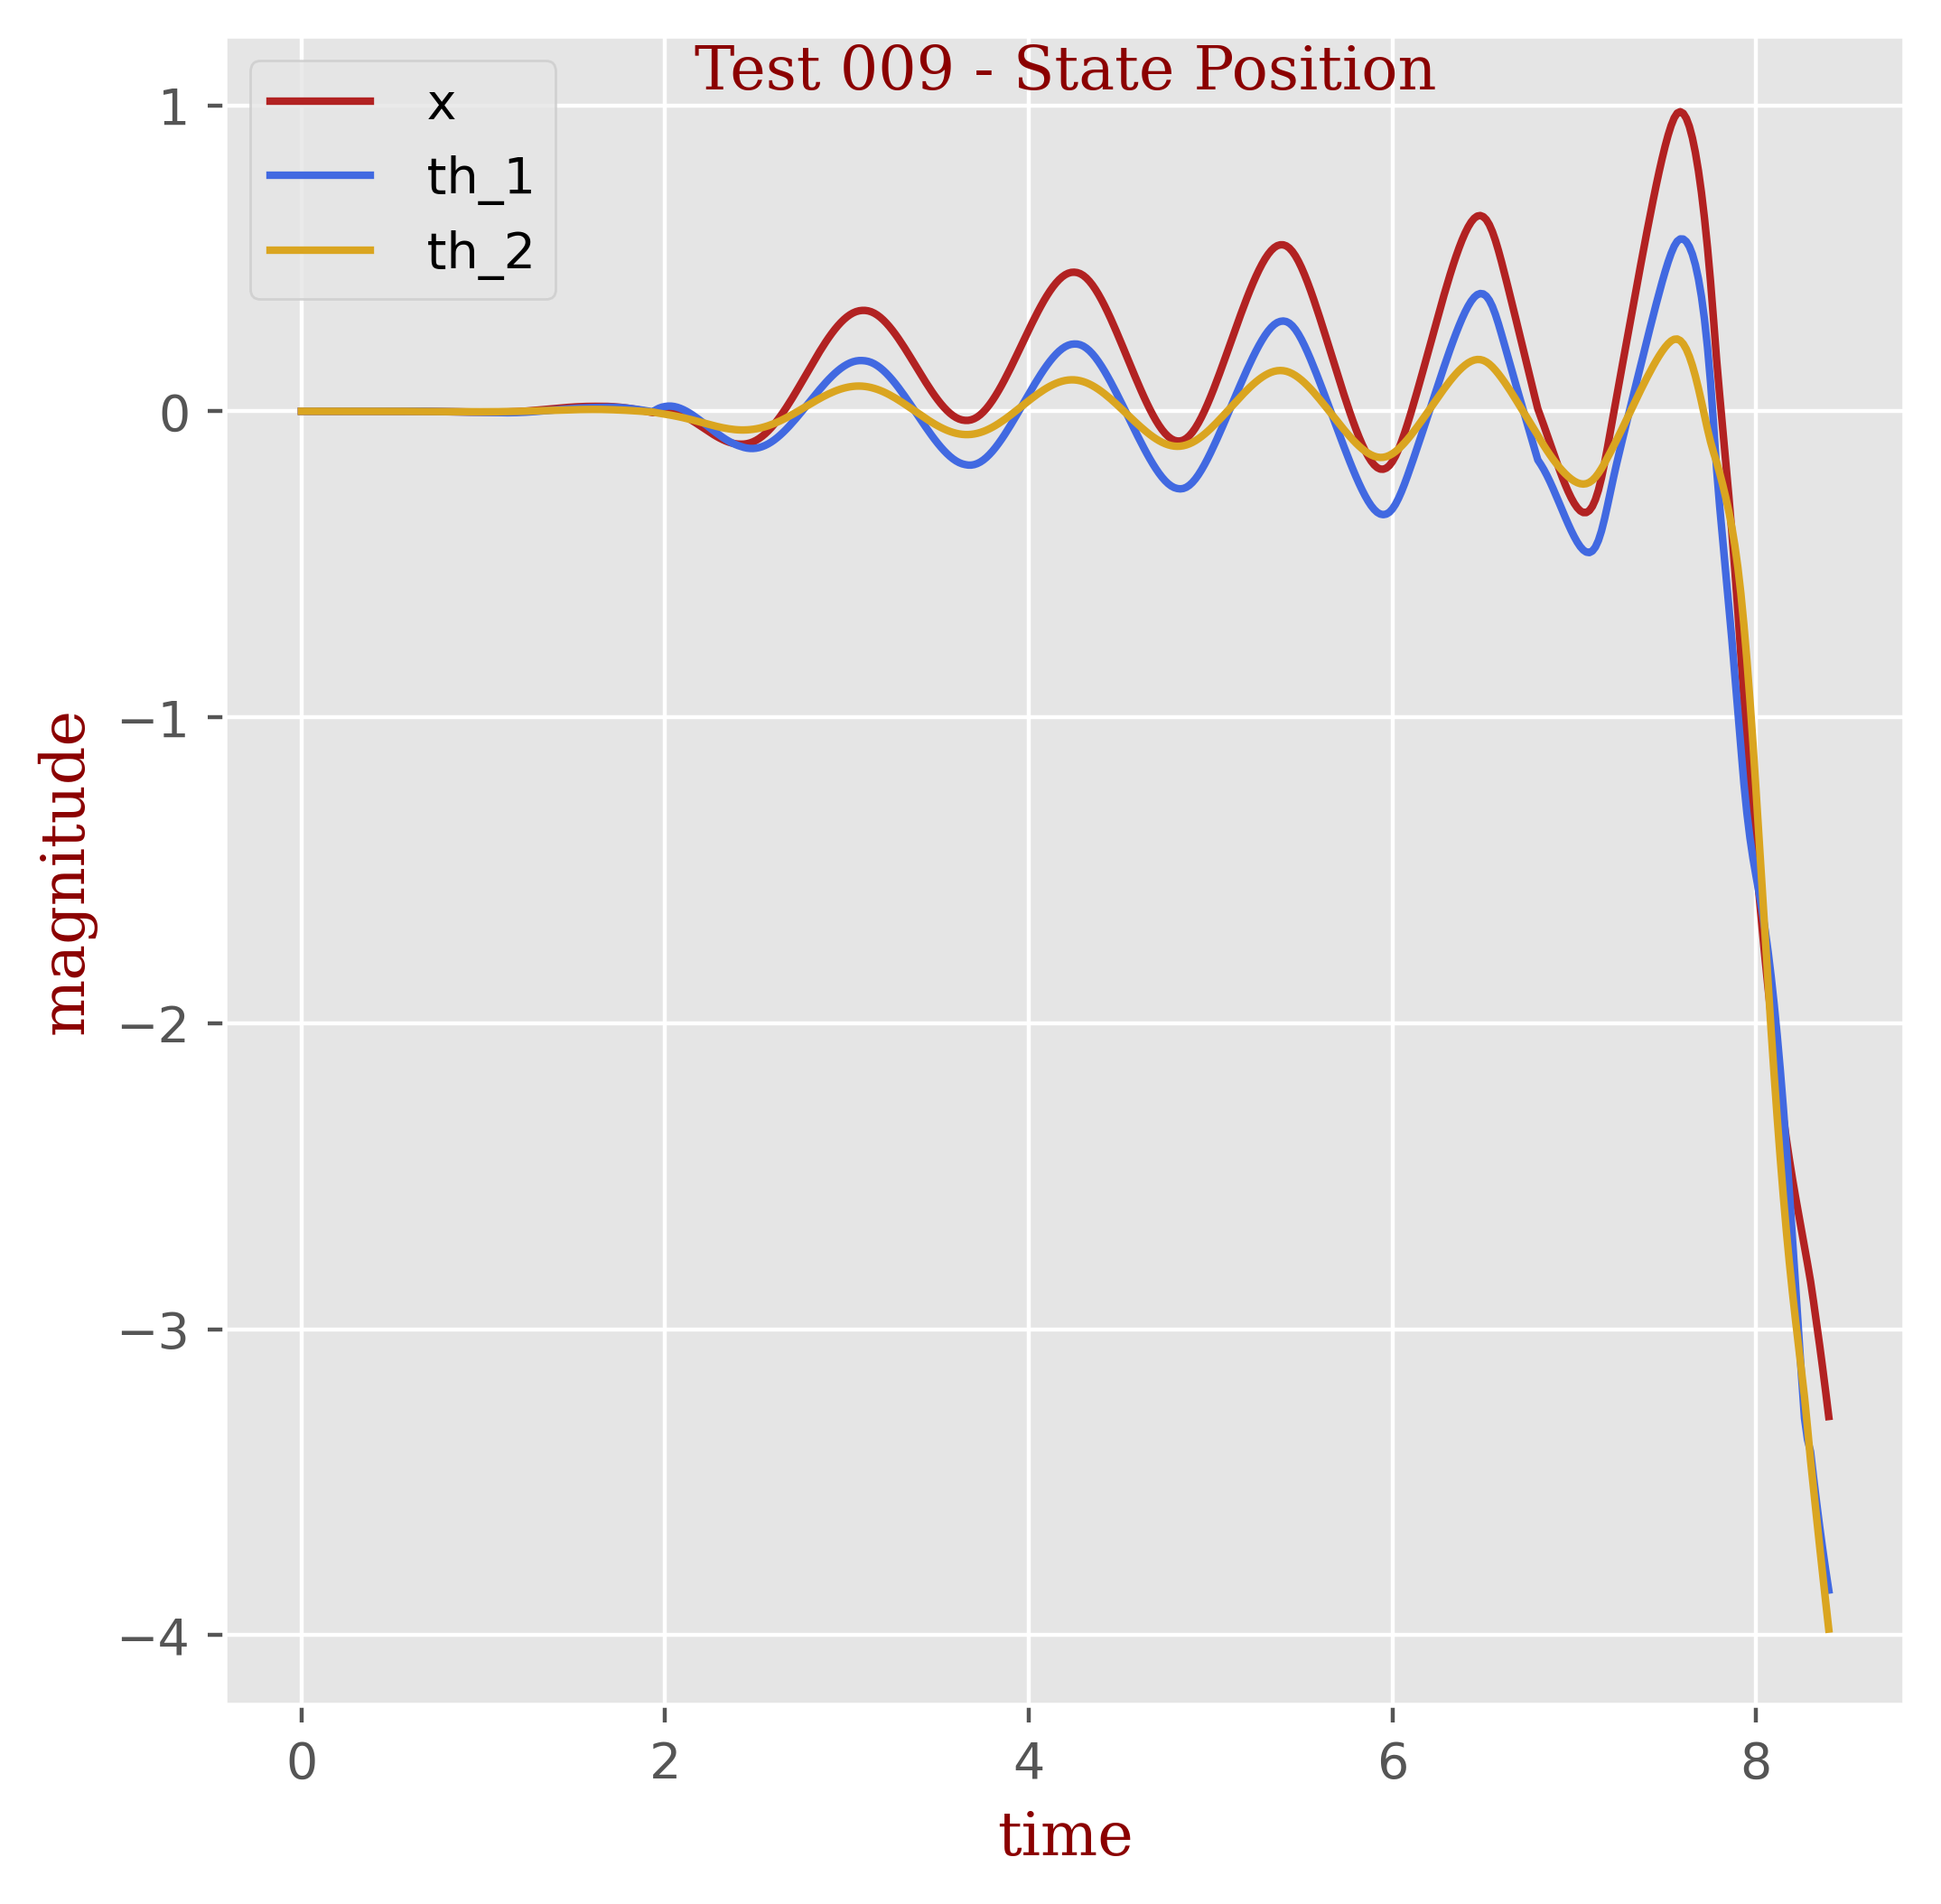
\includegraphics[width=27mm]{Test 009_State_Position.png}}
\subfigure[\(\dot{q}(t)\)]{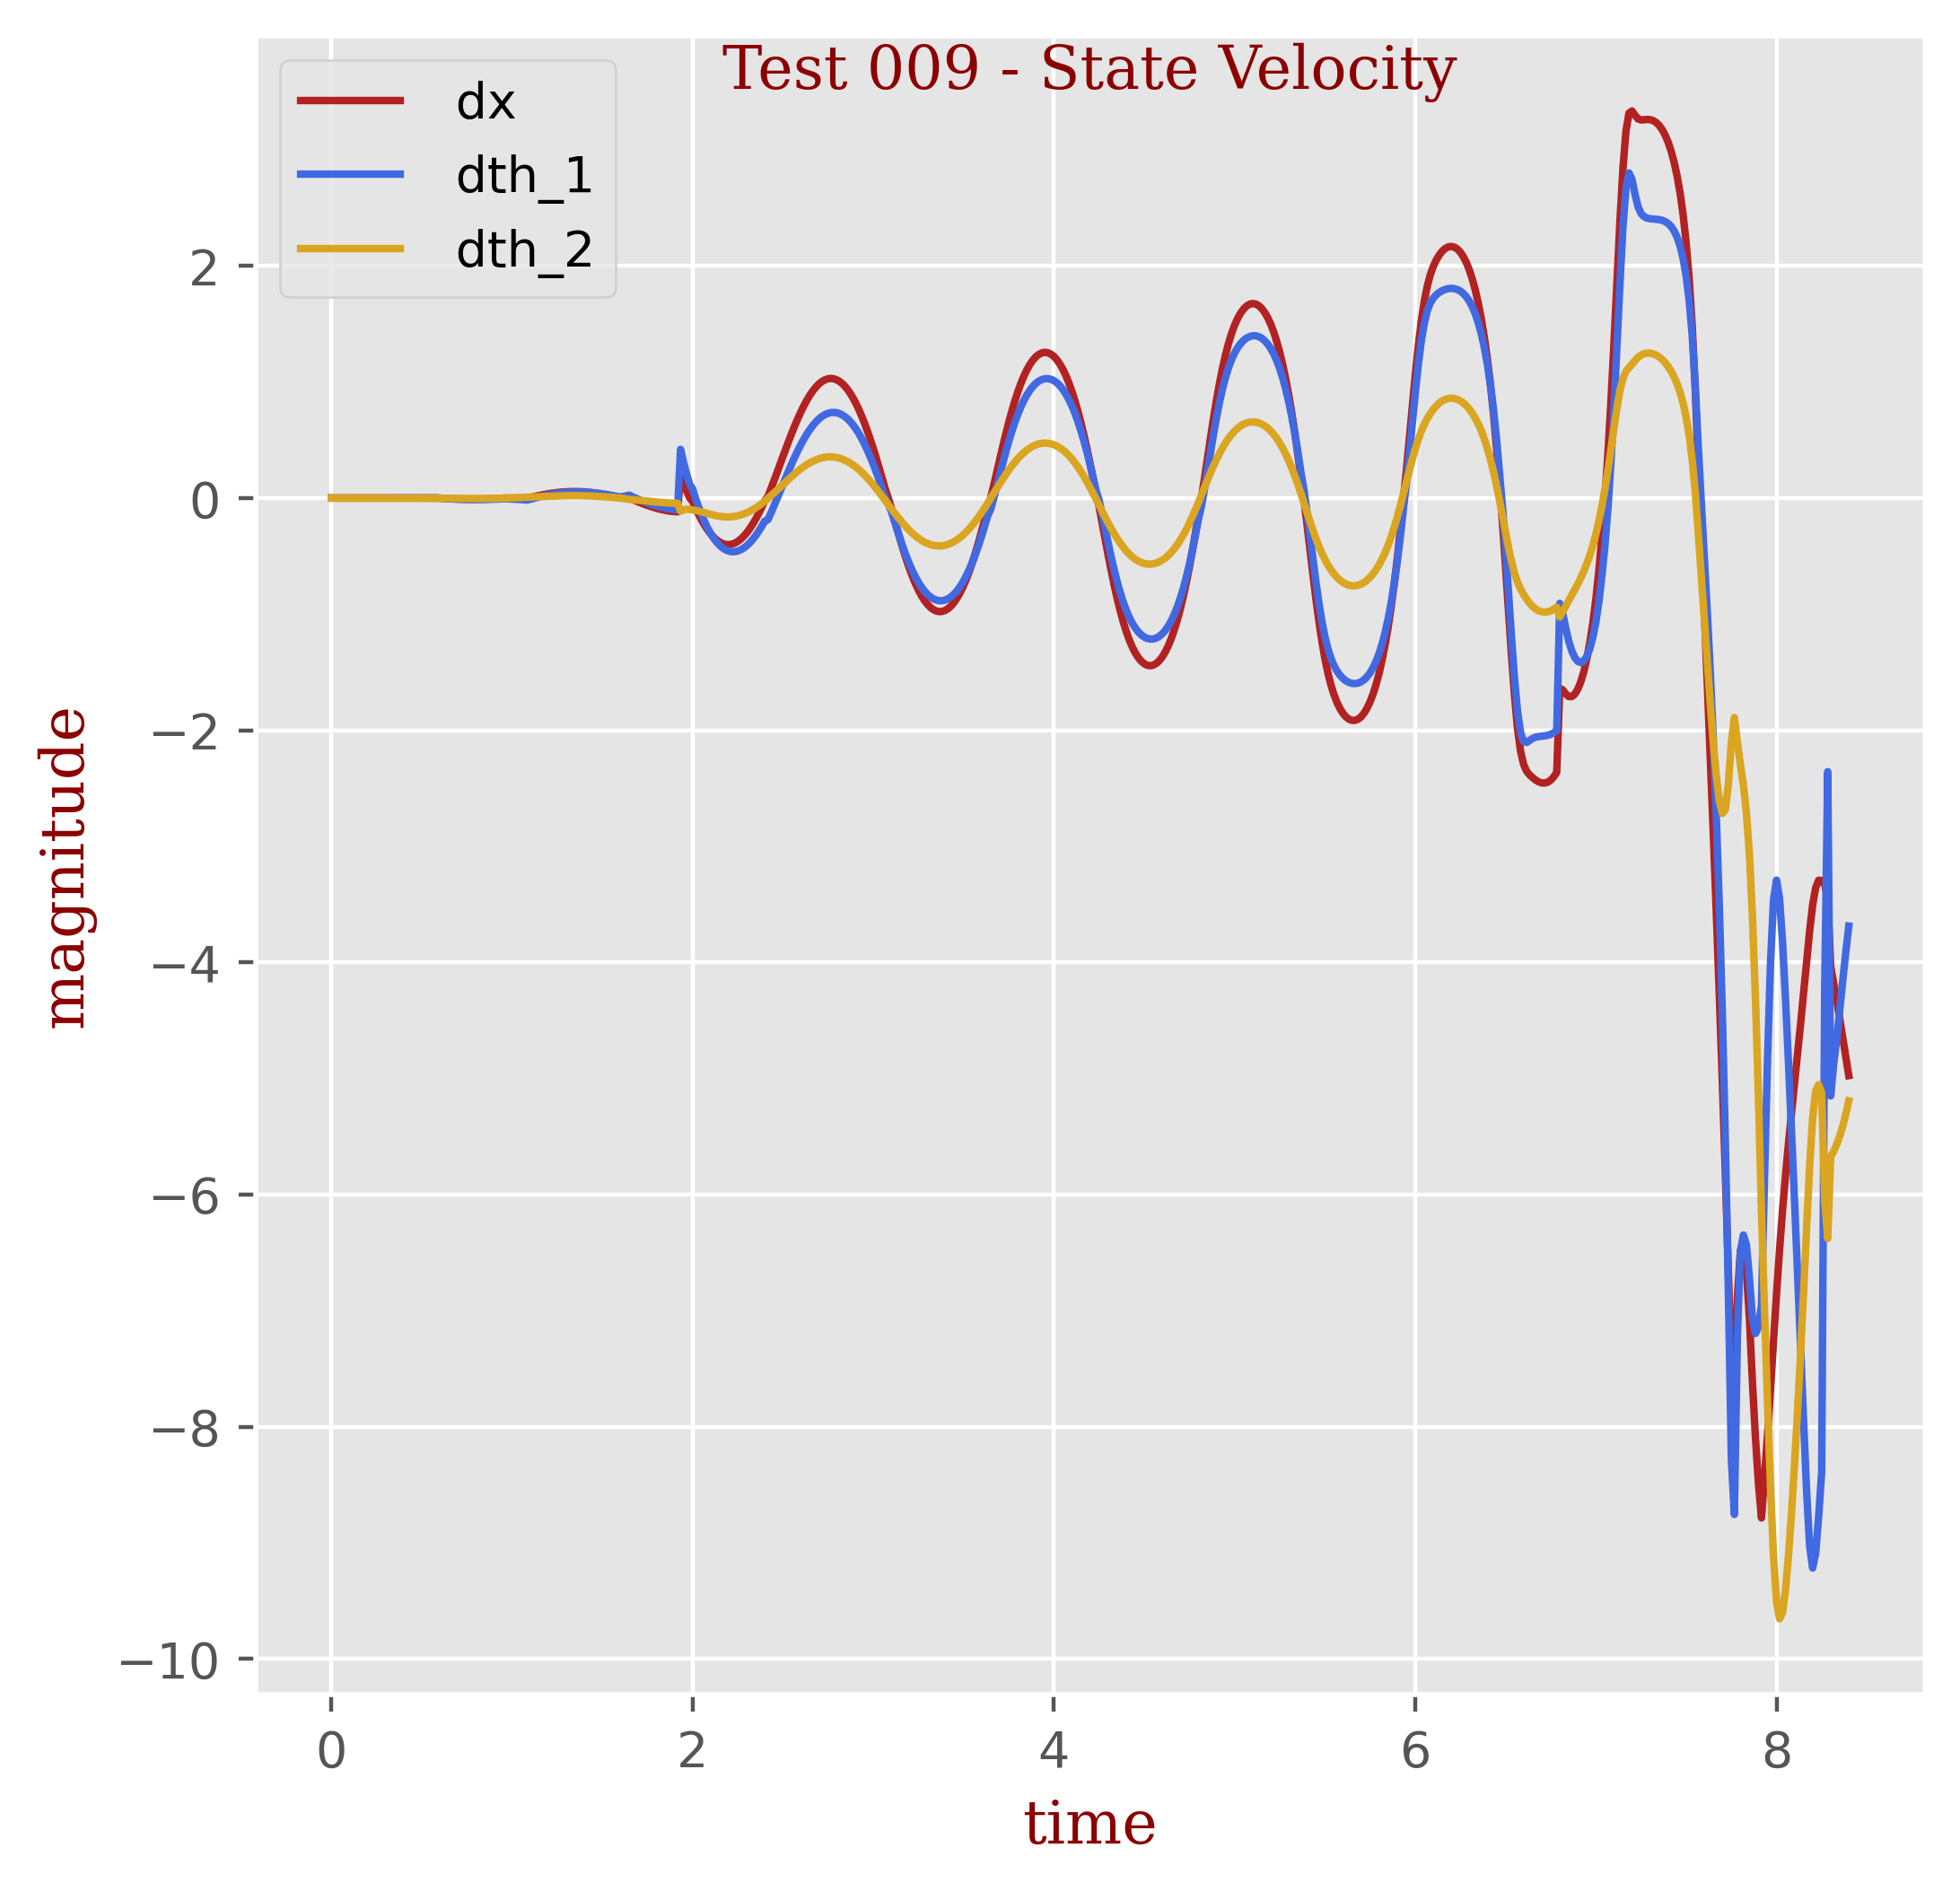
\includegraphics[width=27mm]{Test 009_State_Velocity.png}}
\subfigure[\(J(t)\)]{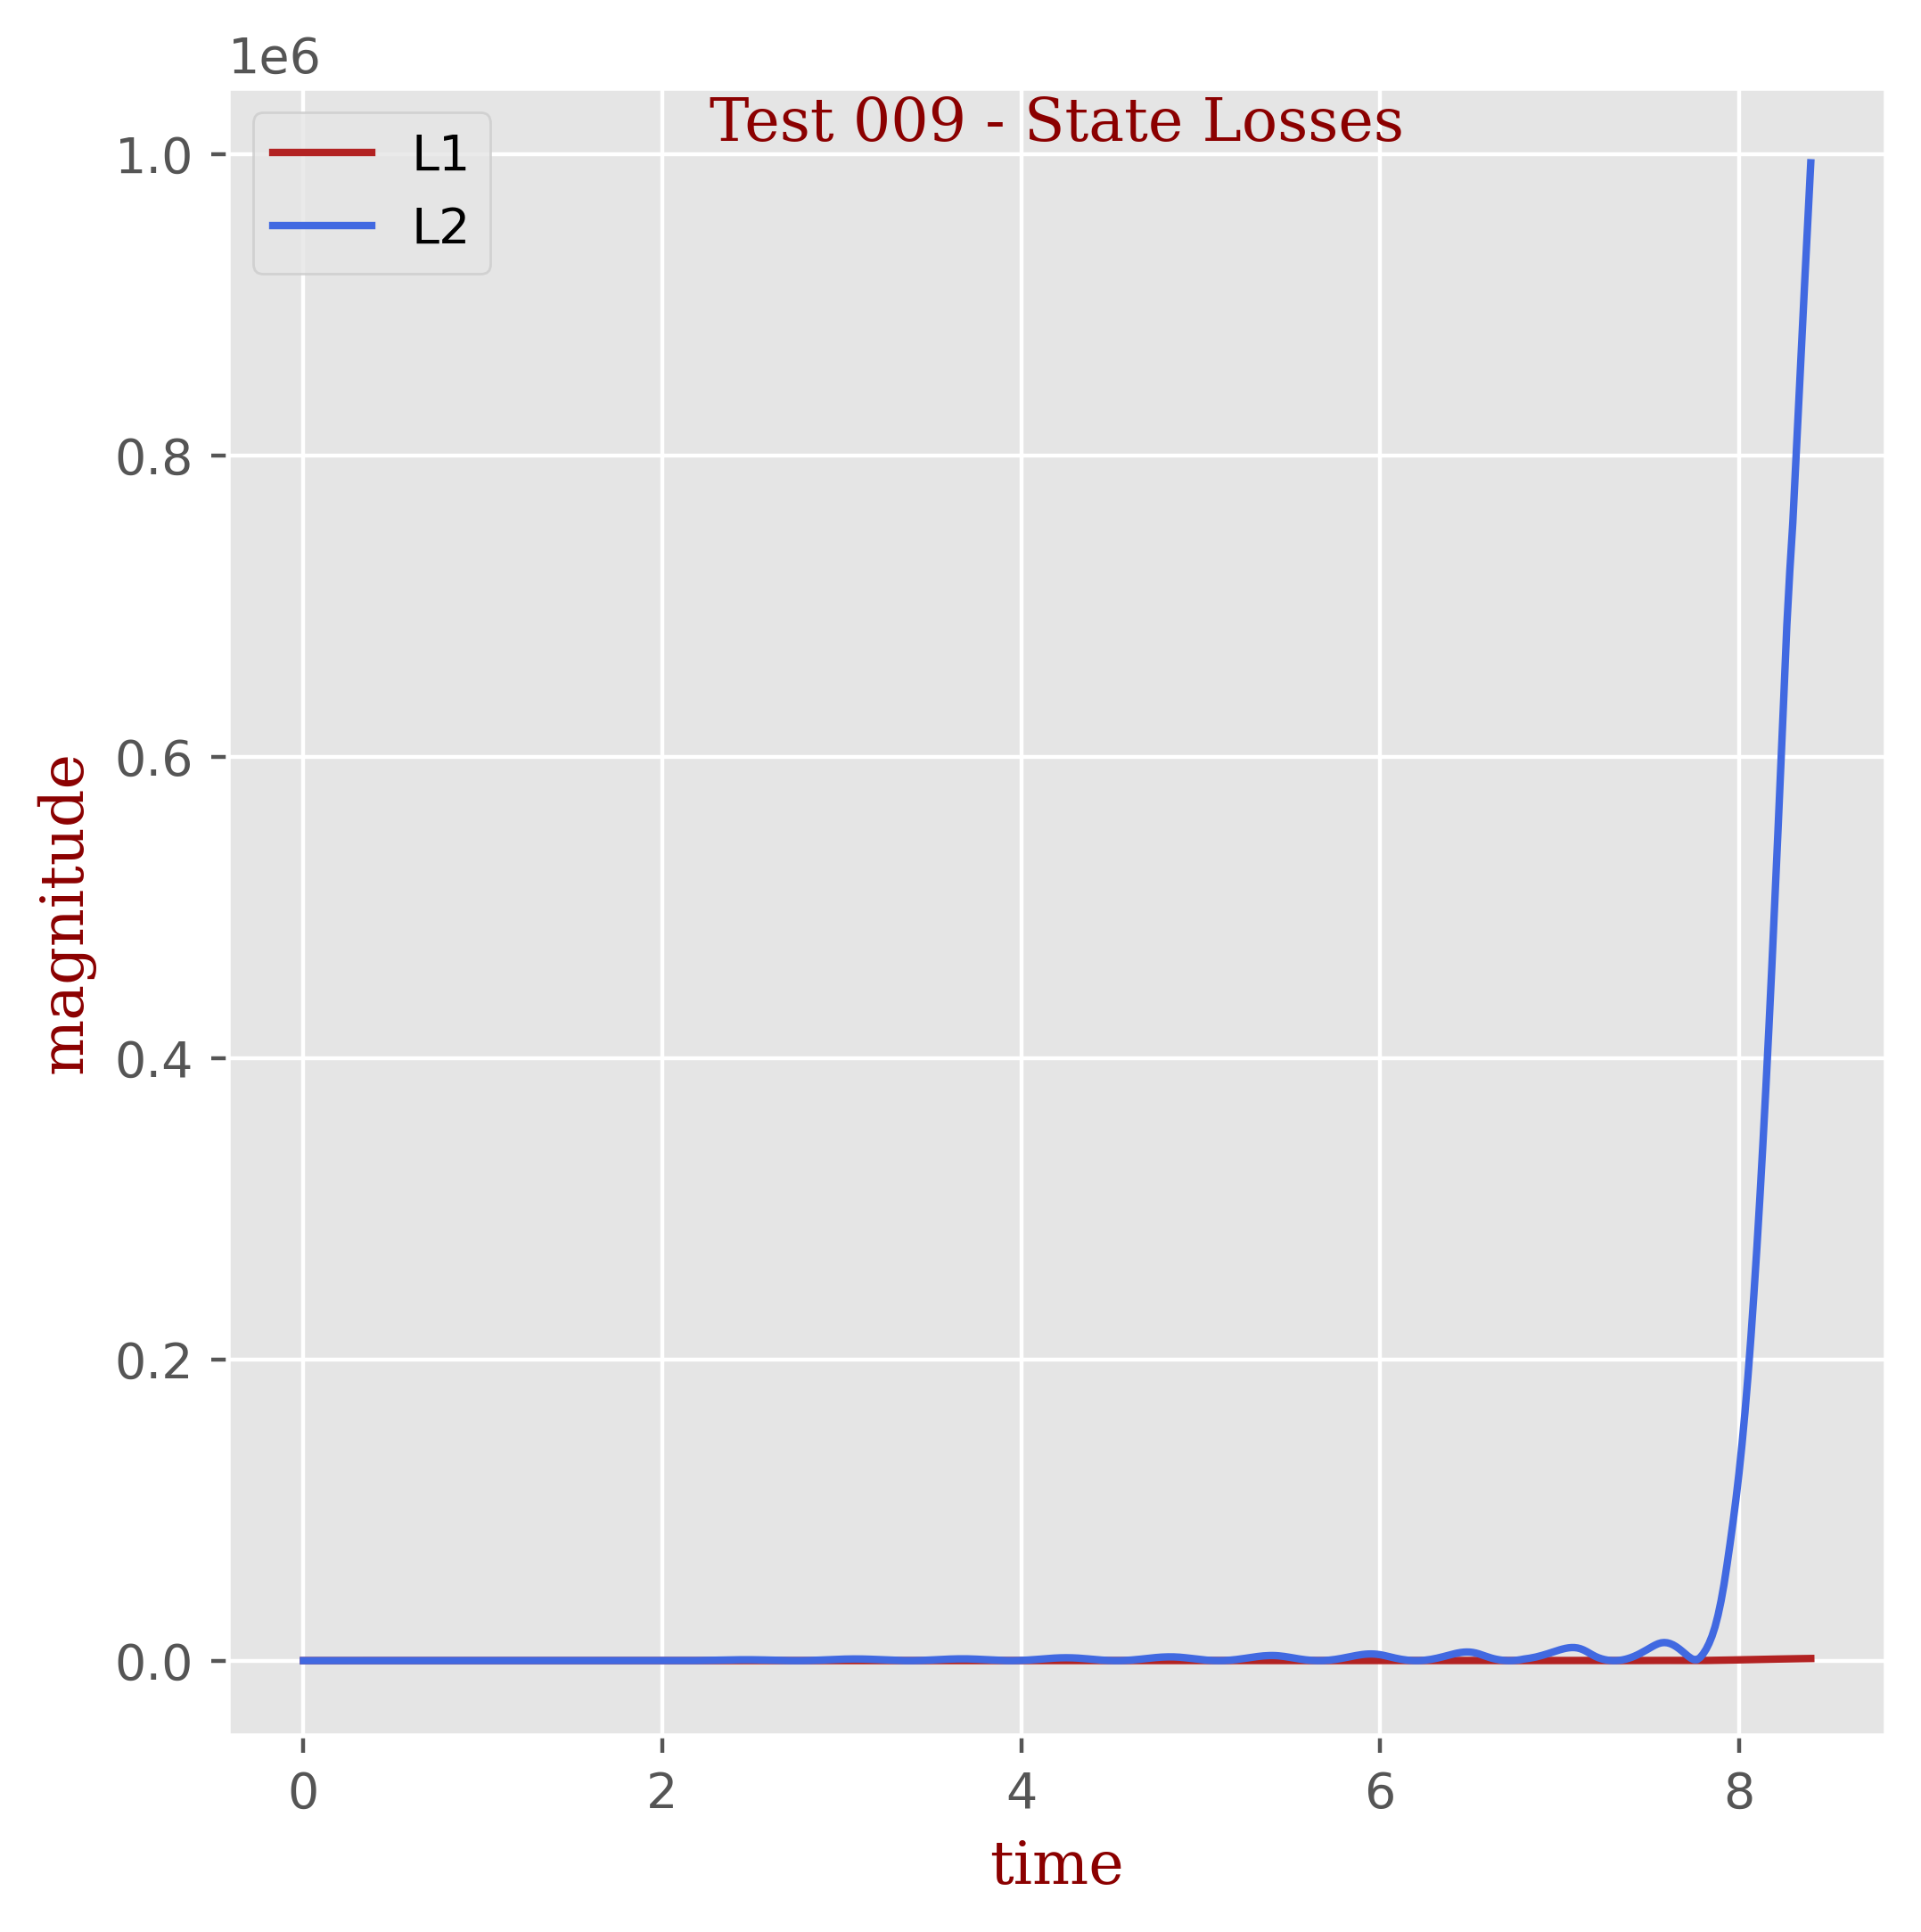
\includegraphics[width=27mm]{Test 009_State_Losses.png}}
\caption{Test 009}
\label{fig:t009}
\end{figure}

Tests 002-006 and 012 resulted in UUB stability and were bounded close to zero with
various bounds. Test 007 and 0013 were interesting due to their unique results.
Test 007 has heavier top and starts with a tighter bound and lower frequency
but after a few seconds it suddenly becomes unstable. Test 0013 has shorter
lower pendulum and moved violently from left to right to reach stability and
remained bounded throughout the duration of the test. Both cases are at the
margin of UUB stability; thus, we named it \emph{marginal-UUB}.
Tests 008-010 and 014 were unstable.





\begin{figure}
\centering
\subfigure[\(q(t)\)]{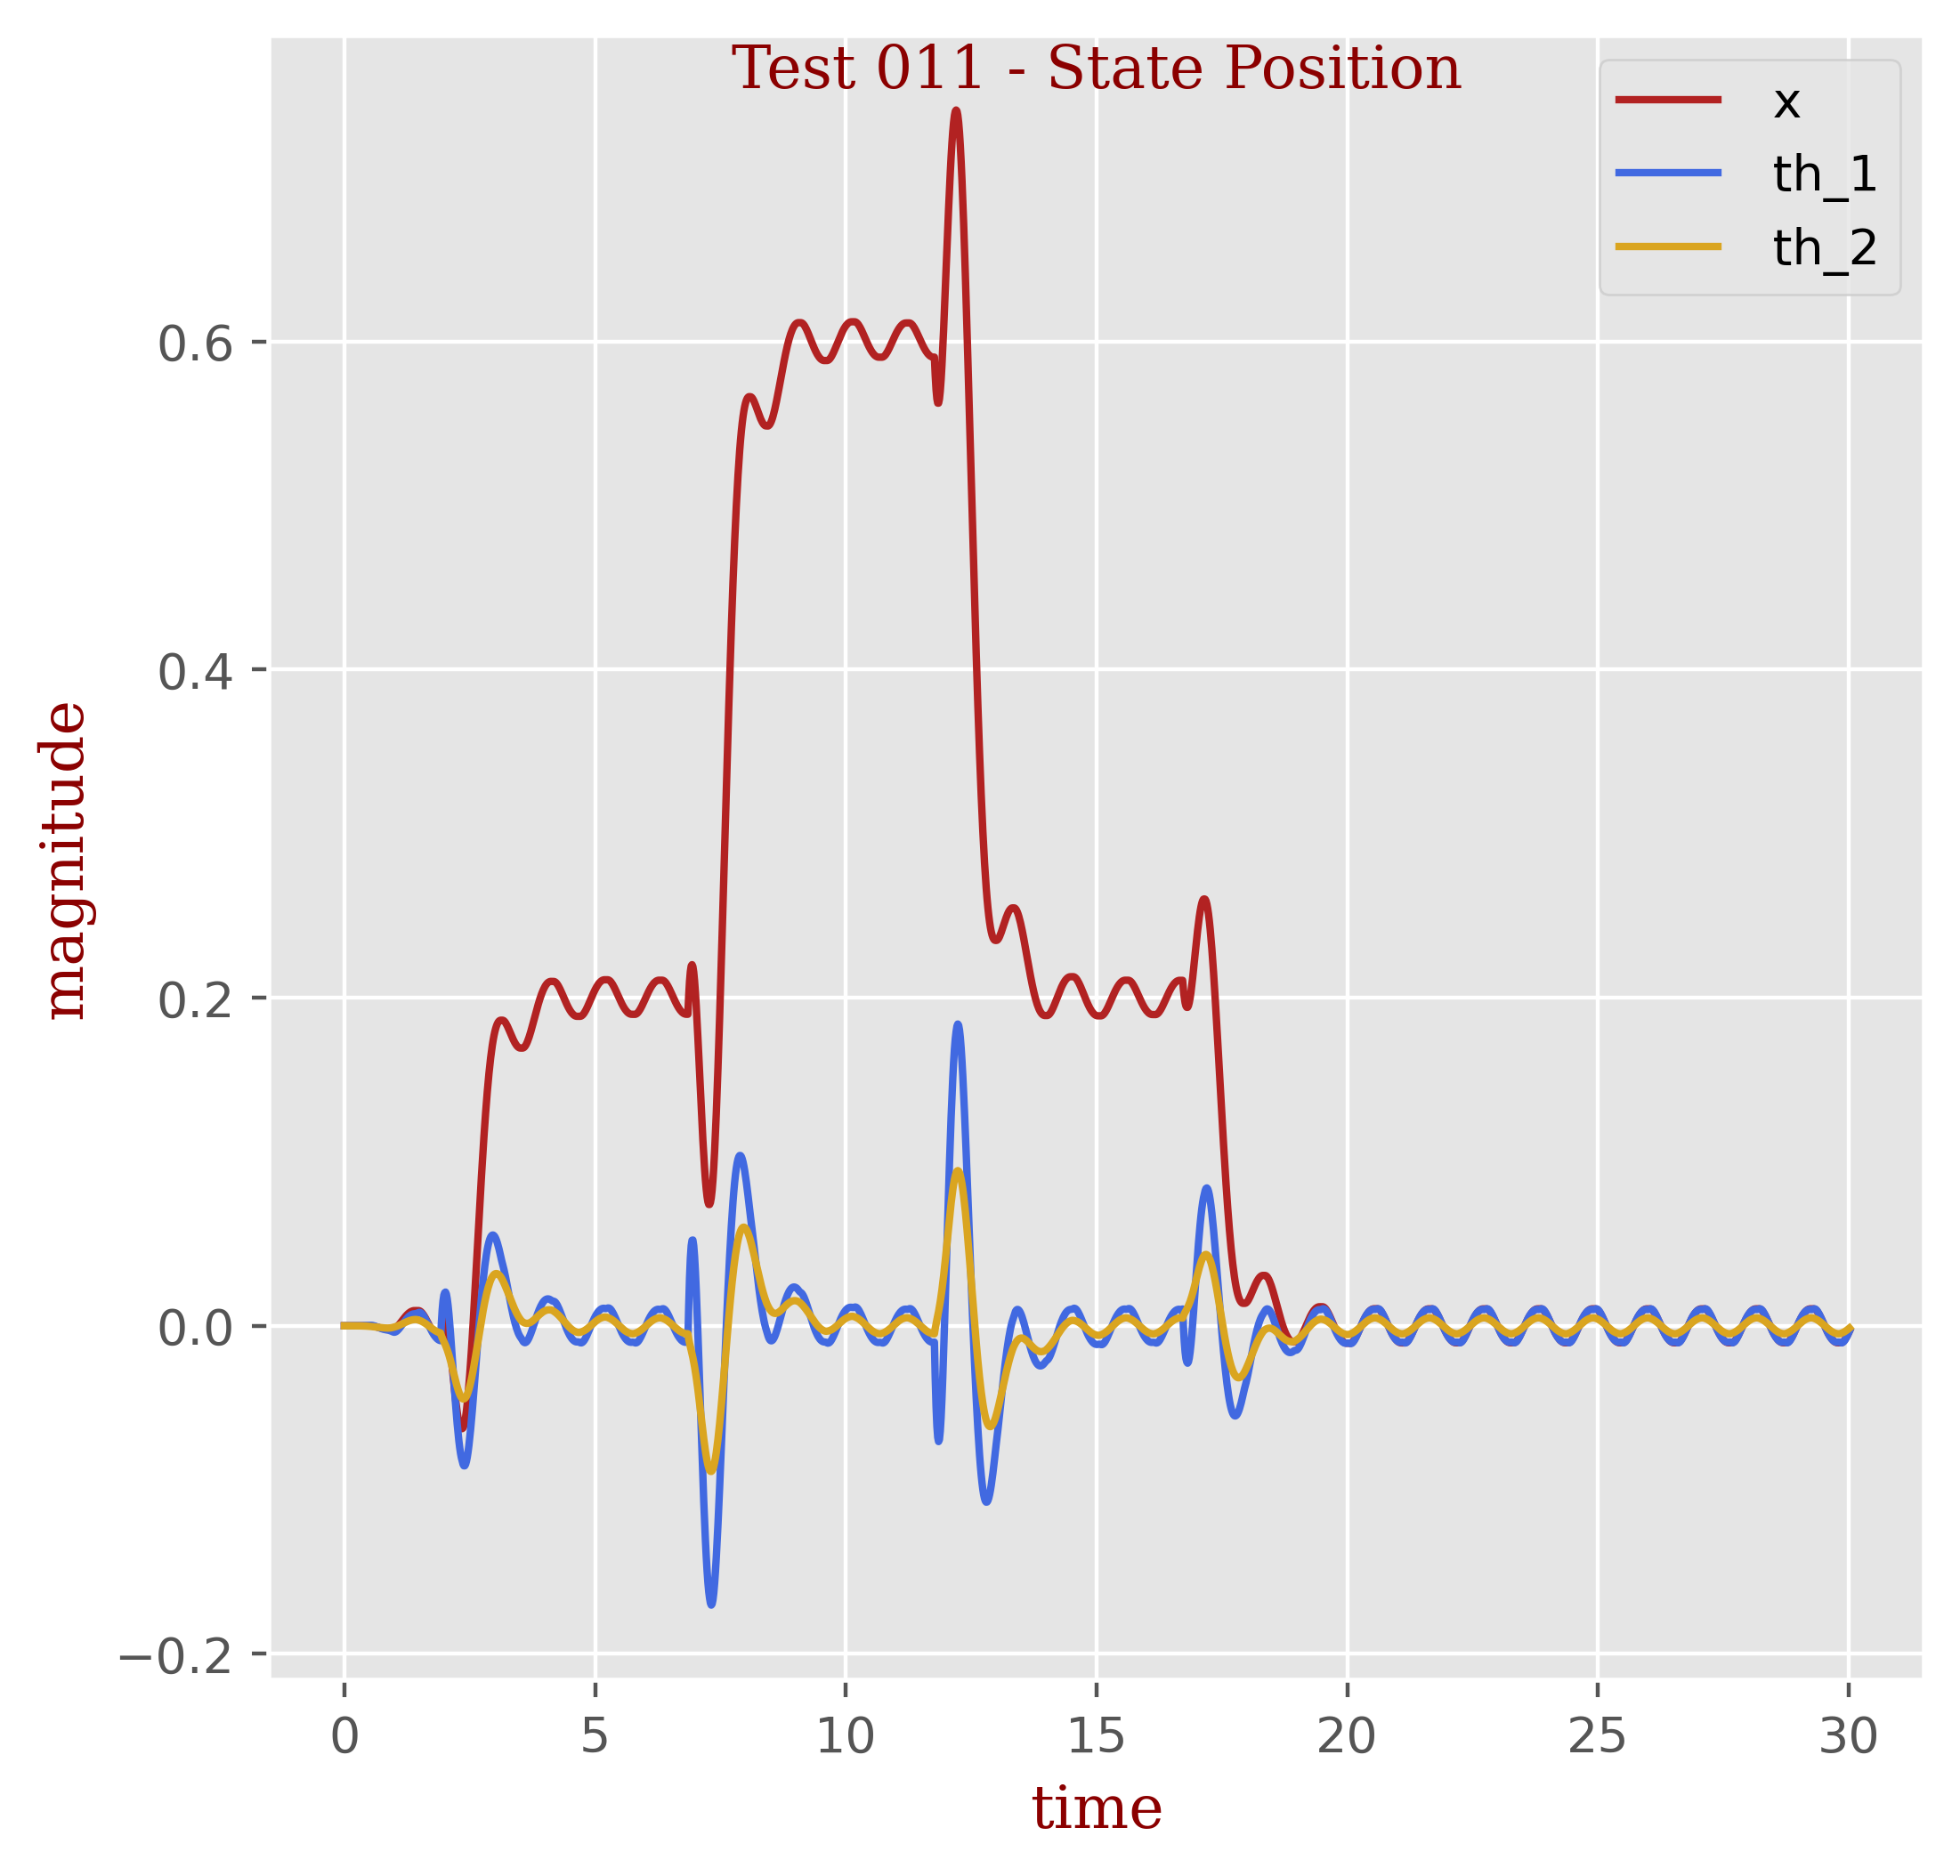
\includegraphics[width=27mm]{Test 011_State_Position.png}}
\subfigure[\(\dot{q}(t)\)]{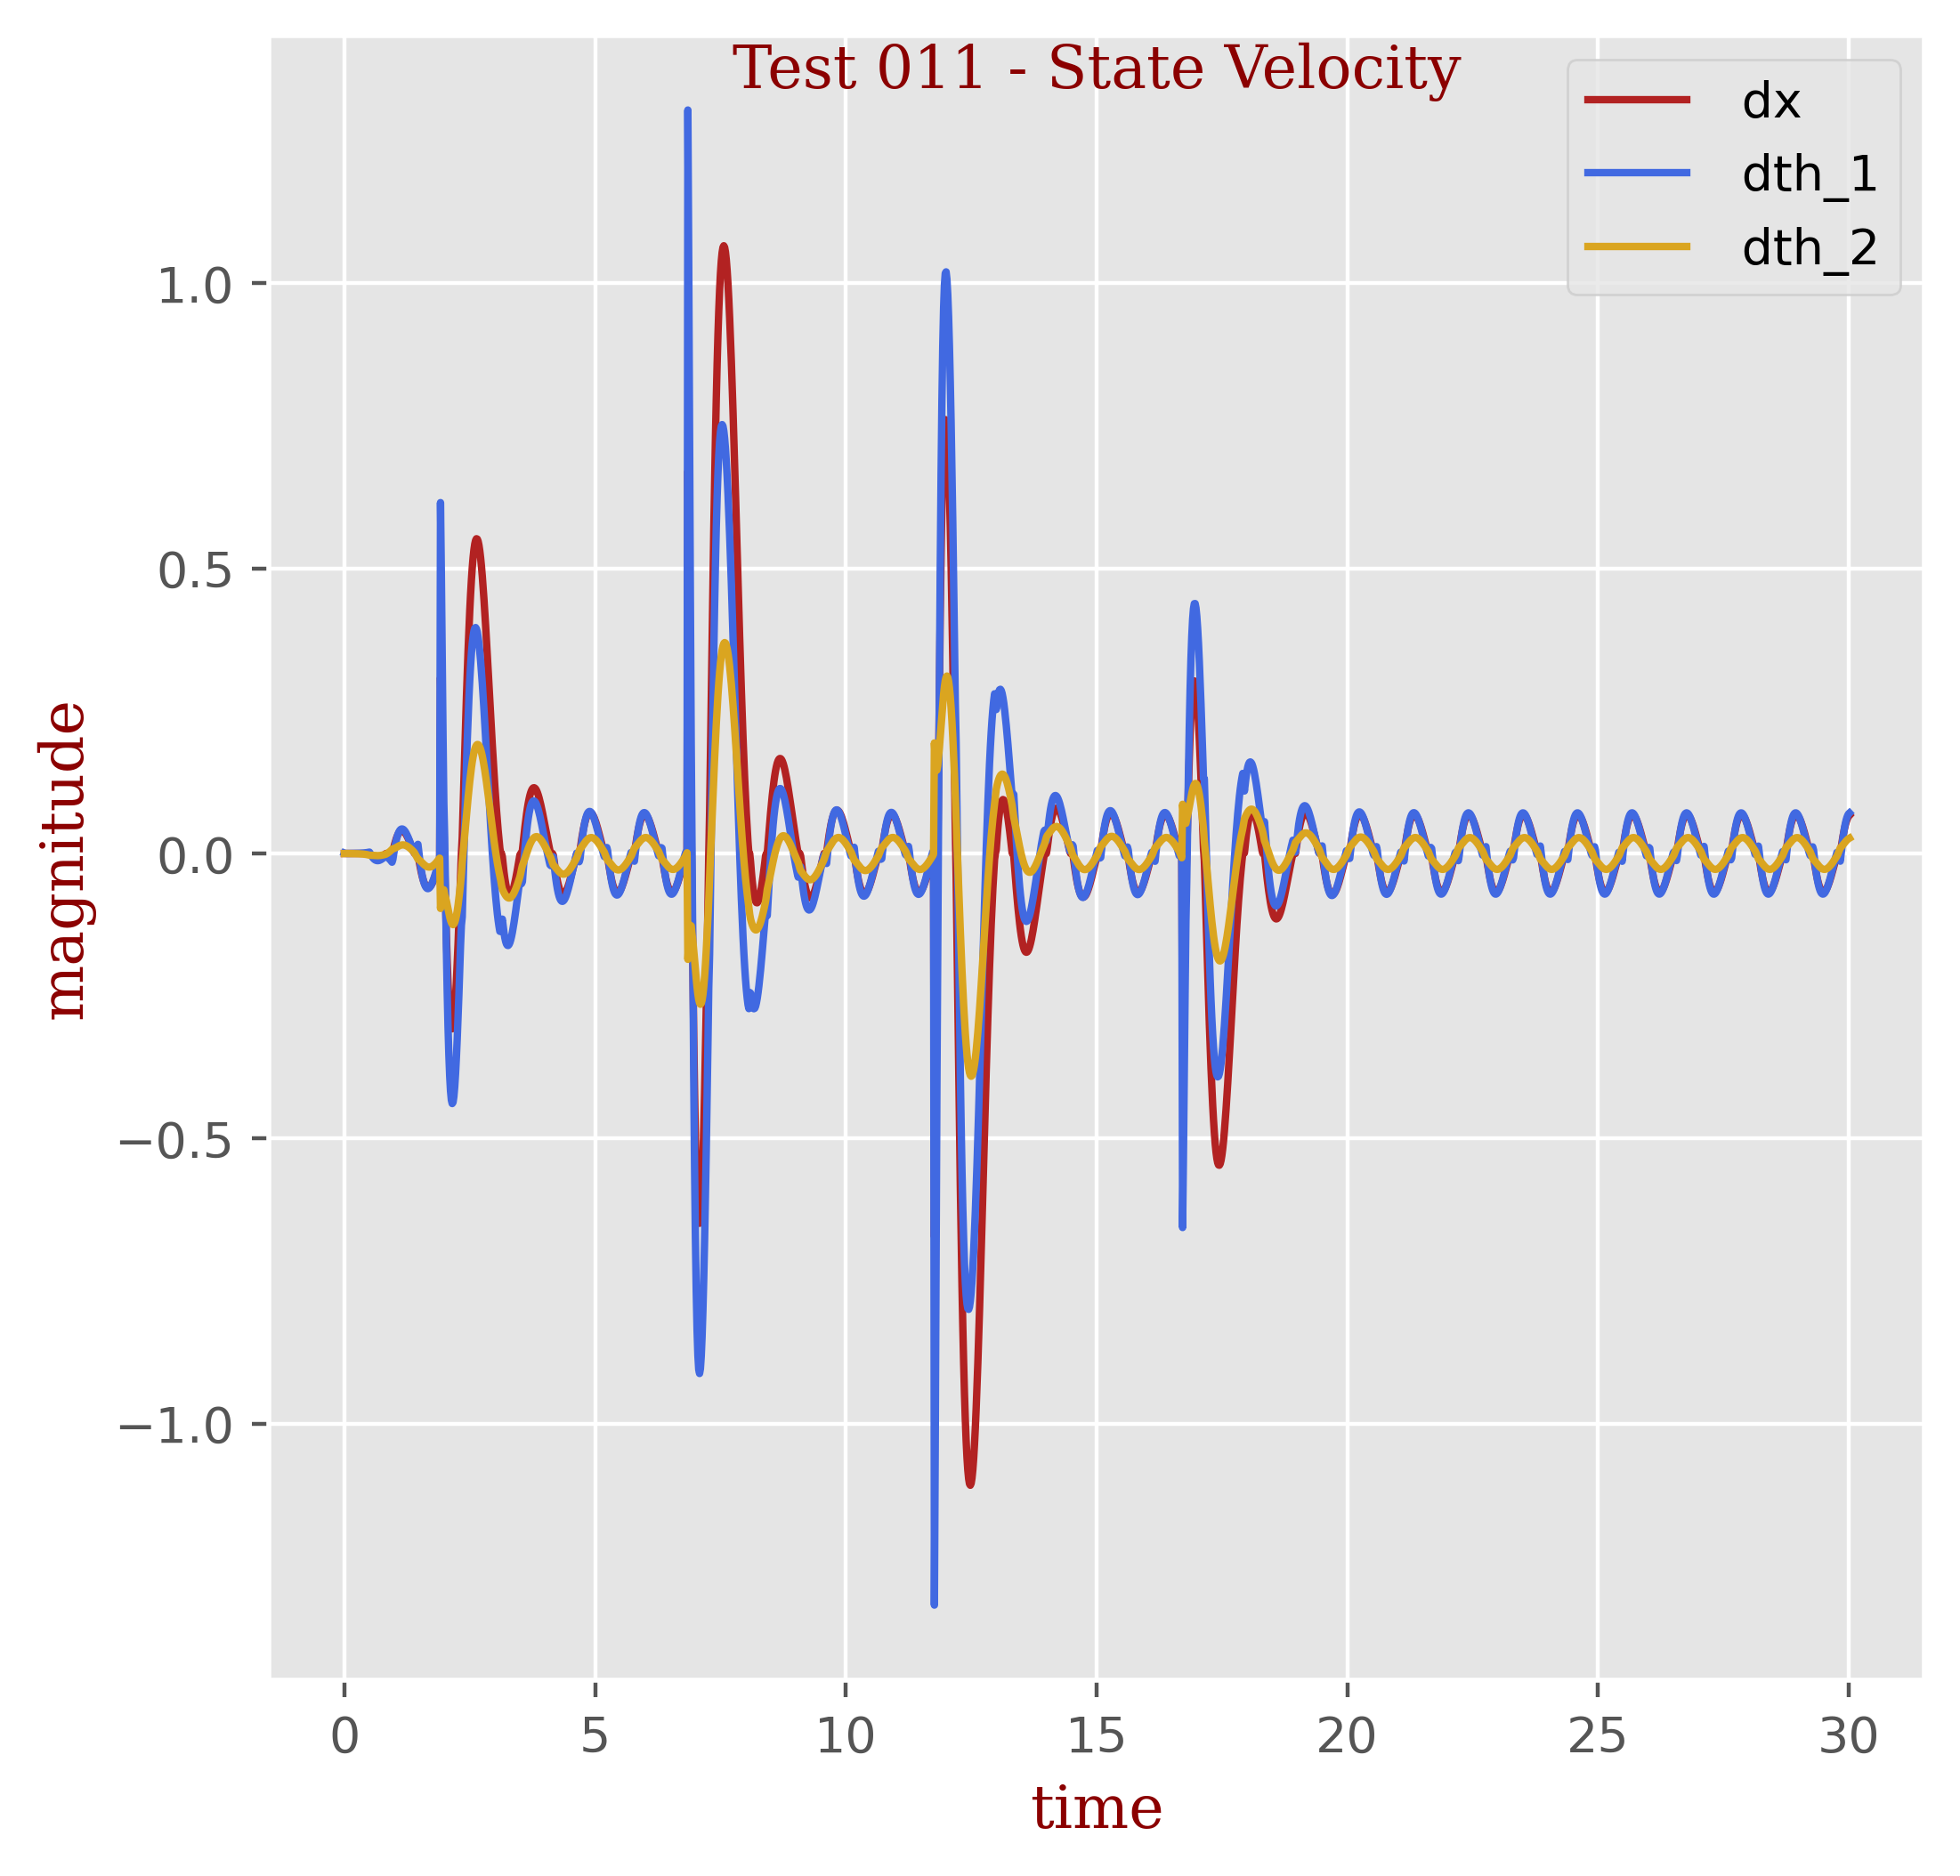
\includegraphics[width=27mm]{Test 011_State_Velocity.png}}
\subfigure[\(J(t)\)]{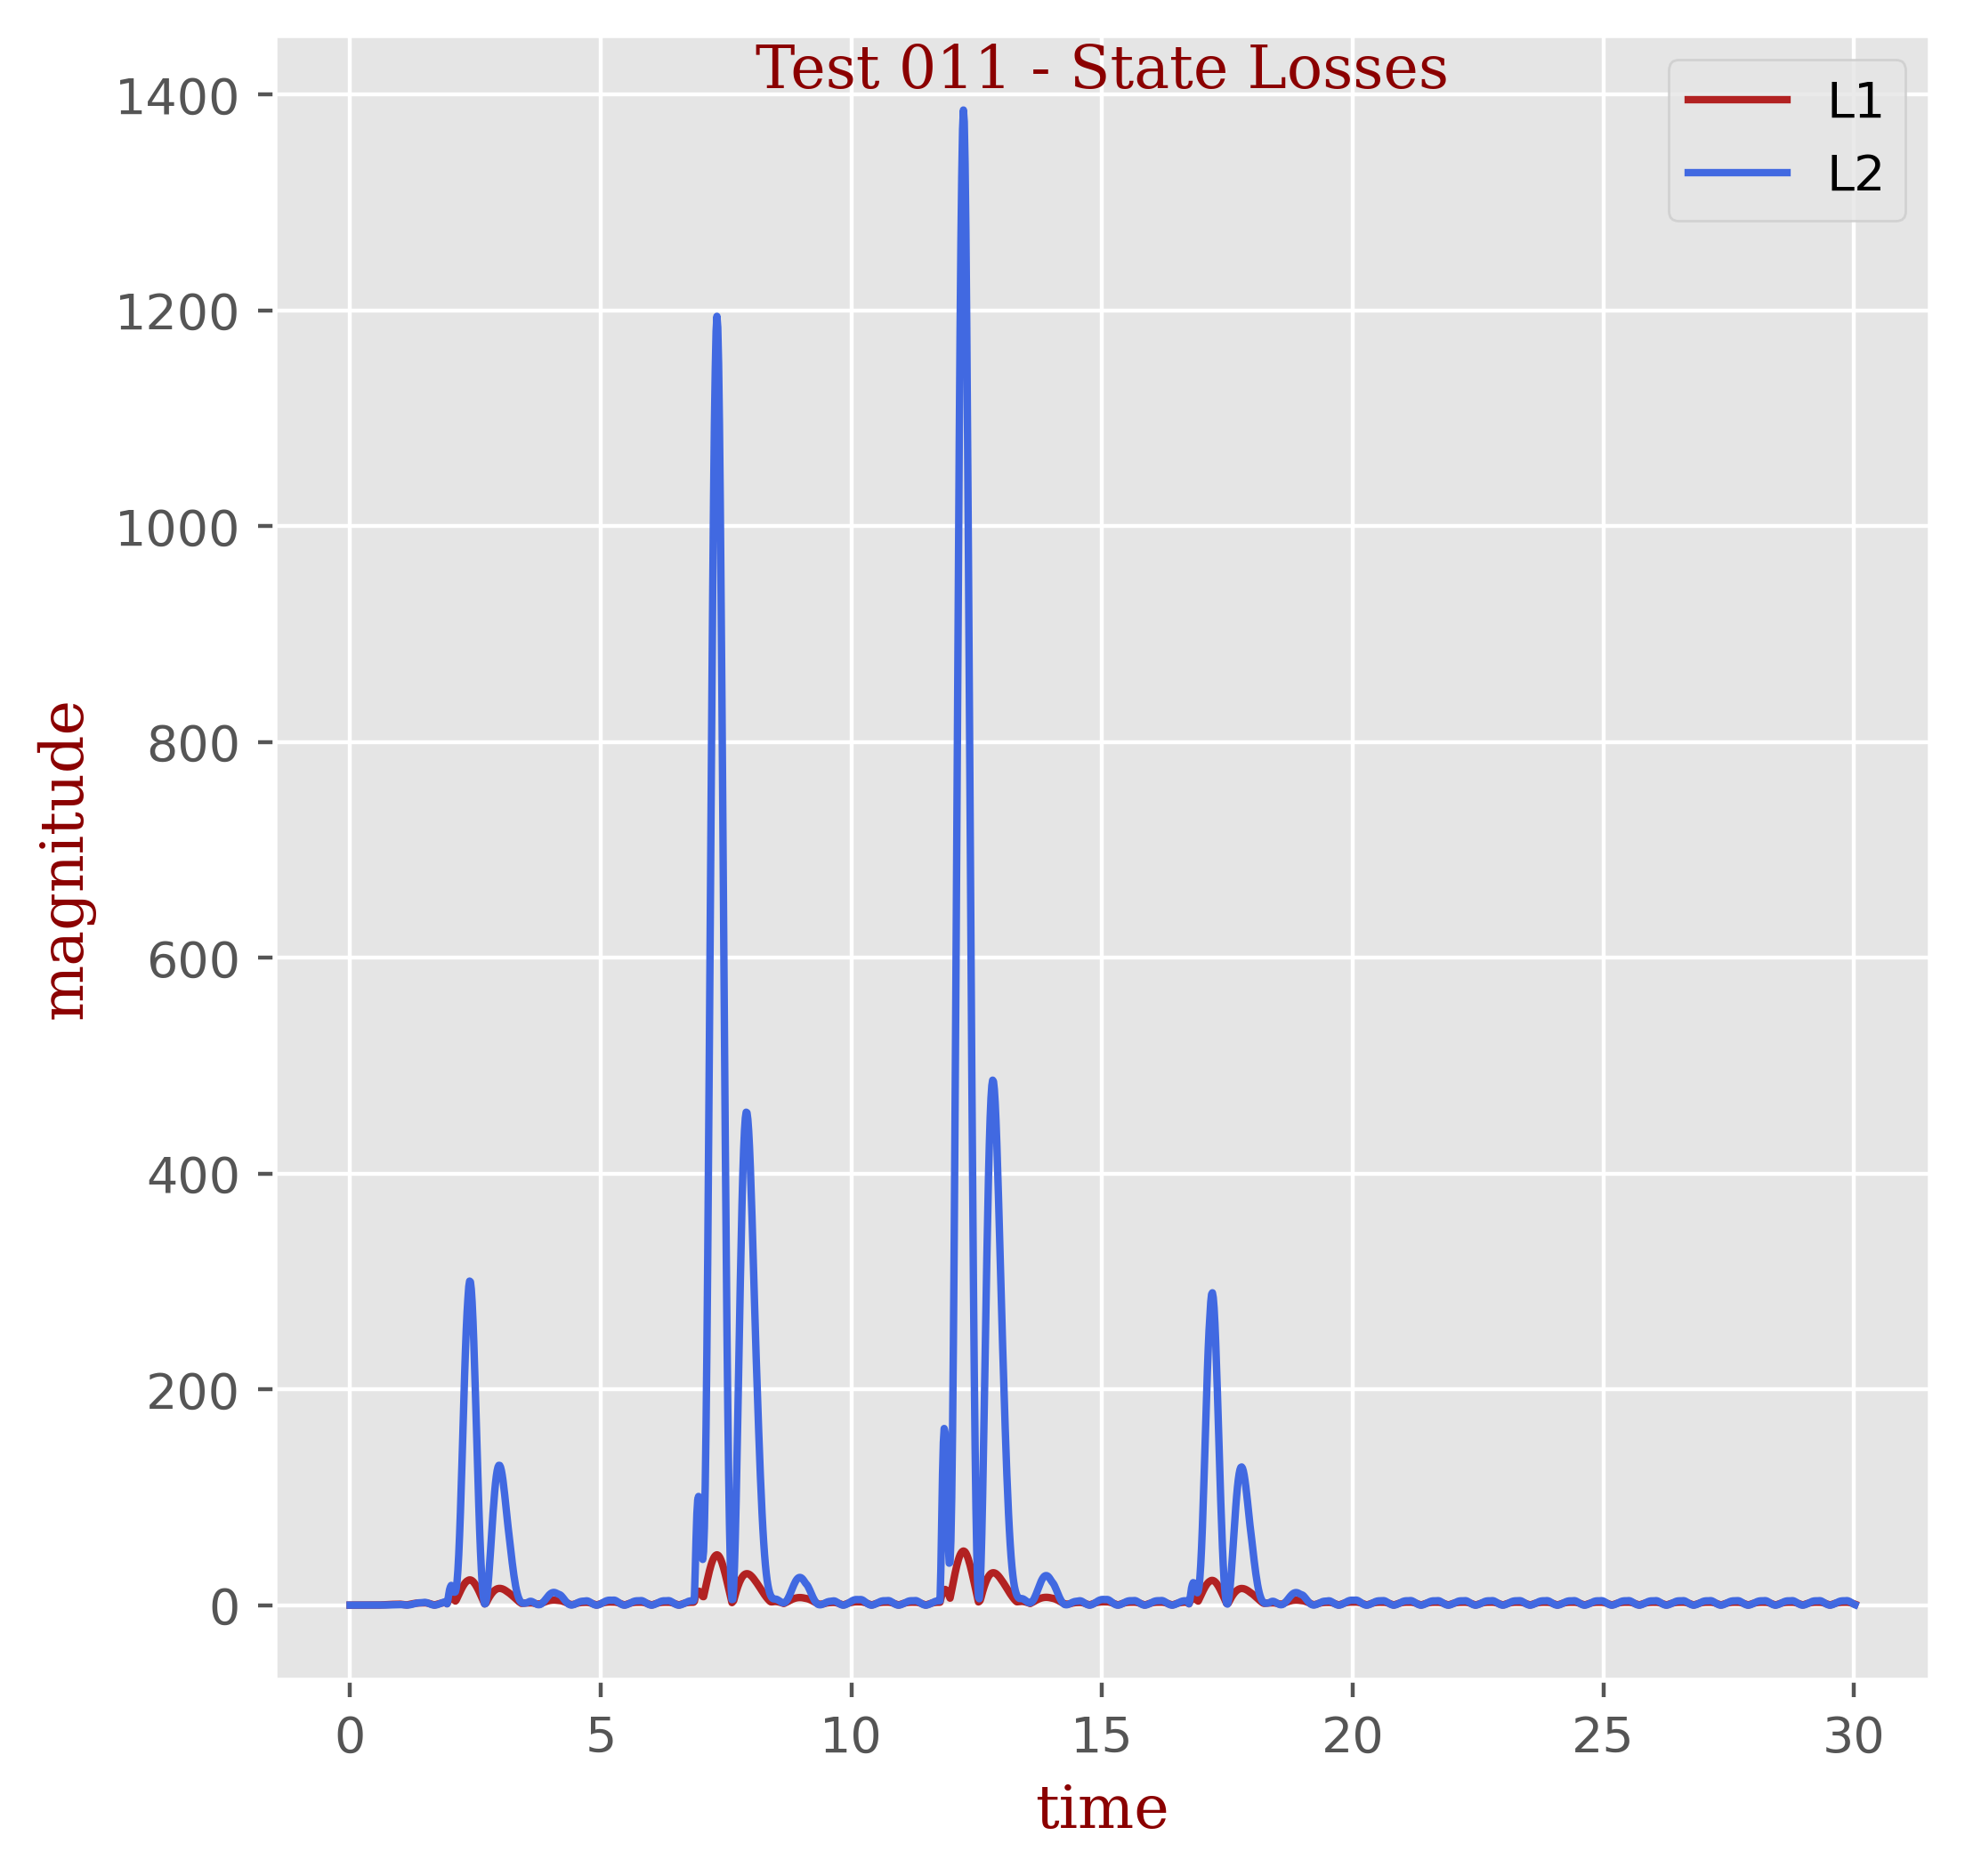
\includegraphics[width=27mm]{Test 011_State_Losses.png}}
\caption{Test 011}
\label{fig:t011}
\end{figure}



\begin{figure}
\centering
\subfigure[\(q(t)\)]{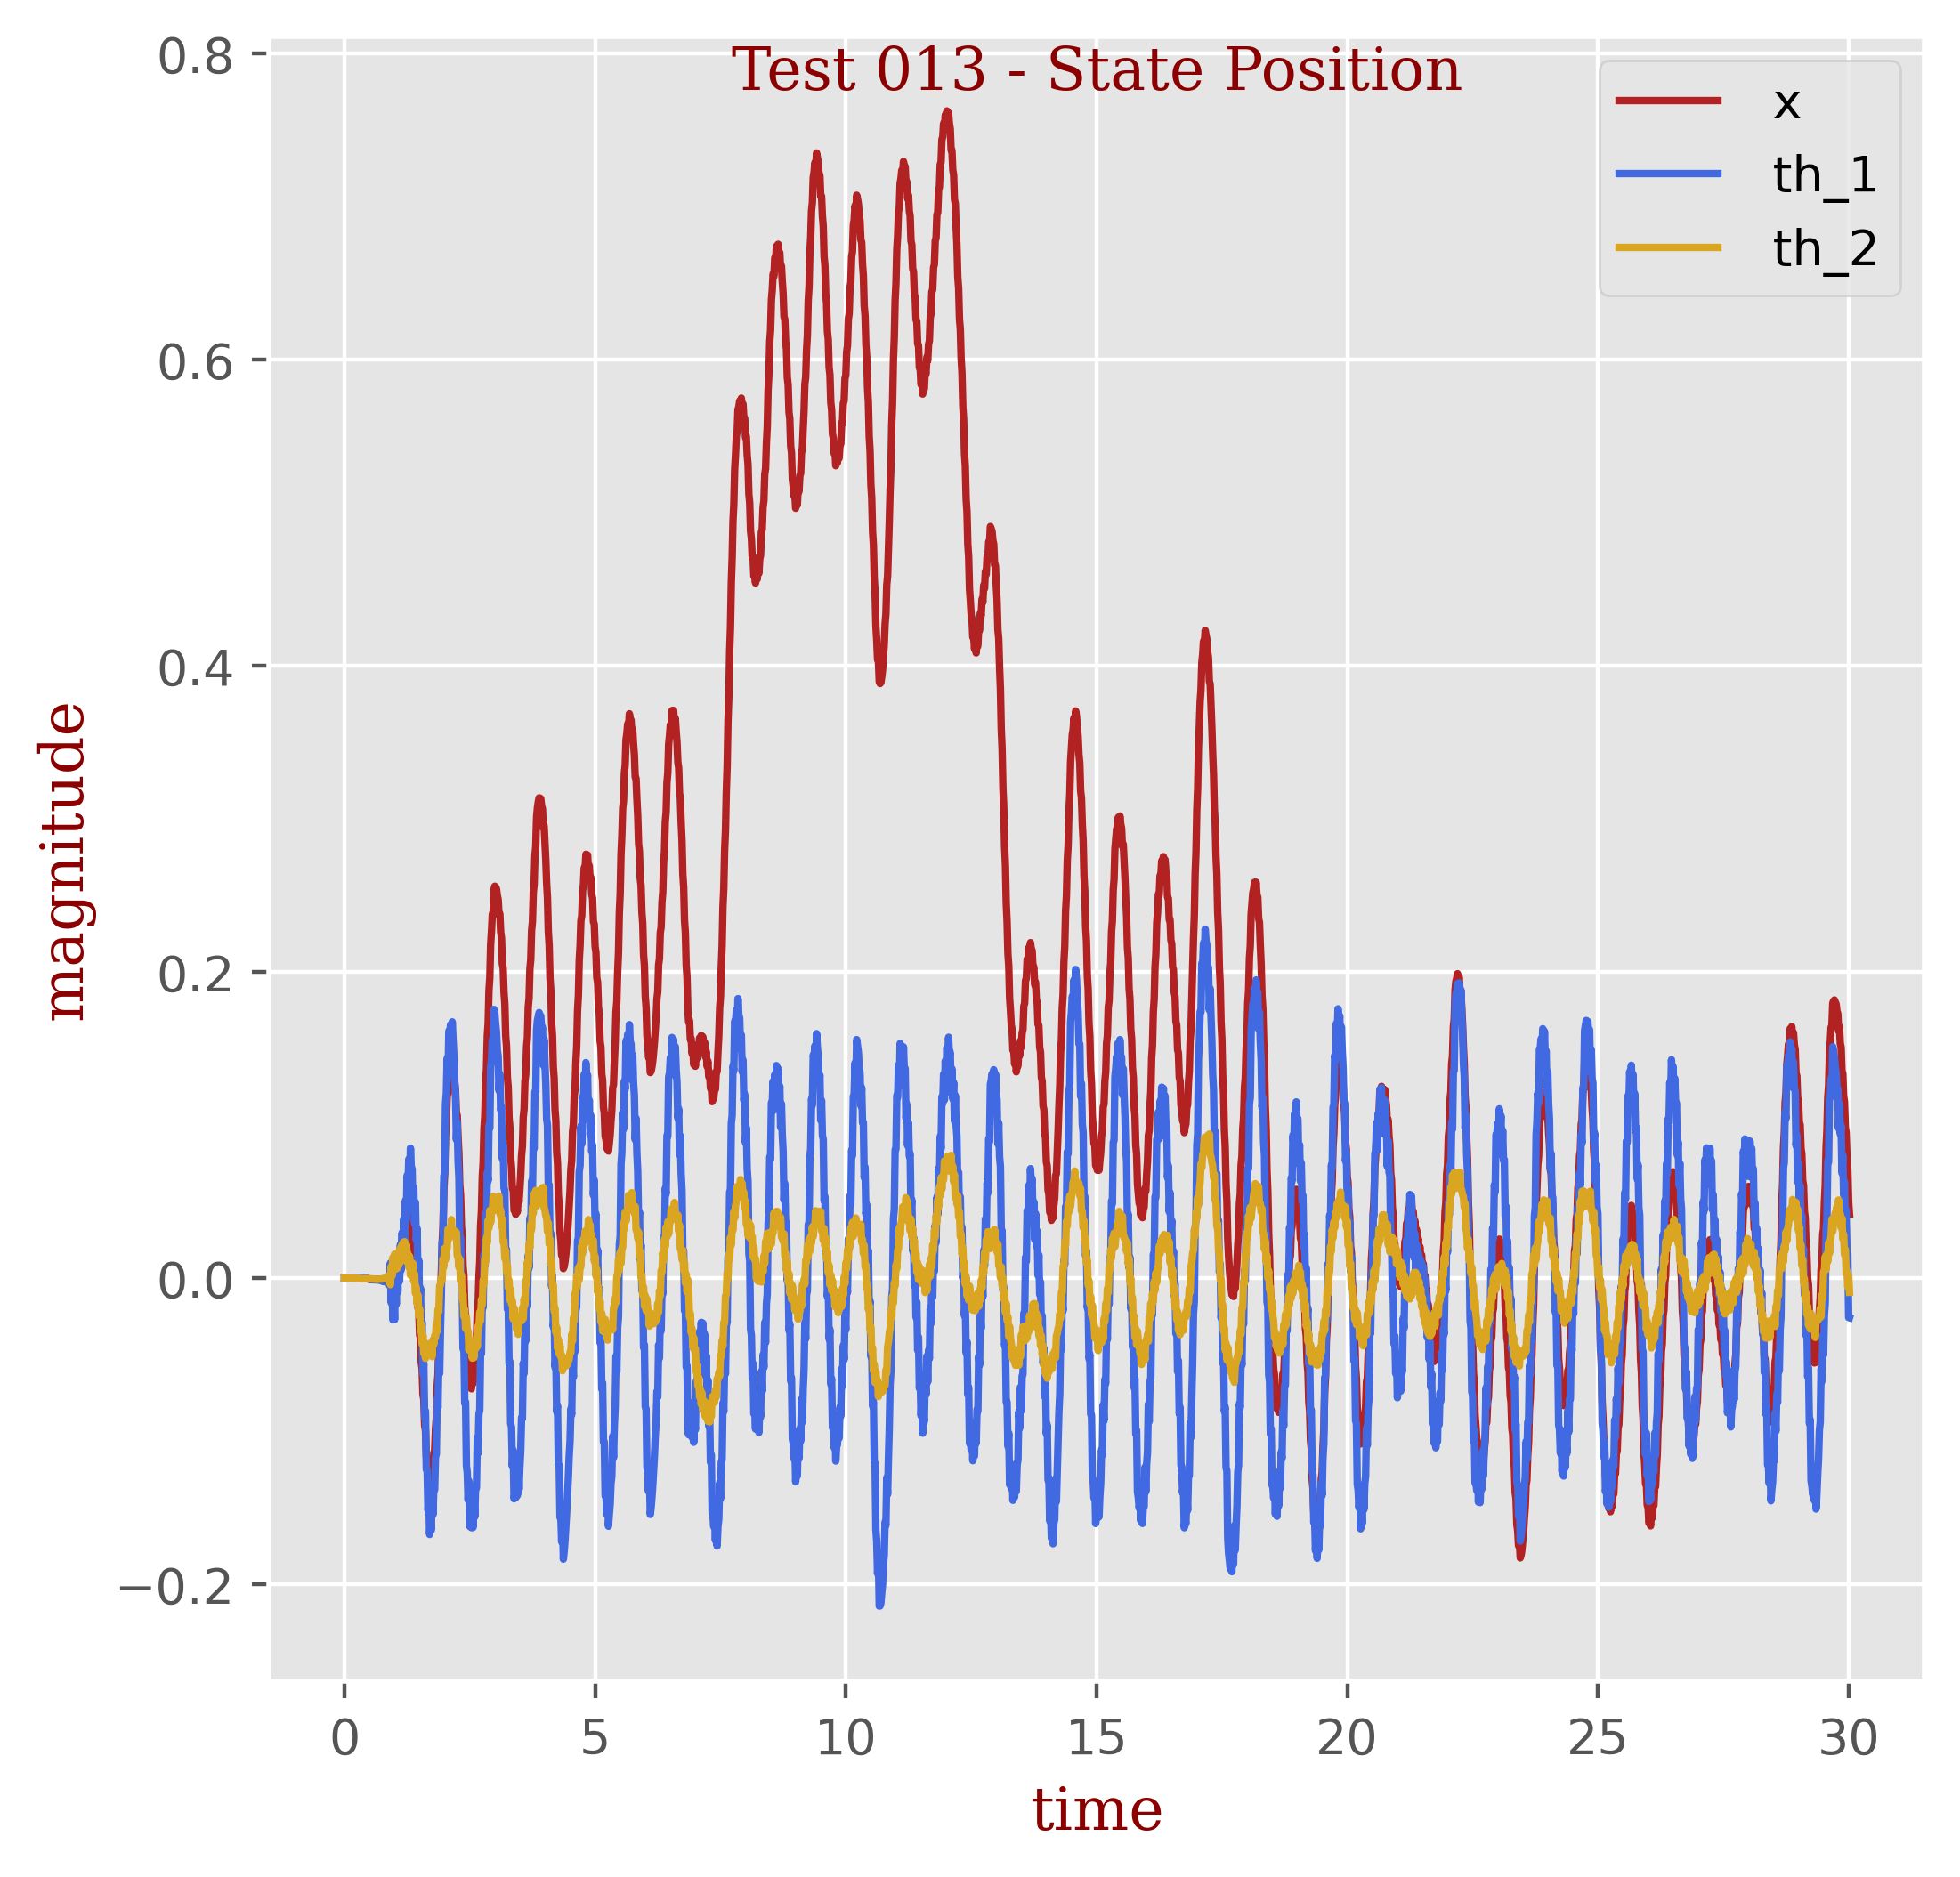
\includegraphics[width=27mm]{Test 013_State_Position.png}}
\subfigure[\(\dot{q}(t)\)]{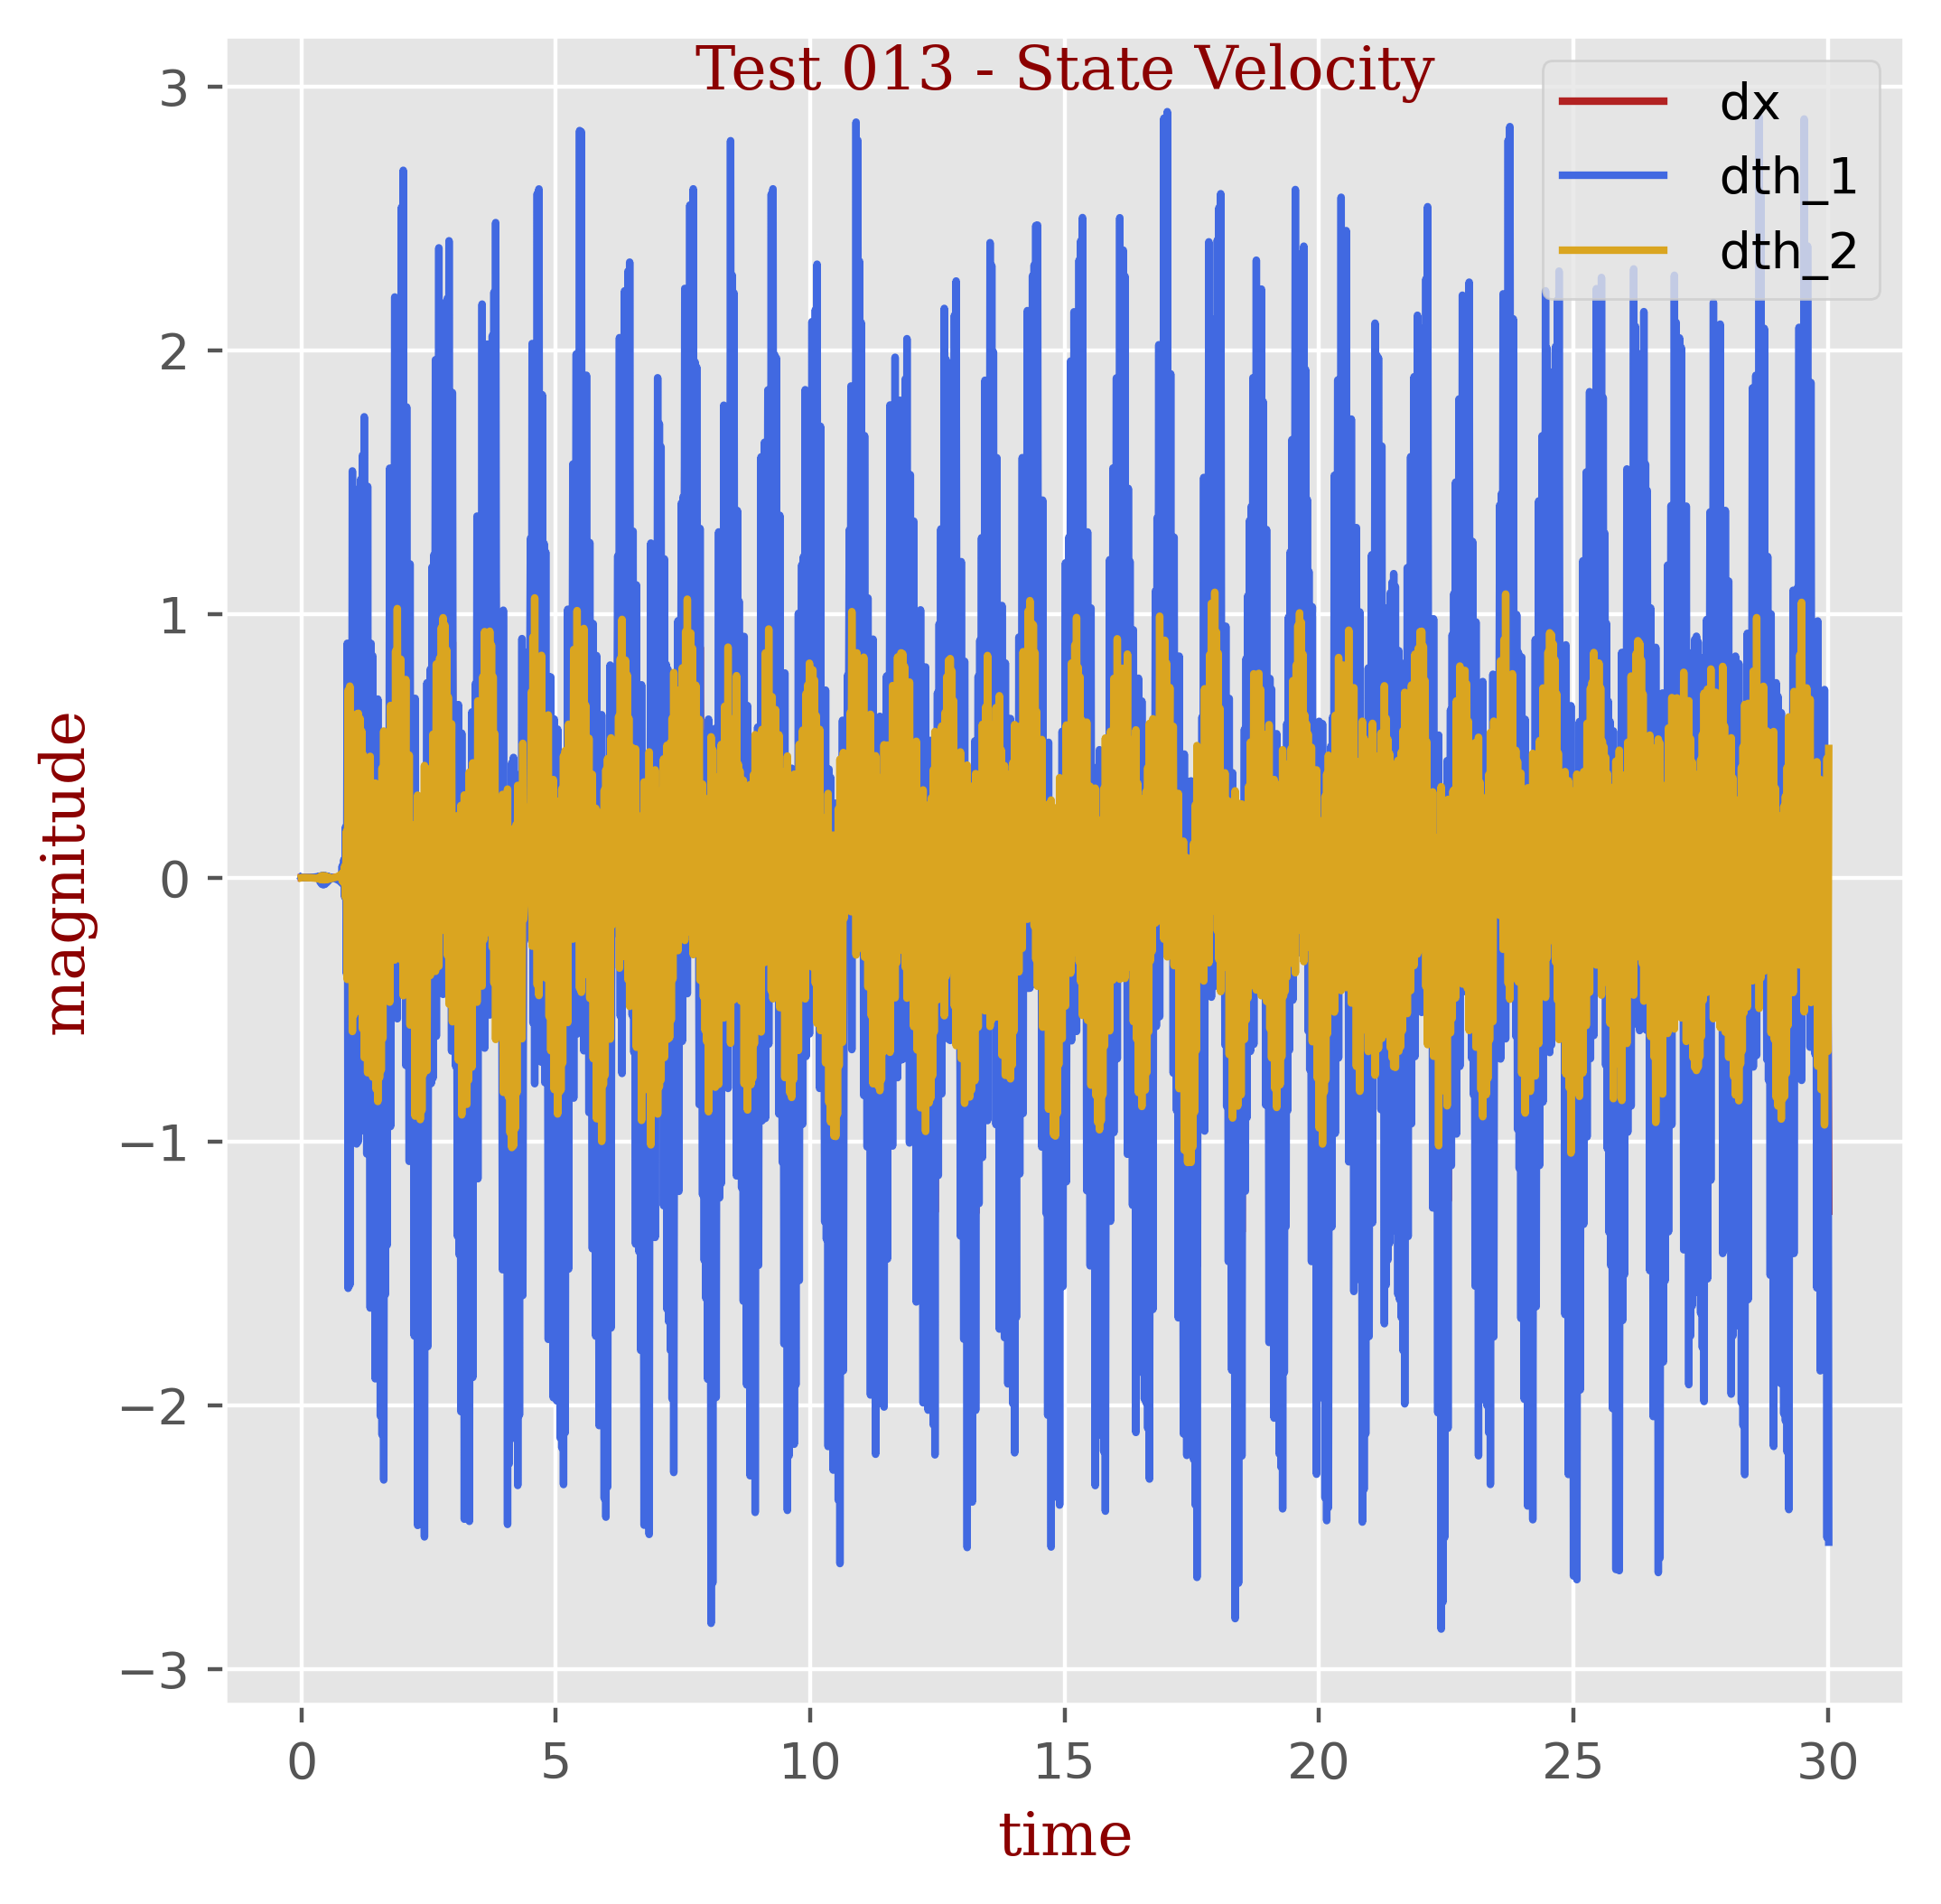
\includegraphics[width=27mm]{Test 013_State_Velocity.png}}
\subfigure[\(J(t)\)]{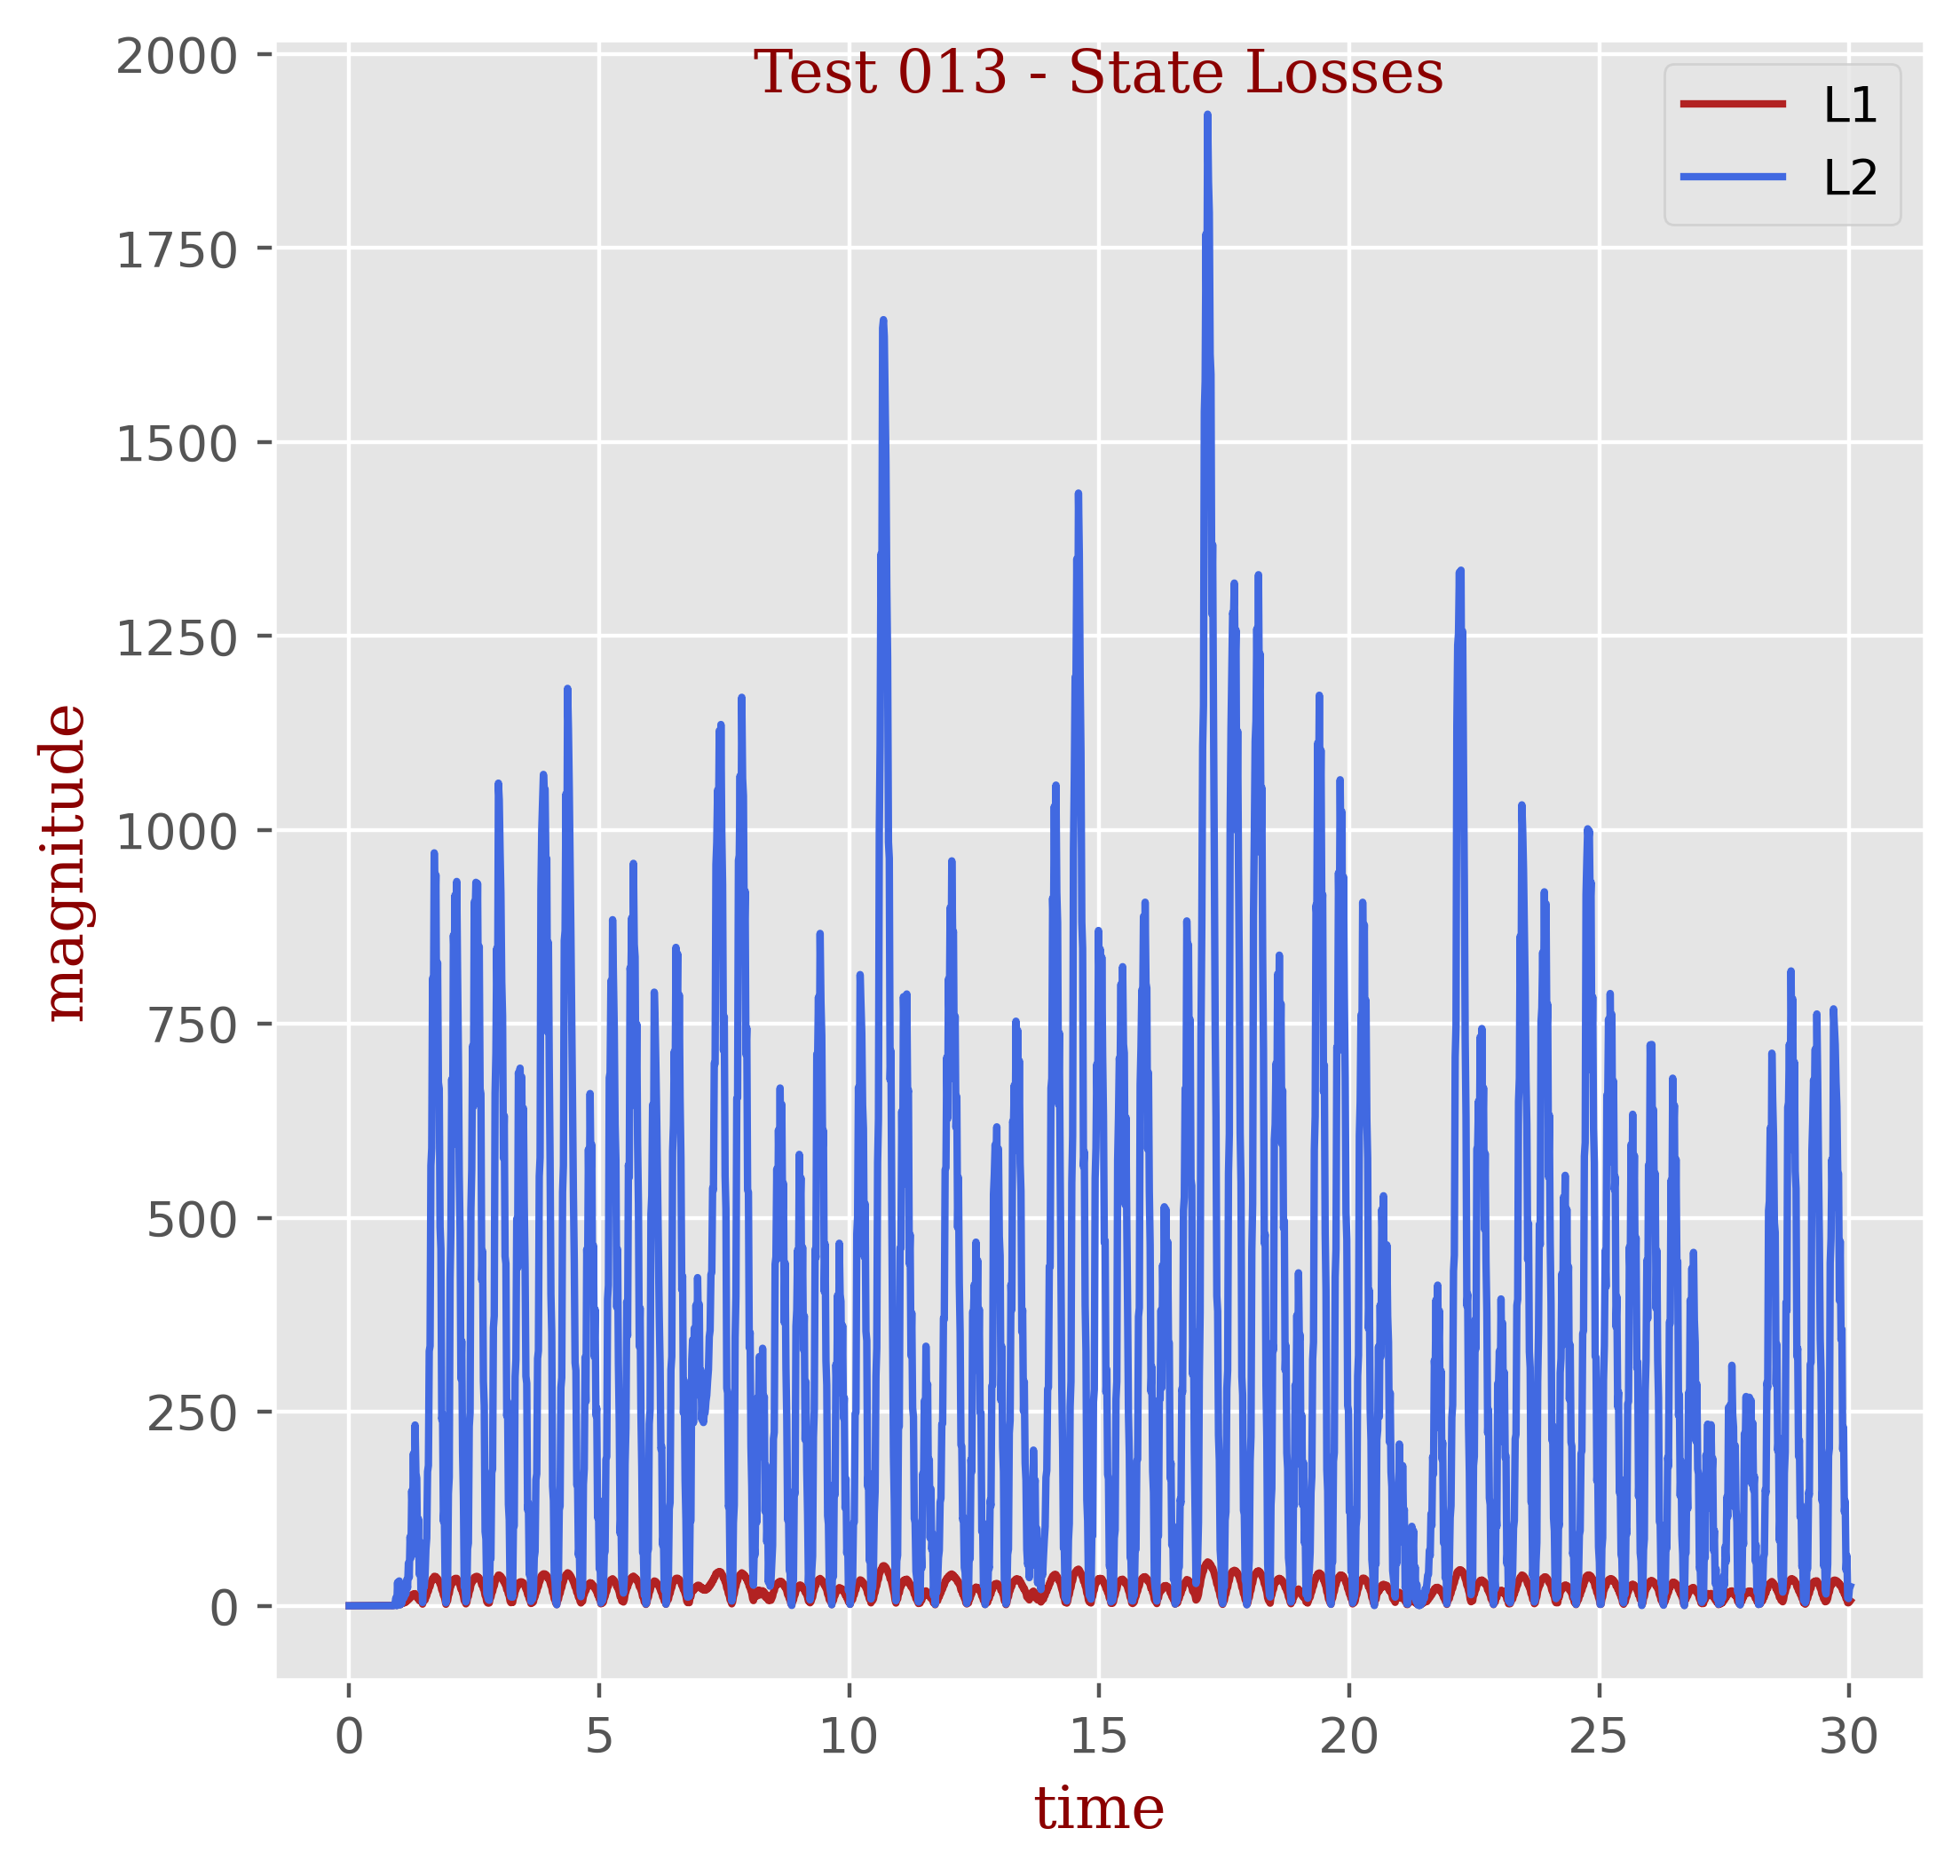
\includegraphics[width=27mm]{Test 013_State_Losses.png}}
\caption{Test 013}
\label{fig:t013}
\end{figure}



\subsection{Experiment II}
In the second experiment, we perform a set of 4 tests with the goal of discoving
some evidence of \emph{chaotic nature} of the system. Although all multi-body
physical systems are chaotic in nature, they vary in degree and it often depends
on system nonlinearities. We wanted to see how fast repeated experiments start
to contradict previous tests with the same configurations and initial conclusions.


\begin{table}[!t]
\renewcommand{\arraystretch}{1.3}
\caption{Experiment II}
\label{tab:002}
\centering
\begin{tabular}{|c||c|c|c|}
\hline
Test ID & duration & sum(L1) & sum(L2) \\
\hline\hline
Test 101 & 20.0  &   6596.9514 & 71827.5496\\
Test 102 & 20.0  &   6596.9514 & 71827.5496\\
Test 103 & \textbf{100.0} &   13095.306 & 77780.4293\\
Test 104 & 100.0 &   \textbf{13096.591} & \textbf{77830.3157}\\
\hline
\end{tabular}
\end{table}


% \newpage



\section{Conclusion}
In this work, we studied the dynamics of a double inverted pendulum on cart
system and examined its nonlinearities with an optimal LQR controller. We
designed this linear controller with complete knowledge of the system and were
only able to achieve UUB stability.
This is indicative of how nonlinear the DIP system is.
Moreover, the high degree system nonlinearity manifests itself in form of
\emph{chaos} and makes the system unrepeatable only after 100 seconds.







% \appendices
% \section{Proof of the First Zonklar Equation}
% Appendix one text goes here.

% you can choose not to have a title for an appendix
% if you want by leaving the argument blank
% \section{Appx B title}
% Appendix two text goes here.


% use section* for acknowledgement
\section*{Acknowledgment}
We want to thank Dr. Frank Lewis for his great lectures, and notes, books, and
materials he made available us (students) throughout the semester.

\bibliography{ref}
\bibliographystyle{ieeetr}

% \begin{thebibliography}{1}

% \bibitem{IEEEhowto:kopka}
% H.~Kopka and P.~W. Daly, \emph{A Guide to \LaTeX}, 3rd~ed.\hskip 1em plus
%   0.5em minus 0.4em\relax Harlow, England: Addison-Wesley, 1999.

% \end{thebibliography}

% biography section
%
% If you have an EPS/PDF photo (graphicx package needed) extra braces are
% needed around the contents of the optional argument to biography to prevent
% the LaTeX parser from getting confused when it sees the complicated
% \includegraphics command within an optional argument. (You could create
% your own custom macro containing the \includegraphics command to make things
% simpler here.)
%\begin{biography}[{\includegraphics[width=1in,height=1.25in,clip,keepaspectratio]{mshell}}]{Michael Shell}
% or if you just want to reserve a space for a photo:

% \begin{IEEEbiography}{Michael Shell}
% Biography text here.
% \end{IEEEbiography}

% % if you will not have a photo at all:
% \begin{IEEEbiographynophoto}{John Doe}
% Biography text here.
% \end{IEEEbiographynophoto}

% insert where needed to balance the two columns on the last page with
% biographies
%\newpage


% You can push biographies down or up by placing
% a \vfill before or after them. The appropriate
% use of \vfill depends on what kind of text is
% on the last page and whether or not the columns
% are being equalized.

%\vfill

% Can be used to pull up biographies so that the bottom of the last one
% is flush with the other column.
%\enlargethispage{-5in}



% that's all folks
\end{document}
